\documentclass[12pt]{article}

%==================== PACKAGES ====================
\usepackage[a4paper,margin=0.8in]{geometry}
\usepackage{amsmath,amssymb,amsthm}
\usepackage{enumitem}
\usepackage{bm}
\usepackage{hyperref}
\usepackage{fancyhdr}
\usepackage{xcolor}
\usepackage{array}
\usepackage{booktabs}
\usepackage{tikz}
\usepackage{pgfplots}
\pgfplotsset{compat=1.17}
\usepackage[most]{tcolorbox}
\tcbuselibrary{theorems,skins,breakable}
\usepackage{graphicx}
\usepackage{multicol}
\usepackage{draftwatermark}

%==================================================
% COURSE METADATA
%==================================================
\newcommand{\CourseCode}{MH1301}
\newcommand{\CourseName}{Discrete Mathematics}
\newcommand{\DocType}{Revision Notes}
\newcommand{\AcademicYear}{Academic Year 2025--2026}

%==================================================
% TCOLORBOX THEOREM STYLES
%==================================================

\newtcbtheorem[number within=section]{definition}{Definition}%
{enhanced,
 breakable=false,
 colback=green!5!white,
 colframe=green!40!black,
 colbacktitle=green!50!black,
 coltitle=white,
 fonttitle=\bfseries,
 title filled,
 boxed title style={
   size=small,
   top=2pt, bottom=2pt,
   left=6pt, right=6pt,
   arc=1pt, outer arc=1pt
 },
 boxrule=0.9pt,
 arc=1pt,
 left=8pt, right=8pt, top=10pt, bottom=8pt,
 before skip=12pt, after skip=12pt
}{def}

\newtcbtheorem[number within=section]{theorem}{Theorem}%
{enhanced,
 breakable=false,
 colback=blue!3!white,
 colframe=blue!40!black,
 colbacktitle=blue!55!black,
 coltitle=white,
 fonttitle=\bfseries,
 title filled,
 boxed title style={
   size=small,
   top=2pt, bottom=2pt,
   left=6pt, right=6pt,
   arc=1pt, outer arc=1pt
 },
 boxrule=0.9pt,
 arc=1pt,
 left=8pt, right=8pt, top=10pt, bottom=8pt,
 before skip=12pt, after skip=12pt
}{thm}

\newtcolorbox{keyformula}[1][]{
    enhanced,
    breakable=false,
    colback=blue!5!white,
    colframe=blue!75!black,
    title=Key Formula,
    fonttitle=\bfseries,
    boxrule=0.9pt,
    arc=2pt,
    left=8pt, right=8pt, top=8pt, bottom=8pt,
    #1
}

\newtcolorbox{examplebox}[1][]{
    enhanced,
    breakable=false,
    colback=brown!5!white,
    colframe=brown!75!black,
    title=Worked Example,
    fonttitle=\bfseries,
    boxrule=0.9pt,
    arc=2pt,
    left=8pt, right=8pt, top=8pt, bottom=8pt,
    #1
}

\newtcolorbox{commonmistake}[1][]{
    enhanced,
    breakable=false,
    colback=red!5!white,
    colframe=red!75!black,
    title=Common Mistake,
    fonttitle=\bfseries,
    boxrule=0.9pt,
    arc=2pt,
    left=8pt, right=8pt, top=8pt, bottom=8pt,
    #1
}

\newtcolorbox{policynote}[1][]{
    enhanced,
    breakable=false,
    colback=yellow!10!white,
    colframe=orange!75!black,
    title=Policy Application,
    fonttitle=\bfseries,
    boxrule=0.9pt,
    arc=2pt,
    left=8pt, right=8pt, top=8pt, bottom=8pt,
    #1
}

\newtcolorbox{examtip}[1][]{
    enhanced,
    breakable=false,
    colback=purple!5!white,
    colframe=purple!75!black,
    title=Exam Focus,
    fonttitle=\bfseries,
    boxrule=0.9pt,
    arc=2pt,
    left=8pt, right=8pt, top=8pt, bottom=8pt,
    #1
}

\newtcolorbox{extension}[1][]{
    enhanced,
    breakable=false,
    colback=cyan!5!white,
    colframe=cyan!75!black,
    title=Extension,
    fonttitle=\bfseries,
    boxrule=0.9pt,
    arc=2pt,
    left=8pt, right=8pt, top=8pt, bottom=8pt,
    #1
}

%==================================================
% TITLE / HEADER / FOOTER / WATERMARK
%==================================================

\title{%
    \vspace{-0.5cm}
    {\Large\bfseries \CourseCode\ \CourseName{} -- \DocType}
}

\author{\AcademicYear \\[0.3em]
\textit{\href{https://qrsntu.org}{\color{black}Quantitative Research Society @ NTU}}}
\date{\today}

\pagestyle{fancy}
\fancyhf{}
\fancyhead[L]{\CourseCode\ \CourseName{} -- \DocType}
\fancyhead[R]{\href{https://qrsntu.org}{QRS@NTU}}
\fancyfoot[C]{\thepage}
\renewcommand{\headrulewidth}{0.4pt}
\renewcommand{\footrulewidth}{0pt}

\SetWatermarkText{QRS@NTU --- qrsntu.org}
\SetWatermarkScale{1}
\SetWatermarkLightness{0.99}

\fancypagestyle{main}{
  \fancyhf{}
  \fancyhead[L]{\CourseCode\ \CourseName{} -- \DocType}
  \fancyhead[R]{\href{https://qrsntu.org}{QRS@NTU}}
  \fancyfoot[C]{\thepage}
  \renewcommand{\headrulewidth}{0.4pt}
  \renewcommand{\footrulewidth}{0pt}
}

\fancypagestyle{plainfirst}{
  \fancyhf{}
  \renewcommand{\headrulewidth}{0pt}
  \renewcommand{\footrulewidth}{0pt}
  \fancyfoot[C]{\scriptsize\textcolor{gray}{\textit{For academic reference only.
 This document is provided for educational purposes and does not constitute an
 official question paper, answer key, or any formally authorised academic
 material. Its content is not guaranteed to be complete or accurate.}}}
}

\hypersetup{
    colorlinks=true,
    linkcolor=blue,
    filecolor=magenta,
    urlcolor=cyan,
    pdftitle={\CourseCode\ \CourseName{} -- \DocType},
    pdfauthor={Quantitative Research Society, NTU},
    pdfsubject={\CourseName},
    pdfkeywords={MH1301, discrete mathematics, counting, recurrence relations, graph theory, QRS@NTU}
}

\setcounter{tocdepth}{3}
\allowdisplaybreaks

%==================================================
% DOCUMENT
%==================================================
\begin{document}
\maketitle
\thispagestyle{plainfirst}

\begin{abstract}
\noindent
These revision notes are organised around the official MH1301 handout sequence for AY2025/2026. The main body is split by part and handout, while the appendix collects compact reference material: notation, core identities, proof patterns, revision checklists, and common pitfalls. Chapter-level mathematical development remains inside dedicated chapter files so that the project can grow cleanly across the whole module.
\end{abstract}

\vspace{0.5cm}

\newpage
\tableofcontents
\newpage

\newgeometry{left=0.72in,right=0.72in,top=0.95in,bottom=0.95in}
\fontsize{10.5pt}{11.9pt}\selectfont
\pagestyle{main}

%==================================================
\section*{How to Use This Document}
\addcontentsline{toc}{section}{How to Use This Document}
%==================================================

\subsection*{1. Purpose of the notes}

These notes are designed to be more than a typed copy of lecture material and less than a full textbook. Their purpose is to give a \emph{revision-oriented working version} of MH1301: each handout is reorganised so that definitions, standard counting mechanisms, proof patterns, and common traps appear in a form that is useful both during the semester and during exam preparation.

The guiding principle is that discrete mathematics is not well revised by memorising isolated answers. Most questions in this module are solved by choosing a correct representation of the objects being counted or analysed. For that reason, the notes repeatedly emphasise the following workflow:
\[
\begin{aligned}
\text{identify the objects}
&\ \longrightarrow\ \text{decide the right model}\\
&\ \longrightarrow\ \text{choose the right counting/proof tool}\\
&\ \longrightarrow\ \text{check edge cases and overlap.}
\end{aligned}
\]

A useful way to think about the document is the following.
\begin{itemize}[leftmargin=*]
    \item The \textbf{main exposition} tells you what the formal statements mean and when they should be used.
    \item The \textbf{worked examples} show how those statements appear in actual MH1301-style questions.
    \item The \textbf{common mistake} boxes tell you where students usually lose marks.
    \item The \textbf{exam focus} boxes isolate high-yield checks, recognition patterns, or revision routines.
    \item The \textbf{extension} boxes provide concise structural viewpoints that are valuable once the core syllabus statement is already understood.
\end{itemize}

Used properly, the notes should help you move from passive recognition (``I have seen this formula before'') to active control (``I can recognise the type of problem, justify the method, and reproduce the argument myself'').

\subsection*{2. Structure by part and handout}

The document follows the module handout structure rather than reorganising the entire course by topic. This is deliberate. In revision, it is useful to preserve the same broad sequencing as lectures while making the internal structure of each handout more explicit.

\begin{itemize}[leftmargin=*]
    \item \textbf{Part I: Counting.} These handouts develop the modelling language of the course: product rule, sum rule, inclusion--exclusion, permutations, combinations, binomial ideas, and related methods. Much of the rest of the module still relies on the same discipline of representing objects carefully.
    \item \textbf{Part II: Recurrence Relations.} These handouts shift from static counting formulas to recursively defined sequences. When revising this part, it is especially important to distinguish the recurrence itself, the initial conditions, and the method used to derive a closed form.
    \item \textbf{Part III: Graph Theory.} These handouts introduce graph language, degree arguments, connectivity, paths, cycles, and trees. Here the emphasis moves from counting choices to verifying definitions and applying structural theorems correctly.
\end{itemize}

Within each chapter file, the intended reading order is usually:
\begin{enumerate}[leftmargin=*]
    \item definitions and basic notation;
    \item main theorems or counting rules;
    \item short examples showing immediate use;
    \item higher-value techniques or interpretations;
    \item end-of-section reminders and pitfalls.
\end{enumerate}

This order matters. If you read examples without first knowing exactly what a theorem says, you tend to remember the surface story of the example rather than the reusable method.

\subsection*{3. How to read the different box types}

These notes use a box system to separate different kinds of information. The boxes are not decorative; they are intended to change how you read.

\begin{center}
\small
\begin{tabular}{@{}p{0.18\textwidth}p{0.72\textwidth}@{}}
\toprule
\textbf{Box type} & \textbf{How to use it} \\
\midrule
Definition & Read slowly enough that you could restate the definition in your own words and also recognise a disguised use of it in a question. \\
Theorem & Learn both the formal statement and the trigger for using it. A theorem is useful only when you can recognise its hypotheses in a new problem. \\
Key Formula & Use as a compact memory anchor only after you understand why the formula is true and what assumptions make it valid. \\
Worked Example & Cover the solution first and try to predict the method. When reading the solution, focus on the decision points rather than the final algebra. \\
Common Mistake & Treat as a pre-commitment check. Before attempting tutorial questions, scan the nearby mistake boxes and actively avoid those errors. \\
Exam Focus & Use as a high-yield checklist. These boxes are especially useful in the week before a test, when you want rapid reminders of recognition patterns and final checks. \\
Extension & Read only after the core argument is secure. Extensions are intended to sharpen understanding, not replace the main route through the material. \\
\bottomrule
\end{tabular}
\end{center}

A common bad habit is to treat boxed material as content to memorise and ordinary paragraphs as content to skip. That is usually backwards. The ordinary paragraphs explain why the box exists, what kind of question it answers, and what limitation it has.

\subsection*{4. Four stages of revision}

\textbf{First learning.}
During the first pass through a handout, the goal is not speed. Read definitions carefully, rewrite the main theorem statements by hand, and pause before each worked example to ask what information in the question tells you which tool is appropriate. At this stage, the notes should be read with the lecture slides or tutorial sheet nearby.

\textbf{Weekly consolidation.}
At the end of each teaching week, revisit the relevant section and reduce it to a shorter personal summary. For counting material, list the standard recognition cues: when a problem is sequential, when cases are disjoint, when overlap forces inclusion--exclusion, when a bijection is more natural than direct counting, and when complement counting is cleaner than direct counting. For recurrence material, summarise which class of recurrence you have seen and which solving mechanism belongs to it. For graph theory, list the definitions and theorem triggers that are easiest to confuse.

\textbf{Pre-midterm review.}
At this stage the notes should no longer be read linearly from page 1 onward. Instead, revise by question type. For example, in the counting part, group together all questions that rely primarily on product rule, all questions that rely on sum rule with disjoint partition, and all questions where overlap detection is the real issue. Use the worked examples as checkpoints, not as reading material. You should be able to reconstruct their structure without copying them line by line.

\textbf{Pre-final review.}
Before the final, the priority is integration. You should be able to move across parts of the course and identify differences in proof style. Counting questions often demand careful modelling; recurrence questions demand algebra plus indexing discipline; graph theory questions demand precise use of definitions and theorem hypotheses. At this stage, the notes are most useful when used diagnostically: identify which theorem statements you can still recognise but not reproduce, which examples you understand only after reading, and which common mistakes you still make under time pressure.

\begin{examtip}[title={A productive revision cycle}]
For any section, a strong short revision cycle is:
\begin{enumerate}[leftmargin=*]
    \item read the definitions and theorem statements once without looking at examples;
    \item close the notes and restate the main ideas from memory;
    \item attempt one tutorial-style question cold;
    \item reopen the notes only to check the exact step where your reasoning diverged.
\end{enumerate}
This is substantially more effective than rereading the same worked solution several times.
\end{examtip}

\subsection*{5. How to read theorem statements productively}

A theorem should not be read as a sentence to be memorised mechanically. For revision purposes, every theorem in MH1301 should be read with four questions in mind:
\begin{enumerate}[leftmargin=*]
    \item \textbf{What are the hypotheses?} What must be true before the theorem can be used?
    \item \textbf{What is the conclusion?} What exactly does the theorem allow me to claim?
    \item \textbf{What class of problem does this theorem solve?} In practice, what does a question look like when this theorem is the right tool?
    \item \textbf{What goes wrong if a hypothesis fails?} Is there a standard overcounting, missing-case, or false-conclusion trap?
\end{enumerate}

For example, the sum rule is not ``add counts whenever you see an \emph{or}.'' It is a statement about \emph{disjoint} unions. Similarly, inclusion--exclusion is not merely a correction formula to memorise; it is the right response when classes overlap in a controlled way. Reading the theorem with its hypotheses foregrounded prevents many routine mistakes.

\subsection*{6. How to use worked examples without becoming passive}

Worked examples are most valuable when they are used actively. A good procedure is:
\begin{enumerate}[leftmargin=*]
    \item Cover the solution.
    \item Read only the question and identify the combinatorial objects involved.
    \item Decide which rule, theorem, or representation is most likely to be relevant.
    \item Write the first two or three lines yourself.
    \item Only then compare with the notes.
\end{enumerate}

When comparing with the written solution, do not ask only whether the final answer matches. Ask instead:
\begin{itemize}[leftmargin=*]
    \item Did I partition the cases in the same way?
    \item Did I justify why the chosen rule applies?
    \item Did I ignore an overlap or edge case?
    \item Could I produce the same argument again tomorrow without seeing it?
\end{itemize}

If an example feels easy only when the solution is visible, then it is not yet learned.

\subsection*{7. How to use special techniques and extensions properly}

Special techniques and extension boxes are included because exam-level understanding often requires more than the shortest syllabus statement. However, they should be used in the right order. The core path is always:
\[
\text{definition} \longrightarrow \text{main theorem/rule} \longrightarrow \text{standard example}.
\]
Only after that should you use the extensions to deepen or compress your thinking.

Typical uses of extension material include:
\begin{itemize}[leftmargin=*]
    \item seeing why a bijection is canonical rather than ad hoc;
    \item understanding inclusion--exclusion through indicator-style reasoning;
    \item recognising a more elegant derivation after mastering the standard derivation;
    \item seeing how one theorem packages several simpler observations into one structural statement.
\end{itemize}

Used properly, extensions improve retention because they connect ideas. Used too early, they can make the notes look more advanced than they are. The right test is simple: if you cannot yet do the core example unassisted, return to the main exposition first.

\subsection*{8. Do not treat the notes as a formula sheet}

These notes contain formulas and compact summaries, but MH1301 is not a formula-substitution module. Many wrong answers in discrete mathematics arise not because a formula is forgotten, but because the student counts the wrong set, assumes cases are disjoint when they are not, forgets that order matters, or applies a theorem outside its valid setting.

For that reason, every time you use a formula, you should still ask:
\begin{itemize}[leftmargin=*]
    \item What set is being counted?
    \item Why does this object decompose into stages or cases in the way I claim?
    \item Is the representation ordered or unordered?
    \item Is repetition allowed?
    \item Are the cases disjoint, or must I correct overlap?
\end{itemize}

The formula then becomes the final compression of a correct model, not a substitute for one.

\subsection*{9. How to cross-check understanding}

A reliable test of understanding is whether you can reproduce an argument without immediately looking back at the notes. Useful self-checks include:
\begin{itemize}[leftmargin=*]
    \item restating a theorem from memory and identifying its hypotheses;
    \item reconstructing the proof idea of a short result, even if not every word matches the written version;
    \item solving a nearby tutorial question using the same core method but with different numbers or conditions;
    \item explaining aloud why a tempting incorrect method fails.
\end{itemize}

In practical use, the notes should be paired with tutorial questions, short self-quizzes, and timed practice. After reading a section, attempt at least one question for which you do \emph{not} already know the answer. The objective is not to finish the notes; it is to become able to produce the reasoning independently.

\begin{extension}[title={Using these notes at high intensity near an exam}]
When time is short, do not reread whole chapters uniformly. Instead, scan the theorem statements and exam-focus boxes, then choose only the sections where you cannot immediately answer the question: \emph{Could I reconstruct the main argument here on a blank page?} This triages revision toward genuine weaknesses rather than familiar pages.
\end{extension}

\newpage

%==================================================
\section*{Course Roadmap}
\addcontentsline{toc}{section}{Course Roadmap}
%==================================================

\subsection*{Part I: Counting}
\begin{itemize}[leftmargin=*]
    \item Handout 01 --- Basics of Counting
    \item Handout 02 --- Pigeonhole Principle, Permutations and Combination
    \item Handout 03 --- Binomial Theorem, Generalized Permutations and Combination
\end{itemize}

\subsection*{Part II: Recurrence Relations}
\begin{itemize}[leftmargin=*]
    \item Handout 04 --- Recurrence Relations
    \item Handout 05 --- Linear Homogeneous Recurrence Relations
    \item Handout 06 --- Linear Non-Homogeneous Recurrence Relations
\end{itemize}

\subsection*{Part III: Graph Theory}
\begin{itemize}[leftmargin=*]
    \item Handout 07 --- Graph Theory (1)
    \item Handout 08 --- Graph Theory (2)
    \item Handout 09 --- Graph Theory (3)
    \item Handout 10 --- Graph Theory (4)
    \item Handout 11 --- Graph Theory (5)
    \item Handout 12 --- Trees
\end{itemize}

\begin{examtip}[title={What changes across the three parts}]
In Part I, most questions are solved by modelling and counting. In Part II, the main challenge is setting up and solving recurrences with the correct indexing and initial conditions. In Part III, precision of definitions becomes even more important: many graph questions are easy to state informally but require exact theorem use to solve cleanly.
\end{examtip}

\newpage

%==================================================
% CHAPTERS
%==================================================

\IfFileExists{chapters/handout01.tex}{\part{Counting}
\section{Handout 01: Basics of Counting}

\subsection{Overview}

This handout introduces the basic counting language used throughout MH1301. The central lesson is not merely that one should know several formulas, but that one should first identify the \emph{right mathematical model} for the objects in the question. A counting problem becomes manageable only after it is written as a problem about sets, sequences, functions, binary strings, disjoint cases, or overlapping cases.

The core topics of this handout are:
\begin{itemize}[leftmargin=*]
    \item reminders on sets and cardinality;
    \item the distinction between sequences and sets;
    \item the product rule and permutations;
    \item counting functions between finite sets;
    \item injective, surjective, and bijective functions;
    \item counting by bijection;
    \item binary strings and subsets;
    \item the sum rule;
    \item inclusion--exclusion for two sets, three sets, and the general case.
\end{itemize}

\begin{examtip}[title={The guiding question of Handout 01}]
Before counting, ask: \emph{What is a single object here?} If you identify the object incorrectly, the rest of the calculation is usually wrong even if the arithmetic is flawless.
\end{examtip}

%==================================================
\subsection{Sets, Cardinality, and Counting}
%==================================================

\begin{definition}{Set and cardinality}{set-cardinality}
A \emph{set} is an unordered collection of objects, called its elements. If $S$ is finite, its \emph{cardinality} $|S|$ is the number of distinct elements in $S$.
\end{definition}

The set viewpoint matters because counting is fundamentally the task of determining the size of an explicitly defined set. Two reminders from elementary set theory are especially important in this chapter:
\begin{itemize}[leftmargin=*]
    \item the order in which elements are listed in a set is irrelevant;
    \item repeated listing does not create new elements.
\end{itemize}

Thus
\[
\{a,b,c\}=\{b,c,a\}=\{a,b,c,a\}
\qquad\text{and hence}\qquad
|\{a,b,c,a\}|=3.
\]

\begin{definition}{Subset}{subset}
If $A$ and $B$ are sets, then $A\subseteq B$ means that every element of $A$ is also an element of $B$.
\end{definition}

\begin{examplebox}[title={Why the notion of a set matters in counting}]
If a problem asks for the number of subsets of $\{1,2,3\}$, the objects being counted are
\[
\varnothing,\ \{1\},\ \{2\},\ \{3\},\ \{1,2\},\ \{1,3\},\ \{2,3\},\ \{1,2,3\}.
\]
The expressions $\{1,2\}$ and $\{2,1\}$ represent the same subset, so they should not be counted separately.
\end{examplebox}

\begin{commonmistake}[title={Counting symbols instead of distinct elements}]
The notation used to display a set is not the object itself. Repeated entries and reordered entries do not change the set. This is one of the earliest places where overcounting can happen.
\end{commonmistake}

%==================================================
\subsection{Sequences versus Sets}
%==================================================

\begin{definition}{Sequence}{sequence}
A \emph{sequence} is an ordered collection of elements, not necessarily distinct.
\end{definition}

This contrasts sharply with the notion of a set. In a sequence, position matters; in a set, it does not.

\begin{examplebox}[title={Basic contrast}]
The sequences
\[
(a,b,c),\qquad (b,a,c),\qquad (a,b,a)
\]
are generally different. By contrast,
\[
\{a,b,c\}=\{b,a,c\}
\]
as sets.
\end{examplebox}

\begin{examtip}[title={Recognition pattern}]
Words such as \emph{string}, \emph{code}, \emph{password}, \emph{arrangement}, \emph{line up}, and \emph{permutation} usually indicate that the relevant object is a sequence rather than a set.
\end{examtip}

%==================================================
\subsection{Product Rule}
%==================================================

\begin{theorem}{Product Rule}{product-rule}
Suppose a set $S$ consists of sequences of length $k$, where there are $n_1$ possible first entries, $n_2$ possible second entries for each first entry, and so on up to $n_k$ possible $k$-th entries for each compatible previous choice. Then
\[
|S|=n_1n_2\cdots n_k.
\]
\end{theorem}

The product rule is the rule for \emph{sequential construction}. It applies when an object can be built in stages and each stage has a known number of possibilities.

\begin{examplebox}[title={Die and coin}]
When a six-sided die and a two-sided coin are tossed together, an outcome is an ordered pair
\[
(\text{die outcome},\text{coin outcome}).
\]
There are $6$ choices for the first component and $2$ for the second, so the total number of outcomes is
\[
6\cdot 2=12.
\]
\end{examplebox}

\begin{examplebox}[title={License plates}]
If each plate consists of a sequence of $3$ letters followed by $3$ digits, then the number of possible plates is
\[
26^3\cdot 10^3=17{,}576{,}000.
\]
This is a direct product-rule problem because each position is filled in sequence.
\end{examplebox}

\begin{examplebox}[title={Tutorial 1, Question 1(a)}]
How many different three-letter initials are possible if there are $26$ letters?

\textbf{Solution.}
Each of the three positions may be filled by any of $26$ letters, so the total number is
\[
26^3=17{,}576.
\]
\end{examplebox}

\begin{extension}[title={Decision-tree viewpoint for the product rule}]
One can visualise the product rule using a decision tree: each level corresponds to one stage of the choice process, and each root-to-leaf path corresponds to one completed object. If every path has $n_1,n_2,\dots,n_k$ choices at the respective levels, then the total number of leaves is $n_1n_2\cdots n_k$.
\end{extension}

\begin{commonmistake}[title={Multiplying visible numbers without identifying stages}]
The product rule applies because an object is built step by step, not because several numbers happen to appear in the question. If the stages are not well defined, multiplication may be unjustified.
\end{commonmistake}

%==================================================
\subsection{Permutations}
%==================================================

\begin{definition}{Permutation}{permutation}
A \emph{permutation} of a finite set $S$ is a sequence containing every element of $S$ exactly once.
\end{definition}

\begin{theorem}{Number of permutations}{permutation-count}
If $|S|=n$, then the number of permutations of $S$ is
\[
n!.
\]
\end{theorem}

\begin{proof}
For the first position, there are $n$ choices. After choosing one element, there are $n-1$ choices for the second position, then $n-2$ for the third, and so on, until one choice remains for the last position. By the product rule,
\[
n(n-1)(n-2)\cdots 2\cdot 1=n!.
\]
\end{proof}

\begin{examplebox}[title={Permutations of $\{1,2,3\}$}]
The permutations are
\[
(1,2,3),\ (1,3,2),\ (2,1,3),\ (2,3,1),\ (3,1,2),\ (3,2,1),
\]
so there are $3!=6$ of them.
\end{examplebox}

\begin{examtip}[title={Recognition pattern for permutations}]
If a problem asks for orderings of distinct objects without repetition, factorial growth is usually present. Still, one should justify which objects occupy which positions rather than writing $n!$ immediately.
\end{examtip}

%==================================================
\subsection{Functions and Counting Functions}
%==================================================

\begin{definition}{Function}{function}
Let $X$ and $Y$ be sets. A function $f:X\to Y$ assigns to each element $x\in X$ exactly one element $f(x)\in Y$.
\end{definition}

\begin{examplebox}[title={What is and is not a function}]
The rule $f(x)=x^2$ is a function because each input has exactly one output. By contrast, the rule $f(x)=\pm\sqrt{x}$ is not a function from the nonnegative reals to the reals, because one input generally has two possible outputs.
\end{examplebox}

\begin{theorem}{Counting all functions}{count-functions}
If $|X|=m$ and $|Y|=n$, then the number of functions from $X$ to $Y$ is
\[
n^m.
\]
\end{theorem}

\begin{proof}
Each element of the domain $X$ independently chooses one image in $Y$. Since there are $m$ domain elements and $n$ choices for each, the product rule gives
\[
\underbrace{n\cdot n\cdots n}_{m\text{ times}}=n^m.
\]
\end{proof}

\begin{examplebox}[title={A function-counting model}]
If $|X|=4$ and $|Y|=3$, then each of the $4$ elements of $X$ chooses one of $3$ images in $Y$, so the number of functions $X\to Y$ is
\[
3^4=81.
\]
\end{examplebox}

\begin{commonmistake}[title={Why the answer is $n^m$, not $mn$}]
The quantity $mn$ would count ordered pairs $(x,y)$ with $x\in X$ and $y\in Y$, not functions from $X$ to $Y$. A function requires an image choice for \emph{every} element of the domain.
\end{commonmistake}

%==================================================
\subsection{Injective, Surjective, and Bijective Functions}
%==================================================

\begin{definition}{Injective, surjective, bijective}{inj-surj-bij}
Let $f:X\to Y$.
\begin{itemize}[leftmargin=*]
    \item $f$ is \emph{injective} if distinct elements of $X$ have distinct images.
    \item $f$ is \emph{surjective} if every element of $Y$ is the image of at least one element of $X$.
    \item $f$ is \emph{bijective} if it is both injective and surjective.
\end{itemize}
\end{definition}

% Fallback description: three simple mapping diagrams illustrating surjective/non-injective, injective/non-surjective, and bijective maps.
\begin{center}
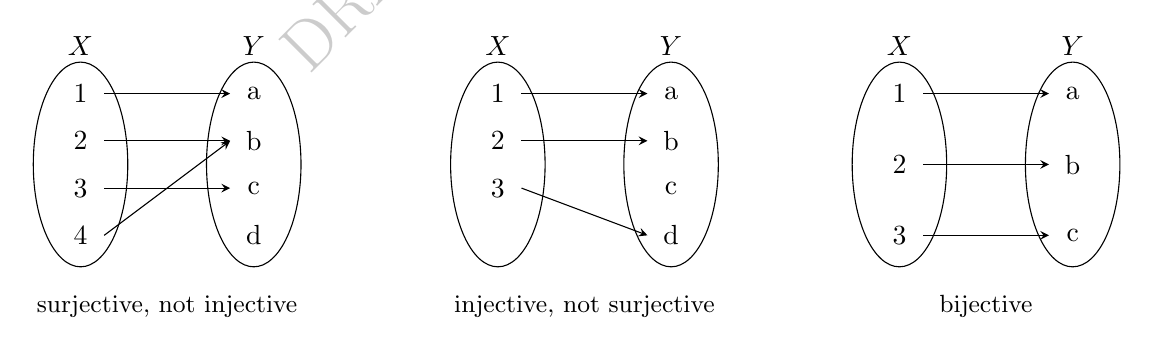
\begin{tikzpicture}[x=1cm,y=1cm,>=stealth]
    \draw (0,0) ellipse (0.6 and 1.3);
    \draw (2.2,0) ellipse (0.6 and 1.3);
    \node at (0,1.5) {$X$};
    \node at (2.2,1.5) {$Y$};
    \foreach \y/\lab in {0.9/1,0.3/2,-0.3/3,-0.9/4}
        \node at (0,\y) {\lab};
    \foreach \y/\lab in {0.9/a,0.3/b,-0.3/c,-0.9/d}
        \node at (2.2,\y) {\lab};
    \draw[->] (0.3,0.9) -- (1.9,0.9);
    \draw[->] (0.3,0.3) -- (1.9,0.3);
    \draw[->] (0.3,-0.3) -- (1.9,-0.3);
    \draw[->] (0.3,-0.9) -- (1.9,0.3);
    \node at (1.1,-1.8) {\small surjective, not injective};

    \begin{scope}[shift={(5.3,0)}]
        \draw (0,0) ellipse (0.6 and 1.3);
        \draw (2.2,0) ellipse (0.6 and 1.3);
        \node at (0,1.5) {$X$};
        \node at (2.2,1.5) {$Y$};
        \foreach \y/\lab in {0.9/1,0.3/2,-0.3/3}
            \node at (0,\y) {\lab};
        \foreach \y/\lab in {0.9/a,0.3/b,-0.3/c,-0.9/d}
            \node at (2.2,\y) {\lab};
        \draw[->] (0.3,0.9) -- (1.9,0.9);
        \draw[->] (0.3,0.3) -- (1.9,0.3);
        \draw[->] (0.3,-0.3) -- (1.9,-0.9);
        \node at (1.1,-1.8) {\small injective, not surjective};
    \end{scope}

    \begin{scope}[shift={(10.4,0)}]
        \draw (0,0) ellipse (0.6 and 1.3);
        \draw (2.2,0) ellipse (0.6 and 1.3);
        \node at (0,1.5) {$X$};
        \node at (2.2,1.5) {$Y$};
        \foreach \y/\lab in {0.9/1,0.0/2,-0.9/3}
            \node at (0,\y) {\lab};
        \foreach \y/\lab in {0.9/a,0.0/b,-0.9/c}
            \node at (2.2,\y) {\lab};
        \draw[->] (0.3,0.9) -- (1.9,0.9);
        \draw[->] (0.3,0.0) -- (1.9,0.0);
        \draw[->] (0.3,-0.9) -- (1.9,-0.9);
        \node at (1.1,-1.8) {\small bijective};
    \end{scope}
\end{tikzpicture}
\end{center}

\begin{theorem}{Cardinality constraints for finite sets}{map-cardinality}
Let $X$ and $Y$ be finite sets and let $f:X\to Y$.
\begin{itemize}[leftmargin=*]
    \item If $f$ is injective, then $|X|\le |Y|$.
    \item If $f$ is surjective, then $|X|\ge |Y|$.
    \item If $f$ is bijective, then $|X|=|Y|$.
\end{itemize}
\end{theorem}

These facts are often called mapping rules. They are especially useful because they allow set sizes to be compared without counting both sets directly.

\begin{extension}[title={Bijections are exact counting transfers}]
A bijection does more than show two sets have the same size abstractly. It gives a one-to-one translation between their elements. In counting problems this matters because it guarantees that no object is lost and no object is counted twice.
\end{extension}

%==================================================
\subsection{Counting via Bijection}
%==================================================

\begin{definition}{Counting by bijection}{counting-bijection}
To count a difficult finite set $A$, one may construct a bijection from $A$ to a simpler finite set $B$. Since bijections preserve cardinality,
\[
|A|=|B|.
\]
\end{definition}

This is one of the most powerful ideas in discrete mathematics. Often the original objects are awkward, but a good encoding turns them into strings, subsets, or functions that can be counted immediately.

\begin{examtip}[title={Bijection checklist}]
When using a bijection, verify three things explicitly:
\begin{enumerate}[leftmargin=*]
    \item the encoding is well defined;
    \item different original objects cannot map to the same code;
    \item every valid code comes from an original object.
\end{enumerate}
\end{examtip}

%==================================================
\subsection{Binary Strings and Subsets}
%==================================================

\begin{definition}{Binary string}{binary-string}
An \emph{$n$-bit binary string} is a sequence $(b_1,\dots,b_n)$ in which each $b_i\in\{0,1\}$.
\end{definition}

\begin{theorem}{Counting binary strings}{count-binary}
The number of binary strings of length $n$ is
\[
2^n.
\]
\end{theorem}

\begin{proof}
Each of the $n$ positions has two possible entries, $0$ or $1$. By the product rule, the total number of strings is $2^n$.
\end{proof}

\begin{examplebox}[title={Tutorial 1, Question 2(b)}]
How many bit strings of length $n$ start and end with $1$?

\textbf{Solution.}
If $n=1$, there is exactly one such string, namely $1$.
For $n\ge 2$, the first and last positions are fixed, and the remaining $n-2$ positions are arbitrary. Hence the number is
\[
2^{n-2}\qquad (n\ge 2).
\]
\end{examplebox}

\begin{theorem}{Number of subsets of a finite set}{power-set-count}
If $S=\{1,2,\dots,n\}$, then the number of subsets of $S$ is
\[
2^n.
\]
\end{theorem}

\begin{proof}
Associate to each subset $A\subseteq S$ the binary string $(b_1,\dots,b_n)$ defined by
\[
b_i=
\begin{cases}
1,& i\in A,\\
0,& i\notin A.
\end{cases}
\]
This is a bijection between subsets of $S$ and binary strings of length $n$. Since there are $2^n$ such strings, there are $2^n$ subsets of $S$.
\end{proof}

% Fallback description: subset-to-binary-string encoding showing membership positions.
\begin{center}
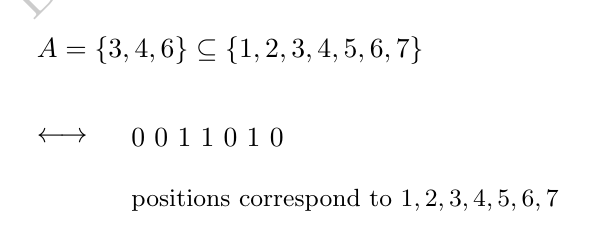
\begin{tikzpicture}[x=1cm,y=1cm]
    \node[anchor=west] at (0,1.1) {$A=\{3,4,6\}\subseteq \{1,2,3,4,5,6,7\}$};
    \node[anchor=west] at (0,0) {$\longleftrightarrow$};
    \node[anchor=west] at (1.2,0) {$0\ 0\ 1\ 1\ 0\ 1\ 0$};
    \node[anchor=west] at (1.2,-0.8) {\small positions correspond to $1,2,3,4,5,6,7$};
\end{tikzpicture}
\end{center}

\begin{examplebox}[title={The standard subset encoding}]
For $S=\{1,2,3,4,5,6,7\}$, the subset $\{3,4,6\}$ corresponds to the string
\[
(0,0,1,1,0,1,0),
\]
because positions $3$, $4$, and $6$ are marked by $1$.
\end{examplebox}

\begin{extension}[title={Characteristic-function viewpoint}]
The binary-string encoding of a subset $A\subseteq S$ can also be viewed as its characteristic function
\[
\chi_A:S\to\{0,1\},
\qquad
\chi_A(s)=
\begin{cases}
1,& s\in A,\\
0,& s\notin A.
\end{cases}
\]
So subset counting is also a function-counting problem: each element of $S$ independently chooses one of two possible outputs.
\end{extension}

%==================================================
\subsection{Sum Rule}
%==================================================

\begin{theorem}{Sum Rule}{sum-rule}
If $A_1,\dots,A_k$ are pairwise disjoint finite sets, then
\[
|A_1\cup\cdots\cup A_k|=|A_1|+\cdots+|A_k|.
\]
\end{theorem}

The sum rule applies when the total collection has been partitioned into disjoint cases. Each object belongs to exactly one case, so simple addition is valid.

\begin{examplebox}[title={Textbooks}]
If there are $26$ MH1301 textbooks in one library and $15$ in another, and the two collections are taken as disjoint holdings, then the total number is
\[
26+15=41.
\]
\end{examplebox}

\begin{examplebox}[title={Passwords of lengths 6, 7, or 8}]
Suppose a password consists of uppercase letters or digits and has length $6$, $7$, or $8$. There are $26+10=36$ choices for each character. Let $X_6$, $X_7$, and $X_8$ denote the sets of passwords of lengths $6$, $7$, and $8$. These sets are disjoint, so
\[
|X_6\cup X_7\cup X_8|=|X_6|+|X_7|+|X_8|=36^6+36^7+36^8.
\]
\end{examplebox}

\begin{extension}[title={Why naive sum rule fails with overlap}]
The equation $|A\cup B|=|A|+|B|$ is not a general union formula; it is a \emph{disjoint-union} formula. The moment one object can satisfy both case descriptions, addition alone overcounts that object.
\end{extension}

\begin{commonmistake}[title={Using ``or'' as a signal for addition}]
The word \emph{or} does not by itself justify the sum rule. One must still check whether the cases are disjoint. If they overlap, the correct tool is inclusion--exclusion or a finer disjoint partition.
\end{commonmistake}

%==================================================
\subsection{Inclusion--Exclusion for Two Sets}
%==================================================

\begin{theorem}{Two-set inclusion--exclusion}{ie-two}
For any finite sets $A$ and $B$,
\[
|A\cup B|=|A|+|B|-|A\cap B|.
\]
\end{theorem}

\begin{proof}
In the sum $|A|+|B|$, elements of $A\setminus B$ and $B\setminus A$ are counted once, while elements of $A\cap B$ are counted twice. Subtracting $|A\cap B|$ corrects the double counting.
\end{proof}

% Fallback description: two-set Venn diagram indicating that the overlap is the region counted twice before correction.
\begin{center}
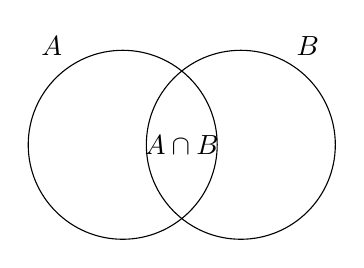
\begin{tikzpicture}[scale=1]
    \draw (0,0) circle (1.2);
    \draw (1.5,0) circle (1.2);
    \node at (-0.9,1.25) {$A$};
    \node at (2.35,1.25) {$B$};
    \node at (0.75,0) {$A\cap B$};
\end{tikzpicture}
\end{center}

\begin{examplebox}[title={Bit strings of length 8}]
How many $0$-$1$ strings of length $8$ either start with $1$ or end with $00$?

\textbf{Solution.}
Let
\[
A=\{\text{strings starting with }1\},
\qquad
B=\{\text{strings ending with }00\}.
\]
Then
\[
|A|=2^7=128,
\qquad
|B|=2^6=64.
\]
Also,
\[
|A\cap B|=2^5=32,
\]
because such a string has the form
\[
1\ \square\ \square\ \square\ \square\ \square\ 0\ 0.
\]
Hence
\[
|A\cup B|=128+64-32=160.
\]
\end{examplebox}

\begin{examplebox}[title={Students taking Mathematics or Physics}]
Suppose there are $1807$ students in total, with $453$ taking Mathematics, $567$ taking Physics, and $299$ taking both. Then the number taking at least one of the two subjects is
\[
453+567-299=721.
\]
Therefore the number taking neither is
\[
1807-721=1086.
\]
\end{examplebox}

\begin{extension}[title={Indicator-style intuition for the two-set formula}]
For each object $x$, the indicator of membership in $A\cup B$ satisfies
\[
1_{A\cup B}(x)=1_A(x)+1_B(x)-1_{A\cap B}(x).
\]
Summing this identity over all objects in the universe gives the cardinality formula. This viewpoint explains inclusion--exclusion as a pointwise correction mechanism rather than a formula to memorise blindly.
\end{extension}

%==================================================
\subsection{Inclusion--Exclusion for Three Sets}
%==================================================

\begin{theorem}{Three-set inclusion--exclusion}{ie-three}
For finite sets $A$, $B$, and $C$,
\[
|A\cup B\cup C|
=
|A|+|B|+|C|
-|A\cap B|-|A\cap C|-|B\cap C|
+|A\cap B\cap C|.
\]
\end{theorem}

\begin{proof}
The first three terms count every element once for each set containing it. Thus an element in exactly two sets is counted twice and must be corrected by subtracting the relevant pairwise intersection. But an element in all three sets is then subtracted three times after being added three times, so it must be added back once.
\end{proof}

% Fallback description: three-set Venn diagram highlighting the central triple-overlap region that is added back at the last step.
\begin{center}
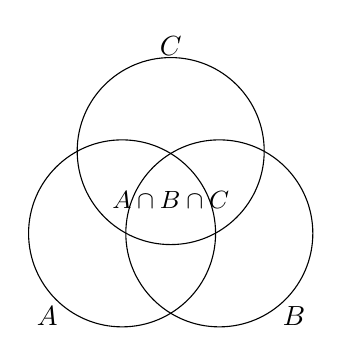
\begin{tikzpicture}[scale=0.95]
    \draw (0,0) circle (1.25);
    \draw (1.3,0) circle (1.25);
    \draw (0.65,1.1) circle (1.25);
    \node at (-1.0,-1.1) {$A$};
    \node at (2.3,-1.1) {$B$};
    \node at (0.65,2.5) {$C$};
    \node at (0.65,0.45) {\small $A\cap B\cap C$};
\end{tikzpicture}
\end{center}

\begin{examplebox}[title={Spanish, French, and Russian courses}]
Suppose
\[
|S|=1232,\quad |F|=879,\quad |R|=114,
\]
\[
|S\cap F|=103,\quad |S\cap R|=23,\quad |F\cap R|=14,
\]
and
\[
|S\cup F\cup R|=2092.
\]
Then
\[
2092=1232+879+114-103-23-14+|S\cap F\cap R|,
\]
so
\[
|S\cap F\cap R|=7.
\]
\end{examplebox}

\begin{extension}[title={Why the signs alternate}]
Inclusion--exclusion alternates signs because each stage corrects the overcorrection from the previous stage. First the single-set counts overcount overlaps, then pairwise subtraction overcorrects the deepest overlaps, then triple intersections restore the correct count, and so on.
\end{extension}

%==================================================
\subsection{General Inclusion--Exclusion Principle}
%==================================================

\begin{theorem}{General inclusion--exclusion principle}{ie-general}
For finite sets $A_1,\dots,A_n$,
\[
\left|\bigcup_{i=1}^n A_i\right|
=
\sum_{i=1}^n |A_i|
-
\sum_{1\le i<j\le n}|A_i\cap A_j|
+
\sum_{1\le i<j<k\le n}|A_i\cap A_j\cap A_k|
-\cdots+
(-1)^{n-1}|A_1\cap\cdots\cap A_n|.
\]
\end{theorem}

A useful verbal memory pattern is:
\begin{center}
add the single-set sizes, subtract the two-way intersections, add the three-way intersections, subtract the four-way intersections, and continue alternating.
\end{center}

\begin{proof}[Sketch of proof]
The standard proof is by induction on $n$.
For $n=1$ and $n=2$, the statement is immediate.
Assume the formula holds for $n$ sets. Then
\[
\bigcup_{i=1}^{n+1}A_i
=
\left(\bigcup_{i=1}^n A_i\right)\cup A_{n+1}.
\]
Applying the two-set inclusion--exclusion formula gives
\[
\left|\bigcup_{i=1}^{n+1}A_i\right|
=
\left|\bigcup_{i=1}^{n}A_i\right|+|A_{n+1}|-
\left|\left(\bigcup_{i=1}^{n}A_i\right)\cap A_{n+1}\right|.
\]
Now use the identity
\[
\left(\bigcup_{i=1}^{n}A_i\right)\cap A_{n+1}
=
\bigcup_{i=1}^{n}(A_i\cap A_{n+1}),
\]
and apply the inductive hypothesis to the two unions. The alternating-sign pattern is preserved, giving the formula for $n+1$ sets.
\end{proof}

\begin{extension}[title={Canonical correction viewpoint}]
General inclusion--exclusion can be understood as a correction algorithm: count everything that qualifies at least once, then remove overcounts, then repair the over-repair, and continue until every object that belongs to the union has net weight exactly $1$.
\end{extension}

%==================================================
\subsection{Special Techniques and Elegant Problem-Solving Ideas}
%==================================================

\subsubsection*{Counting by bijection}
A difficult family of objects is often easier to count after a clean encoding into binary strings, subsets, or functions. The value of a bijection is that it turns a conceptual observation into an exact counting statement.

\subsubsection*{Binary encoding of subsets}
Whenever each labelled element may either be chosen or not chosen, a binary model is natural. This is the fastest route to the formula $2^n$ for subsets of an $n$-element set.

\subsubsection*{Complement counting}
If the desired class is hard to count directly but the excluded class is simple, count the universe and subtract the complement. This frequently appears in string-counting questions involving conditions such as ``at least one'' or ``not all''.

\subsubsection*{Partition before using the sum rule}
If the cases initially overlap, refine them into genuinely disjoint subcases before adding. This is often a cleaner alternative to applying inclusion--exclusion immediately.

\subsubsection*{Detect overlap before counting}
Before adding case counts, always ask whether one object can satisfy two of the case descriptions simultaneously. If yes, direct addition is unsafe.

\subsubsection*{Convert objects into strings or functions}
Many combinatorial objects are best thought of as a finite sequence of labelled decisions. Once the positions and choices are identified, the product rule often becomes immediate.

\begin{examtip}[title={A practical hierarchy of methods for Handout 01}]
For a new counting problem, a good order of attack is:
\begin{enumerate}[leftmargin=*]
    \item try to model the object directly as a sequence of choices;
    \item if cases split naturally, test whether they are disjoint;
    \item if overlap appears, use inclusion--exclusion or refine the partition;
    \item if the objects remain awkward, search for a bijection to a cleaner family.
\end{enumerate}
\end{examtip}

%==================================================
\subsection{Final Consolidation}
%==================================================

\begin{center}
\small
\begin{tabular}{@{}p{0.25\textwidth}p{0.28\textwidth}p{0.37\textwidth}@{}}
\toprule
\textbf{Situation} & \textbf{Primary tool} & \textbf{Typical signal words} \\
\midrule
Sequential choices & Product rule & choose, then, fill positions, assign \\
Ordered arrangement without repetition & Permutations & arrange, order, line up, rank \\
Functions from one finite set to another & Function counting & map each element, assign outputs \\
Equivalent easier model & Bijection & encode, represent, correspond \\
Yes/no choice per label & Binary strings & subset, selected/not selected \\
Disjoint cases & Sum rule & either this case or that case, by length, by type \\
Overlapping cases & Inclusion--exclusion & overlap, at least one, counted twice \\
\bottomrule
\end{tabular}
\end{center}

\begin{commonmistake}[title={Final checklist for Handout 01}]
Before accepting a counting solution, verify:
\begin{enumerate}[leftmargin=*]
    \item Have I identified the objects correctly as sets, sequences, or functions?
    \item Have I justified why the chosen rule applies?
    \item If I used the sum rule, are the cases disjoint?
    \item If I used inclusion--exclusion, did I count the overlap correctly?
    \item If I used a bijection, did I explain why it is one-to-one and onto?
\end{enumerate}
\end{commonmistake}

\begin{examtip}[title={What should remain after this handout}]
After Handout 01, the main skills to retain are: modelling a counting problem as a set problem, recognising when order matters, using the product rule and sum rule correctly, correcting overlap by inclusion--exclusion, and translating objects into easier forms through bijections and binary encodings.
\end{examtip}}{}
\IfFileExists{chapters/handout02.tex}{\part{Counting}
\section{Handout 02: Pigeonhole Principle, Permutations and Combinations}

\subsection{Overview}

This handout continues Part~I on counting. The main themes are:
\begin{itemize}[leftmargin=*]
    \item the pigeonhole principle and its generalized form;
    \item permutations and $r$-permutations as \emph{ordered} selections;
    \item combinations as \emph{unordered} selections;
    \item the relation
    \[
    P(n,r)=\binom{n}{r}r!;
    \]
    \item combinatorial proof, where one proves an identity by counting the same set in two different ways.
\end{itemize}

The central revision goal is to distinguish carefully between three recurring operations:
\[
\text{force existence},\qquad \text{choose and order},\qquad \text{choose without order}.
\]

\begin{examtip}[title={Main recognition goals for this handout}]
A typical question in this handout usually asks for one of the following:
\begin{enumerate}[leftmargin=*]
    \item prove that a repetition or collision \emph{must} occur;
    \item count ordered arrangements of distinct objects;
    \item count unordered selections;
    \item relate two counting expressions by interpreting them as counts of the same set.
\end{enumerate}
Before calculating, decide which of these four tasks you are facing.
\end{examtip}

%==================================================
\subsection{The Pigeonhole Principle}
%==================================================

The pigeonhole principle is a forcing statement: if too many objects are distributed among too few boxes, then some box must contain multiple objects. The principle is elementary, but its power lies in choosing the \emph{right} objects and the \emph{right} boxes.

\begin{theorem}{Pigeonhole Principle}{php-basic}
Let $k$ be a positive integer. If $k+1$ or more objects are placed into $k$ boxes, then at least one box contains at least two objects.
\end{theorem}

\begin{proof}
We prove the contrapositive. Suppose no box contains more than one object. Then each of the $k$ boxes contains at most one object, so the total number of objects is at most $k$. Therefore it is impossible to place $k+1$ or more objects into the $k$ boxes under this assumption. Hence, if $k+1$ or more objects are placed into $k$ boxes, some box must contain at least two objects.
\end{proof}

\begin{keyformula}[title={Most basic forcing pattern}]
\[
\text{If } \#\text{objects}>\#\text{boxes}, \text{ then some box contains at least two objects.}
\]
\end{keyformula}

\begin{examplebox}[title={Tutorial 2, Question 1}]
Show that if there are $30$ students in a class, then at least two have last names beginning with the same letter.

\textbf{Solution.}
Let the objects be the $30$ students. Let the boxes be the $26$ letters of the English alphabet. Each student is assigned to the box determined by the first letter of the student's last name. Since
\[
30>26,
\]
the pigeonhole principle shows that at least two students must be assigned to the same box. Hence at least two students have last names beginning with the same letter.
\end{examplebox}

\begin{commonmistake}[title={Choosing the wrong boxes}]
In pigeonhole arguments, the main difficulty is usually not the theorem itself but the modelling. The ``boxes'' are the categories into which the objects are classified. A weak or unnatural choice of boxes can make the principle useless.
\end{commonmistake}

\subsubsection{Floor and ceiling}

The generalized pigeonhole principle is most naturally written using the ceiling function.

\begin{definition}{Floor and ceiling}{floor-ceiling}
For a real number $x$:
\begin{itemize}[leftmargin=*]
    \item the \emph{floor} of $x$, denoted $\lfloor x\rfloor$, is the unique integer $n$ such that
    \[
    n\le x<n+1;
    \]
    \item the \emph{ceiling} of $x$, denoted $\lceil x\rceil$, is the unique integer $n$ such that
    \[
    n-1<x\le n.
    \]
\end{itemize}
\end{definition}

\begin{theorem}{Generalized Pigeonhole Principle}{php-general}
If $N$ objects are placed into $k$ boxes, then at least one box contains at least
\[
\left\lceil \frac{N}{k}\right\rceil
\]
objects.
\end{theorem}

\begin{proof}
Suppose no box contains as many as $\lceil N/k\rceil$ objects. Then every box contains at most
\[
\left\lceil \frac{N}{k}\right\rceil-1
\]
objects. Hence the total number of objects is at most
\[
k\left(\left\lceil \frac{N}{k}\right\rceil-1\right).
\]
Since $\lceil N/k\rceil < N/k+1$, we obtain
\[
k\left(\left\lceil \frac{N}{k}\right\rceil-1\right)<k\left(\frac{N}{k}+1-1\right)=N,
\]
which contradicts the existence of $N$ objects. Therefore some box contains at least $\lceil N/k\rceil$ objects.
\end{proof}

\begin{keyformula}[title={Generalized form}]
\[
\text{maximum box occupancy}\ge \left\lceil\frac{N}{k}\right\rceil.
\]
\end{keyformula}

\begin{extension}[title={Average-value viewpoint}]
The quantity $N/k$ is the average number of objects per box. The generalized pigeonhole principle says that the most occupied box cannot lie below the average; in integer form, it must contain at least
\[
\left\lceil \frac{N}{k}\right\rceil
\]
objects. This is often the fastest way to interpret the theorem in exam questions.
\end{extension}

\begin{examplebox}[title={Hair coincidence}]
Suppose Singapore has more than $5{,}000{,}000$ non-bald people, and assume each person has fewer than $200{,}000$ hairs on their head. Show that there exist $26$ people with the same number of hairs.

\textbf{Solution.}
Let the objects be the non-bald people, so $N\ge 5{,}000{,}001$. Let the boxes be the possible hair counts $1,2,\dots,199{,}999$, so $k\le 199{,}999$. By the generalized pigeonhole principle, some hair count occurs at least
\[
\left\lceil \frac{5{,}000{,}001}{199{,}999}\right\rceil=26
\]
times.
\end{examplebox}

\begin{examplebox}[title={Tutorial 2, Question 2}]
$250$ courses have their final examinations scheduled over $20$ days. There are $3$ time slots per day, and at most two exams can take place in the same venue at the same time. Show that at least $3$ venues are needed.

\textbf{Solution.}
There are
\[
20\cdot 3=60
\]
distinct time slots. A single venue can host at most $2$ exams per time slot, so one venue can host at most
\[
60\cdot 2=120
\]
exams. Hence two venues can host at most
\[
2\cdot 120=240
\]
exams, which is less than $250$. Therefore two venues do not suffice, so at least $3$ venues are required.
\end{examplebox}

\begin{examplebox}[title={A multiple of $n$ using only digits $0$ and $1$}]
Show that for every positive integer $n$, there exists a multiple of $n$ whose decimal expansion uses only the digits $0$ and $1$.

\textbf{Solution.}
Consider the $n+1$ integers
\[
1,\ 11,\ 111,\ \dots,\ \underbrace{11\cdots 1}_{n+1\text{ ones}}.
\]
When divided by $n$, these integers produce only $n$ possible remainders. Hence, by the pigeonhole principle, two of them have the same remainder modulo $n$. Let these be $x$ and $y$ with $x>y$. Then $x-y$ is divisible by $n$. Also, subtracting a shorter repunit from a longer one produces a decimal number consisting only of $1$'s followed by $0$'s, so $x-y$ uses only the digits $0$ and $1$.
\end{examplebox}

\begin{extension}[title={How to search for the right pigeonhole model}]
A productive template is:
\begin{enumerate}[leftmargin=*]
    \item decide what the objects are;
    \item classify each object by a feature that takes only a limited number of values;
    \item use those feature-values as the boxes.
\end{enumerate}
For remainders, initials, hair counts, weekdays, parity classes, and residue classes, this often gives the correct formulation immediately.
\end{extension}

%==================================================
\subsection{Permutations}
%==================================================

Permutations count \emph{ordered} selections. The selected elements matter, and the order in which they appear also matters.

\begin{definition}{Permutation and $r$-permutation}{perm-rperm}
Let $S$ be a finite set of distinct elements.
\begin{itemize}[leftmargin=*]
    \item A \emph{permutation} of $S$ is an ordered arrangement of all elements of $S$.
    \item If $|S|=n$ and $0\le r\le n$, an \emph{$r$-permutation} of $S$ is an ordered selection of $r$ distinct elements from $S$.
\end{itemize}
The number of $r$-permutations of an $n$-element set is denoted by $P(n,r)$.
\end{definition}

\begin{theorem}{Formula for $P(n,r)$}{perm-formula}
For integers $n$ and $r$ with $1\le r\le n$,
\[
P(n,r)=n(n-1)(n-2)\cdots (n-r+1).
\]
Equivalently,
\[
P(n,r)=\frac{n!}{(n-r)!}.
\]
\end{theorem}

\begin{proof}
To form an $r$-permutation, choose the first entry in $n$ ways, the second in $n-1$ ways, and continue until the $r$-th entry, which can be chosen in
\[
n-(r-1)=n-r+1
\]
ways. By the product rule,
\[
P(n,r)=n(n-1)\cdots(n-r+1).
\]
Since
\[
n!=n(n-1)\cdots(n-r+1)(n-r)!,
\]
dividing by $(n-r)!$ gives the factorial form.
\end{proof}

\begin{keyformula}[title={$r$-permutations}]
\[
P(n,r)=n(n-1)\cdots(n-r+1)=\frac{n!}{(n-r)!}.
\]
Special cases:
\[
P(n,n)=n!,\qquad P(n,1)=n,\qquad P(n,0)=1.
\]
\end{keyformula}

\begin{examplebox}[title={COMPUTER}]
How many ways can the letters in the word \texttt{COMPUTER} be arranged in a row?

\textbf{Solution.}
The word contains $8$ distinct letters. Hence the number of arrangements is
\[
P(8,8)=8!=40{,}320.
\]
\end{examplebox}

\begin{examplebox}[title={COMPUTER with a block constraint}]
How many arrangements of the letters in \texttt{COMPUTER} have the letters \texttt{CO} next to each other in that order?

\textbf{Solution.}
Treat \texttt{CO} as one block. Then the objects being arranged are
\[
\texttt{CO},\ \texttt{M},\ \texttt{P},\ \texttt{U},\ \texttt{T},\ \texttt{E},\ \texttt{R},
\]
so there are $7$ distinct objects. Hence the number of such arrangements is
\[
7!=5{,}040.
\]
\end{examplebox}

\begin{examplebox}[title={Prize winners}]
How many ways are there to select a first-prize winner, a second-prize winner, and a third-prize winner from $200$ students?

\textbf{Solution.}
This is an ordered selection of $3$ distinct students from $200$, so the answer is
\[
P(200,3)=200\cdot 199\cdot 198=7{,}880{,}400.
\]
\end{examplebox}

\begin{commonmistake}[title={Confusing selection with ordering}]
The expressions ``choose $r$ objects'' and ``arrange $r$ objects'' describe different tasks. If the roles are \emph{first prize, second prize, third prize}, then order matters. If the task is simply to form a committee, order does not matter.
\end{commonmistake}

\begin{extension}[title={Block method as a structural permutation trick}]
Whenever several objects are required to stay together in a fixed internal order, treat them as a single super-object. If the internal order is not fixed, first count the arrangements of the block as a unit and then multiply by the number of internal arrangements.
\end{extension}

%==================================================
\subsection{Combinations}
%==================================================

Combinations count \emph{unordered} selections. Only the chosen elements matter; the order in which they are listed does not.

\begin{definition}{$r$-combination}{combination-def}
Let $S$ be a set with $n$ elements. An \emph{$r$-combination} of $S$ is an unordered selection of $r$ elements from $S$, where $0\le r\le n$.

The number of $r$-combinations of an $n$-element set is denoted by
\[
C(n,r)\qquad\text{or}\qquad \binom{n}{r}.
\]
\end{definition}

\begin{examplebox}[title={A first example}]
Let $S=\{a,b,c\}$. The $2$-combinations are
\[
\{a,b\},\ \{a,c\},\ \{b,c\}.
\]
Hence
\[
C(3,2)=3.
\]
Note that $\{a,b\}$ and $\{b,a\}$ are the same combination.
\end{examplebox}

\subsubsection{Relation between permutations and combinations}

The key observation is that an ordered selection may be built in two stages:
\begin{enumerate}[leftmargin=*]
    \item choose the $r$ elements;
    \item order the chosen $r$ elements.
\end{enumerate}

% Choose-then-order diagram illustrating P(n,r)=C(n,r)r!
\begin{center}
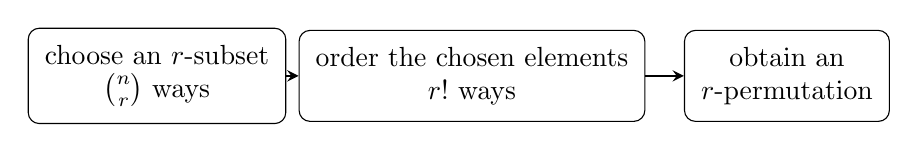
\begin{tikzpicture}[>=stealth, node distance=2.8cm]
    \node[draw, rounded corners, align=center, inner sep=6pt] (A) {choose an $r$-subset\\$\binom{n}{r}$ ways};
    \node[draw, rounded corners, align=center, inner sep=6pt, right of=A, xshift=1.2cm] (B) {order the chosen elements\\$r!$ ways};
    \node[draw, rounded corners, align=center, inner sep=6pt, right of=B, xshift=1.2cm] (C) {obtain an\\$r$-permutation};
    \draw[->, thick] (A) -- (B);
    \draw[->, thick] (B) -- (C);
\end{tikzpicture}
\end{center}

\begin{theorem}{Formula for combinations}{comb-formula}
For integers $n$ and $r$ with $0\le r\le n$,
\[
\binom{n}{r}=\frac{n!}{r!(n-r)!}.
\]
Equivalently,
\[
P(n,r)=\binom{n}{r}r!.
\]
\end{theorem}

\begin{proof}
Every $r$-permutation is obtained by first choosing an $r$-element subset and then ordering its $r$ elements. There are $\binom{n}{r}$ ways to choose the subset and $r!$ ways to order it. Hence
\[
P(n,r)=\binom{n}{r}r!.
\]
Using
\[
P(n,r)=\frac{n!}{(n-r)!},
\]
we obtain
\[
\binom{n}{r}=\frac{P(n,r)}{r!}=\frac{n!}{r!(n-r)!}.
\]
\end{proof}

\begin{keyformula}[title={Binomial coefficient formula}]
\[
\binom{n}{r}=\frac{n!}{r!(n-r)!}.
\]
Special cases:
\[
\binom{n}{0}=1,\qquad \binom{n}{1}=n,\qquad \binom{n}{n-1}=n,\qquad \binom{n}{n}=1.
\]
\end{keyformula}

\begin{extension}[title={Canonical choose-then-order decomposition}]
The identity
\[
P(n,r)=\binom{n}{r}r!
\]
is not just a formula. It describes the exact structure of an ordered selection: first determine \emph{which} elements appear, then determine \emph{in what order} they appear. This structural viewpoint is often more useful than memorising the factorial form directly.
\end{extension}

\begin{examplebox}[title={Bit strings with exactly $r$ ones}]
How many $0$-$1$ strings of length $n$ contain exactly $r$ ones?

\textbf{Solution.}
Such a string is completely determined by the positions of the $r$ ones. Hence we choose $r$ positions from the $n$ available positions, giving
\[
\binom{n}{r}
\]
strings.
\end{examplebox}

\begin{examplebox}[title={Selecting a team}]
There are $9$ boys and $11$ girls. How many ways are there to choose $3$ boys and $4$ girls to form a team?

\textbf{Solution.}
Choose the boys and girls independently:
\[
\binom{9}{3}\binom{11}{4}=84\cdot 330=27{,}720.
\]
\end{examplebox}

\begin{examplebox}[title={A required pair}]
Suppose two members $A$ and $B$ of a group of $12$ insist on working as a pair: any $5$-person team must contain either both or neither. How many such teams are possible?

\textbf{Solution.}
There are two disjoint cases.
\begin{itemize}[leftmargin=*]
    \item Both $A$ and $B$ are included: choose the remaining $3$ members from the other $10$, giving $\binom{10}{3}$ teams.
    \item Neither $A$ nor $B$ is included: choose all $5$ members from the other $10$, giving $\binom{10}{5}$ teams.
\end{itemize}
Therefore the total number is
\[
\binom{10}{3}+\binom{10}{5}=120+252=372.
\]
\end{examplebox}

\begin{examplebox}[title={Powerball}]
In Powerball, five regular numbers are chosen from $1$ to $69$, and one special Powerball number is chosen from $1$ to $26$. How many tickets are possible?

\textbf{Solution.}
The five regular numbers form an unordered selection of $5$ distinct integers from $69$, so there are $\binom{69}{5}$ possibilities. The Powerball is then chosen in $26$ ways. Hence the total number of tickets is
\[
\binom{69}{5}\cdot 26=292{,}201{,}338.
\]
\end{examplebox}

\begin{examplebox}[title={Poker hands}]
How many $5$-card poker hands can be dealt from a standard deck of $52$ cards?

\textbf{Solution.}
A hand is an unordered selection of $5$ cards from $52$, so the number of hands is
\[
\binom{52}{5}=2{,}598{,}960.
\]
\end{examplebox}

\subsubsection{Symmetry of binomial coefficients}

\begin{theorem}{Symmetry identity}{comb-symmetry}
For integers $n$ and $r$ with $0\le r\le n$,
\[
\binom{n}{r}=\binom{n}{n-r}.
\]
\end{theorem}

\begin{proof}
Using the factorial formula,
\[
\binom{n}{r}=\frac{n!}{r!(n-r)!}=\frac{n!}{(n-r)![n-(n-r)]!}=\binom{n}{n-r}.
\]
\end{proof}

\begin{extension}[title={Combinatorial meaning of the symmetry}]
Choosing $r$ objects to include is equivalent to choosing the $n-r$ objects to exclude. This gives a direct bijection between $r$-subsets and $(n-r)$-subsets: send each subset to its complement.
\end{extension}

\begin{commonmistake}[title={Combination formulas are for unordered selections only}]
A formula such as $\binom{n}{r}$ should not be used unless different orderings of the same chosen elements represent the \emph{same} object. Cards in a hand form a combination; prize winners with distinct ranks form a permutation.
\end{commonmistake}

%==================================================
\subsection{Combinatorial Proof}
%==================================================

\begin{definition}{Combinatorial proof}{comb-proof}
A \emph{combinatorial proof} of an identity is a proof that interprets both sides of the identity as counting the same set of objects in two different ways.
\end{definition}

The point is not algebraic manipulation. Instead, one identifies one collection of objects and counts it by two valid descriptions.

\begin{examplebox}[title={Pascal identity}]
Prove that for integers $n\ge k\ge 1$,
\[
\binom{n}{k}=\binom{n-1}{k}+\binom{n-1}{k-1}.
\]

\textbf{Combinatorial proof.}
Count the number of $k$-element subsets of an $n$-element set containing a distinguished element $x$ or not containing $x$.

Let the ground set be
\[
S=\{x\}\cup T,
\qquad |T|=n-1.
\]
The left-hand side counts all $k$-element subsets of $S$, so it equals $\binom{n}{k}$.

Now partition these subsets into two disjoint classes:
\begin{itemize}[leftmargin=*]
    \item subsets not containing $x$: choose all $k$ elements from $T$, giving $\binom{n-1}{k}$ choices;
    \item subsets containing $x$: then the remaining $k-1$ elements are chosen from $T$, giving $\binom{n-1}{k-1}$ choices.
\end{itemize}
Adding the disjoint cases gives
\[
\binom{n}{k}=\binom{n-1}{k}+\binom{n-1}{k-1}.
\]
\end{examplebox}

\begin{examplebox}[title={An equality of two partition counts}]
Show that the number of ways to write
\[
n=a+b
\qquad\text{with}\qquad a\ge b\ge 0
\]
is equal to the number of ways to write
\[
n=c+2d
\qquad\text{with}\qquad c,d\ge 0.
\]

\textbf{Combinatorial proof.}
Given a representation $n=a+b$ with $a\ge b\ge 0$, define
\[
c=a-b,\qquad d=b.
\]
Then
\[
c+2d=(a-b)+2b=a+b=n,
\]
and $c,d\ge 0$. Conversely, given $n=c+2d$ with $c,d\ge 0$, set
\[
a=c+d,\qquad b=d.
\]
Then
\[
a+b=(c+d)+d=c+2d=n,
\qquad a\ge b\ge 0.
\]
These constructions are inverse to each other, so they define a bijection between the two families of representations. Therefore the two counts are equal.
\end{examplebox}

\begin{extension}[title={How to invent a combinatorial proof}]
A useful template is:
\begin{enumerate}[leftmargin=*]
    \item decide what set of objects one side is naturally counting;
    \item check whether the other side counts the same set after partitioning, reordering, or re-encoding the objects;
    \item make the two counting viewpoints explicit.
\end{enumerate}
In many binomial identities, the right side arises by partitioning the same family into disjoint cases.
\end{extension}

%==================================================
\subsection{Special Techniques}
%==================================================

\subsubsection*{1. Worst-case construction for pigeonhole problems}
To determine the smallest number that guarantees a repetition or threshold occupancy, first maximise how many objects can be placed while still \emph{avoiding} the desired conclusion. Then add one more object.

\subsubsection*{2. Average-occupancy interpretation}
When using the generalized pigeonhole principle, compute
\[
\left\lceil \frac{N}{k}\right\rceil
\]
and interpret it as the minimum guaranteed size of the most populated box.

\subsubsection*{3. Choose-then-order}
To count ordered selections, it is often efficient to first choose the participating elements and then order them:
\[
P(n,r)=\binom{n}{r}r!.
\]
This is especially useful when a question mixes unordered selection with labelled roles.

\subsubsection*{4. Block method in permutations}
When specified objects must stay together, compress them into a single block. If the internal order is flexible, multiply by the number of internal block arrangements afterward.

\subsubsection*{5. Convert exact-content questions into position choices}
Questions such as ``exactly $r$ ones'' are often best solved by choosing positions rather than building strings directly.

\subsubsection*{6. Prove identities by counting one set in two ways}
For combinatorial proof, do not start with algebra. Start by asking: \emph{what family of objects could both sides be counting?}

\begin{examtip}[title={High-yield diagnostic checklist}]
Before finalising a solution from this handout, verify:
\begin{enumerate}[leftmargin=*]
    \item Have I identified the boxes correctly in the pigeonhole model?
    \item Have I decided correctly whether order matters?
    \item If I used $\binom{n}{r}$, did I justify why the selection is unordered?
    \item If I used $P(n,r)$, did I account for distinct roles or positions?
    \item If I wrote a combinatorial proof, did both sides count the same set of objects?
\end{enumerate}
\end{examtip}

%==================================================
\subsection{Summary Table}
%==================================================

\begin{center}
\small
\begin{tabular}{@{}p{0.25\textwidth}p{0.25\textwidth}p{0.38\textwidth}@{}}
\toprule
\textbf{Problem type} & \textbf{Main tool} & \textbf{Typical signal} \\
\midrule
forced repetition / collision & pigeonhole principle & more objects than categories \\
minimum guaranteed occupancy & generalized pigeonhole principle & distribute $N$ objects among $k$ boxes \\
ordered selection of $r$ distinct objects & $P(n,r)$ & rank, arrange, first/second/third, line up \\
unordered selection of $r$ objects & $\binom{n}{r}$ & choose, committee, hand, team \\
identity of counting expressions & combinatorial proof & prove two formulas are equal by interpretation \\
\bottomrule
\end{tabular}
\end{center}

\begin{commonmistake}[title={Final distinction to remember}]
The expressions
\[
P(n,r),\qquad \binom{n}{r},\qquad \left\lceil\frac{N}{k}\right\rceil
\]
solve fundamentally different kinds of problems. A large fraction of exam errors in this handout come from selecting the correct formula too early, before deciding whether the problem is about forcing, ordering, or unordered choice.
\end{commonmistake}}{}
\IfFileExists{chapters/handout03.tex}{\part{Counting}
\section{Handout 03: Binomial Theorem, Generalized Permutations and Combinations}

\subsection{Overview}

This handout completes Part~I on counting by introducing three major ideas:
\begin{itemize}[leftmargin=*]
    \item the \emph{binomial theorem} and basic binomial identities;
    \item the \emph{division rule}, which is the standard way to remove systematic overcounting;
    \item generalized counting models involving
    \begin{itemize}[leftmargin=*]
        \item cyclic arrangements,
        \item repetition,
        \item indistinguishable objects,
        \item distributions into boxes.
    \end{itemize}
\end{itemize}

The main exam skill in this handout is to distinguish among the following situations:
\[
\begin{aligned}
&\text{ordered vs unordered}, &&
\text{with repetition vs without repetition},\\
&\text{distinguishable vs indistinguishable}, &&
\text{linear vs cyclic}.
\end{aligned}
\]

\begin{examtip}[title={Main modelling checklist for Handout 03}]
Before writing any formula, decide all four of the following:
\begin{enumerate}[leftmargin=*]
    \item Does order matter?
    \item Is repetition allowed?
    \item Are equal-looking objects actually indistinguishable?
    \item Are two arrangements identified by rotation?
\end{enumerate}
Most errors in this handout come from answering one of these four questions incorrectly.
\end{examtip}

%==================================================
\subsection{The Binomial Theorem}
%==================================================

\begin{theorem}{Binomial Theorem}{binomial-theorem}
Let $x$ and $y$ be variables and let $n$ be a nonnegative integer. Then
\[
(x+y)^n
=
\sum_{i=0}^{n}\binom{n}{i}x^{\,n-i}y^i.
\]
Equivalently,
\[
(x+y)^n
=
\binom{n}{0}x^n+\binom{n}{1}x^{n-1}y+\cdots+\binom{n}{n-1}xy^{n-1}+\binom{n}{n}y^n.
\]
\end{theorem}

\begin{proof}
Expand
\[
(x+y)^n=(x+y)(x+y)\cdots(x+y)
\]
as a product of $n$ identical factors. A term of the form
\[
x^{n-i}y^i
\]
arises precisely when one chooses $y$ from exactly $i$ of the $n$ factors, and therefore $x$ from the remaining $n-i$ factors. The number of such choices is
\[
\binom{n}{i}.
\]
Hence the coefficient of $x^{n-i}y^i$ is $\binom{n}{i}$, giving the formula.
\end{proof}

\begin{keyformula}[title={Binomial theorem}]
\[
(x+y)^n=\sum_{i=0}^{n}\binom{n}{i}x^{\,n-i}y^i.
\]
\end{keyformula}

\subsubsection{Coefficient extraction}

A binomial expansion question is often a coefficient question. One identifies the exponent pattern first, then determines which index $i$ is required.

\begin{examplebox}[title={Expansion of $(x+y)^4$}]
By the binomial theorem,
\[
(x+y)^4
=
\sum_{i=0}^{4}\binom{4}{i}x^{4-i}y^i
=
x^4+4x^3y+6x^2y^2+4xy^3+y^4.
\]
\end{examplebox}

\begin{examplebox}[title={Coefficient of $x^{12}y^{13}$ in $(x+y)^{25}$}]
In the general term
\[
\binom{25}{i}x^{25-i}y^i,
\]
we require
\[
25-i=12,\qquad i=13.
\]
Hence the coefficient is
\[
\binom{25}{13}=\frac{25!}{13!12!}=5{,}200{,}300.
\]
\end{examplebox}

\begin{examplebox}[title={Coefficient of $x^{12}y^{13}$ in $(2x-3y)^{25}$}]
Using the binomial theorem with $2x$ in place of $x$ and $-3y$ in place of $y$,
\[
(2x-3y)^{25}
=
\sum_{i=0}^{25}\binom{25}{i}(2x)^{25-i}(-3y)^i.
\]
To obtain $x^{12}y^{13}$, we again take $i=13$. Therefore the coefficient is
\[
\binom{25}{13}2^{12}(-3)^{13}.
\]
\end{examplebox}

\begin{commonmistake}[title={Coefficient questions with scaled variables}]
In expressions such as $(2x-3y)^n$, the coefficient is \emph{not} just a binomial coefficient. One must also include the powers of the numerical multipliers and the sign.
\end{commonmistake}

\begin{extension}[title={Why the coefficient is a combination}]
The coefficient of $x^{n-i}y^i$ counts the number of ways to choose exactly which $i$ factors contribute the $y$ term. This is why binomial coefficients appear naturally: every monomial in the expansion corresponds to a subset of the $n$ factor positions.
\end{extension}

%==================================================
\subsection{Basic Binomial Identities}
%==================================================

\begin{theorem}{Sum of the binomial coefficients}{sum-binomial}
For every nonnegative integer $n$,
\[
\sum_{i=0}^{n}\binom{n}{i}=2^n.
\]
\end{theorem}

\begin{proof}
Substitute $x=1$ and $y=1$ into the binomial theorem:
\[
2^n=(1+1)^n=\sum_{i=0}^{n}\binom{n}{i}1^{n-i}1^i=\sum_{i=0}^{n}\binom{n}{i}.
\]
\end{proof}

\begin{examplebox}[title={Combinatorial meaning of $\sum_{i=0}^{n}\binom{n}{i}=2^n$}]
Let $S$ be an $n$-element set. The quantity $2^n$ counts all subsets of $S$. On the other hand, for each $i$ there are $\binom{n}{i}$ subsets of size $i$. Summing over all possible sizes gives
\[
\sum_{i=0}^{n}\binom{n}{i}=2^n.
\]
\end{examplebox}

\begin{theorem}{Pascal's Identity}{pascal-identity}
For integers $n\ge r\ge 1$,
\[
\binom{n+1}{r}=\binom{n}{r}+\binom{n}{r-1}.
\]
\end{theorem}

\begin{proof}
Count the $r$-element subsets of an $(n+1)$-element set $S$. Fix one distinguished element $a\in S$, and let $T=S\setminus\{a\}$, so $|T|=n$.

Every $r$-element subset of $S$ falls into exactly one of two disjoint classes:
\begin{itemize}[leftmargin=*]
    \item those that do not contain $a$, of which there are $\binom{n}{r}$;
    \item those that contain $a$, in which case the remaining $r-1$ elements must be chosen from $T$, giving $\binom{n}{r-1}$.
\end{itemize}
Adding the two disjoint classes gives
\[
\binom{n+1}{r}=\binom{n}{r}+\binom{n}{r-1}.
\]
\end{proof}

% Pascal triangle fragment illustrating Pascal's identity row-by-row
\begin{center}
\begin{tikzpicture}[x=1cm,y=0.65cm]
\node at (0,0) {$1$};
\node at (-0.5,-1) {$1$}; \node at (0.5,-1) {$1$};
\node at (-1,-2) {$1$}; \node at (0,-2) {$2$}; \node at (1,-2) {$1$};
\node at (-1.5,-3) {$1$}; \node at (-0.5,-3) {$3$}; \node at (0.5,-3) {$3$}; \node at (1.5,-3) {$1$};
\node at (-2,-4) {$1$}; \node at (-1,-4) {$4$}; \node at (0,-4) {$6$}; \node at (1,-4) {$4$}; \node at (2,-4) {$1$};
\draw[->,gray] (-1,-2.4) -- (-0.15,-3.6);
\draw[->,gray] (0,-2.4) -- (-0.15,-3.6);
\end{tikzpicture}
\end{center}

\begin{extension}[title={Structural meaning of Pascal's identity}]
Pascal's identity is a prototype of a counting argument by partition. The right-hand side arises by splitting a family of subsets into two disjoint classes according to whether a distinguished element is present.
\end{extension}

%==================================================
\subsection{Division Rule}
%==================================================

The division rule is the standard tool for correcting uniform overcounting.

\begin{definition}{A $k$-to-$1$ function}{k-to-1}
A function $f:X\to Y$ is called \emph{$k$-to-$1$} if for every $y\in Y$, there are exactly $k$ elements $x\in X$ such that
\[
f(x)=y.
\]
\end{definition}

\begin{theorem}{Division Rule}{division-rule}
If $f:X\to Y$ is a $k$-to-$1$ function between finite sets, then
\[
|Y|=\frac{|X|}{k}.
\]
\end{theorem}

\begin{proof}
Because every element of $Y$ has exactly $k$ preimages, the set $X$ is partitioned into $|Y|$ disjoint fibres, each of size $k$. Hence
\[
|X|=k|Y|,
\]
and therefore
\[
|Y|=\frac{|X|}{k}.
\]
\end{proof}

\begin{keyformula}[title={Division rule}]
\[
\text{If a known set }X\text{ maps }k\text{-to-}1\text{ onto }Y,\text{ then }|Y|=\frac{|X|}{k}.
\]
\end{keyformula}

\begin{examtip}[title={When the division rule appears}]
Use the division rule whenever several linear descriptions represent the same final object. The main task is then to determine the overcounting factor $k$ exactly.
\end{examtip}

%==================================================
\subsection{Permutations Around a Cycle}
%==================================================

A cyclic arrangement identifies linear orders that differ only by rotation.

\begin{theorem}{Cyclic $r$-permutations}{cycle-permutation}
The number of ways to choose $r$ elements from an $n$-element set and arrange them around a cycle is
\[
\frac{1}{r}P(n,r)=\frac{n!}{r(n-r)!}.
\]
\end{theorem}

\begin{proof}
Let $P$ be the set of all linear $r$-permutations of the given $n$-element set, so
\[
|P|=P(n,r).
\]
Let $C$ be the set of cyclic arrangements of $r$ distinct chosen elements.

Define a map
\[
f:P\to C
\]
by sending a linear arrangement $(a_1,a_2,\dots,a_r)$ to the corresponding cyclic arrangement with the same circular order.

For a fixed cyclic arrangement, there are exactly $r$ linear arrangements mapping to it, namely the $r$ cyclic shifts
\[
(a_1,a_2,\dots,a_r),\ (a_2,a_3,\dots,a_r,a_1),\ \dots,\ (a_r,a_1,\dots,a_{r-1}).
\]
Hence $f$ is $r$-to-$1$. By the division rule,
\[
|C|=\frac{|P|}{r}=\frac{P(n,r)}{r}=\frac{n!}{r(n-r)!}.
\]
\end{proof}

% Cyclic arrangement equivalence under rotation
\begin{center}
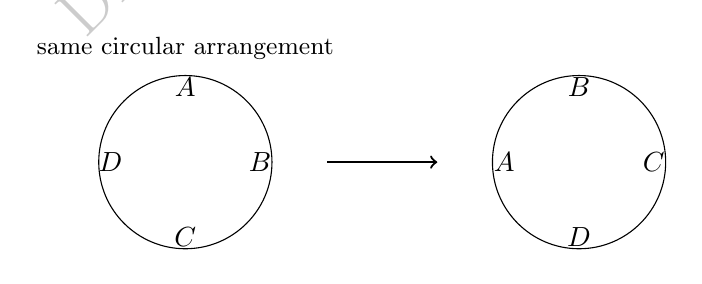
\begin{tikzpicture}[scale=1]
\draw (0,0) circle (1.1);
\node at (0,1.45) {\small same circular arrangement};
\node at (0,0.95) {$A$};
\node at (0.95,0) {$B$};
\node at (0,-0.95) {$C$};
\node at (-0.95,0) {$D$};

\draw[->,thick] (1.8,0) -- (3.2,0);

\draw (5,0) circle (1.1);
\node at (5,0.95) {$B$};
\node at (5.95,0) {$C$};
\node at (5,-0.95) {$D$};
\node at (4.05,0) {$A$};
\end{tikzpicture}
\end{center}

\begin{examplebox}[title={Three students around a table}]
The number of ways to seat $3$ students around a round table is
\[
\frac{P(3,3)}{3}=\frac{3!}{3}=2.
\]
Thus there are exactly two cyclic arrangements.
\end{examplebox}

\begin{examplebox}[title={Choosing and seating $r$ students around a round table}]
If one must choose $r$ students from $n$ and then seat them around a round table, the answer is
\[
\frac{1}{r}P(n,r)=\frac{n!}{r(n-r)!}.
\]
This is the direct application of the theorem above.
\end{examplebox}

\begin{commonmistake}[title={Linear order versus cyclic order}]
For a linear arrangement, different starting positions matter; for a cyclic arrangement, they do not. Dividing by $r$ is valid only because all $r$ chosen elements are distinct and every cyclic arrangement has exactly $r$ linear representatives.
\end{commonmistake}

\begin{extension}[title={Division by symmetry}]
The factor $r$ arises from rotational symmetry. More generally, whenever a symmetry group acts freely on a set of linear descriptions, the number of genuinely different configurations is obtained by dividing by the orbit size.
\end{extension}

%==================================================
\subsection{Permutations With Repetition}
%==================================================

\begin{theorem}{$r$-permutations with repetition}{perm-with-repetition}
The number of ordered strings of length $r$ formed from a set of $n$ elements, when repetition is allowed, is
\[
n^r.
\]
\end{theorem}

\begin{proof}
Each of the $r$ positions may be filled independently with any of the $n$ available elements. By the product rule, the total number of strings is
\[
\underbrace{n\cdot n\cdots n}_{r\text{ times}}=n^r.
\]
\end{proof}

\begin{keyformula}[title={Ordered selection with repetition}]
\[
\text{number of length-}r\text{ strings from }n\text{ symbols}=n^r.
\]
\end{keyformula}

\begin{examplebox}[title={Strings over the English alphabet}]
The number of strings of length $r$ formed from the English alphabet is
\[
26^r,
\]
since each of the $r$ positions has $26$ choices.
\end{examplebox}

\begin{examplebox}[title={Four-digit PIN code}]
If digits may repeat, then a four-digit PIN code has
\[
10^4=10{,}000
\]
possible ordered strings.
\end{examplebox}

%==================================================
\subsection{Combinations With Repetition}
%==================================================

Here order does not matter, but repetition is allowed.

\begin{theorem}{$r$-combinations with repetition}{comb-with-repetition}
The number of $r$-combinations from a set with $n$ elements, when repetition is allowed, is
\[
\binom{n+r-1}{r}=\binom{n+r-1}{n-1}.
\]
\end{theorem}

\begin{proof}
Interpret an $r$-combination with repetition as distributing $r$ indistinguishable balls into $n$ distinguishable bins, where the $i$-th bin records how many copies of the $i$-th element are chosen.

Represent such a distribution by a string consisting of
\[
r\text{ balls }(\bullet)\quad\text{and}\quad n-1\text{ dividers }(|).
\]
For example, the string
\[
\bullet\bullet\,|\,|\,\bullet\,|\,\bullet
\]
with $n=4$ and $r=4$ corresponds to the multiset containing $2$ copies of the first element, $0$ copies of the second, $1$ copy of the third, and $1$ copy of the fourth.

Thus every $r$-combination with repetition corresponds bijectively to a string of length
\[
r+(n-1)=n+r-1
\]
containing $r$ balls and $n-1$ dividers. Such a string is determined by choosing the positions of the $r$ balls (or, equivalently, the $n-1$ dividers). Hence the number of such strings is
\[
\binom{n+r-1}{r}=\binom{n+r-1}{n-1}.
\]
\end{proof}

\begin{keyformula}[title={Unordered selection with repetition}]
\[
\text{number of }r\text{-combinations from }n\text{ elements with repetition}
=
\binom{n+r-1}{r}.
\]
\end{keyformula}

% Stars and bars representation for a multiset selection
\begin{center}
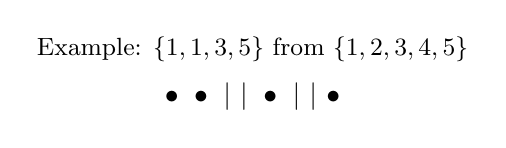
\begin{tikzpicture}[x=0.5cm,y=0.5cm]
\node at (0,1.2) {\small Example: $\{1,1,3,5\}$ from $\{1,2,3,4,5\}$};
\node at (0,0) {$\bullet\ \bullet\ |\ |\ \bullet\ |\ |\ \bullet$};
\end{tikzpicture}
\end{center}

\begin{examplebox}[title={Selecting fruit}]
How many ways are there to select $3$ pieces of fruit from a bowl containing apples, oranges, and pears, if order does not matter?

\textbf{Solution.}
This is a $3$-combination from a set of $3$ fruit types with repetition allowed. Hence the answer is
\[
\binom{3+3-1}{3}=\binom{5}{3}=10.
\]
\end{examplebox}

\begin{examplebox}[title={Cookie shop}]
A cookie shop offers $4$ kinds of cookies. The number of ways to choose $6$ cookies, if order does not matter, is
\[
\binom{4+6-1}{6}=\binom{9}{6}=84.
\]
\end{examplebox}

\subsubsection{Nonnegative integer solutions}

The stars-and-bars theorem is equivalent to counting nonnegative integer solutions.

\begin{theorem}{Nonnegative solutions of a linear equation}{nonnegative-solutions}
The number of solutions in nonnegative integers to
\[
x_1+x_2+\cdots+x_n=r
\]
is
\[
\binom{n+r-1}{r}.
\]
\end{theorem}

\begin{proof}
A solution $(x_1,\dots,x_n)$ specifies how many of the $r$ indistinguishable objects are placed into each of the $n$ labelled bins. This is precisely the same model as $r$-combinations with repetition from an $n$-element set, so the answer is
\[
\binom{n+r-1}{r}.
\]
\end{proof}

\begin{examplebox}[title={Equation $x_1+x_2+x_3=11$}]
The number of nonnegative integer solutions of
\[
x_1+x_2+x_3=11
\]
is
\[
\binom{3+11-1}{11}=\binom{13}{11}=\binom{13}{2}=78.
\]
\end{examplebox}

\begin{examplebox}[title={Lower bounds by shifting variables}]
How many integer solutions are there to
\[
x_1+x_2+x_3=11,
\qquad
x_1\ge 1,\ x_2\ge 2,\ x_3\ge 3?
\]

\textbf{Solution.}
Write
\[
x_1=1+y_1,\qquad x_2=2+y_2,\qquad x_3=3+y_3,
\]
where $y_1,y_2,y_3\ge 0$. Then
\[
y_1+y_2+y_3=11-(1+2+3)=5.
\]
Hence the number of solutions is
\[
\binom{3+5-1}{5}=\binom{7}{5}=\binom{7}{2}=21.
\]
\end{examplebox}

\begin{extension}[title={Canonical stars-and-bars encoding}]
The stars-and-bars argument is a canonical bijection: a multiset choice is fully determined by the multiplicity of each symbol, and these multiplicities are encoded by block lengths between dividers. This is why the same formula also counts nonnegative integer solutions.
\end{extension}

\begin{commonmistake}[title={Repetition allowed does not mean order matters}]
The formulas
\[
n^r
\qquad\text{and}\qquad
\binom{n+r-1}{r}
\]
both involve repetition, but they count different objects. The first counts ordered strings; the second counts unordered selections.
\end{commonmistake}

%==================================================
\subsection{Permutations With Indistinguishable Objects}
%==================================================

\begin{theorem}{Permutations of indistinguishable objects}{indistinguishable-perm}
Suppose there are $n$ objects in total, with
\[
n_1\text{ objects of type }1,\quad
n_2\text{ objects of type }2,\quad
\dots,\quad
n_k\text{ objects of type }k,
\]
where
\[
n_1+n_2+\cdots+n_k=n.
\]
Then the number of distinct permutations is
\[
\frac{n!}{n_1!n_2!\cdots n_k!}.
\]
\end{theorem}

\begin{proof}
First pretend that all objects are distinguishable. Then there are $n!$ linear permutations.

Now pass to the setting in which objects of the same type are indistinguishable. Different labelings of the identical objects produce the same final arrangement. For each final arrangement, the objects of type $1$ can be internally relabelled in $n_1!$ ways, those of type $2$ in $n_2!$ ways, and so on. Hence every distinct arrangement is represented exactly
\[
n_1!n_2!\cdots n_k!
\]
times among the $n!$ labelled permutations.

By the division rule, the number of distinct permutations is
\[
\frac{n!}{n_1!n_2!\cdots n_k!}.
\]
\end{proof}

\begin{keyformula}[title={Indistinguishable objects}]
\[
\text{number of distinct permutations}
=
\frac{n!}{n_1!n_2!\cdots n_k!}.
\]
\end{keyformula}

\begin{examplebox}[title={The word SUCCESS}]
The word \texttt{SUCCESS} has $7$ letters with multiplicities
\[
S^3,\quad C^2,\quad U^1,\quad E^1.
\]
Hence the number of distinct rearrangements is
\[
\frac{7!}{3!2!1!1!}=420.
\]
\end{examplebox}

\begin{examplebox}[title={The word MISSISSIPPI}]
The word \texttt{MISSISSIPPI} has $11$ letters with multiplicities
\[
I^4,\quad S^4,\quad P^2,\quad M^1.
\]
Therefore the number of distinct rearrangements is
\[
\frac{11!}{4!4!2!1!}=34{,}650.
\]
\end{examplebox}

\begin{extension}[title={Label-then-divide strategy}]
A reliable way to count with indistinguishable objects is:
\begin{enumerate}[leftmargin=*]
    \item temporarily label identical objects so that everything becomes distinguishable;
    \item count the labelled arrangements;
    \item divide by the number of relabellings that do not change the final visible arrangement.
\end{enumerate}
This is one of the most useful recurring patterns in advanced counting.
\end{extension}

%==================================================
\subsection{Distributions Into Boxes}
%==================================================

\subsubsection{Distinguishable objects into distinguishable boxes}

\begin{theorem}{Specified occupancy distribution}{box-distribution}
The number of ways to distribute $n$ distinguishable objects into $k$ distinguishable boxes so that box $1$ receives $n_1$ objects, box $2$ receives $n_2$ objects, \dots, box $k$ receives $n_k$ objects, where
\[
n_1+n_2+\cdots+n_k=n,
\]
is
\[
\frac{n!}{n_1!n_2!\cdots n_k!}.
\]
\end{theorem}

\begin{proof}
Choose which $n_1$ objects go to box $1$, then which $n_2$ of the remaining objects go to box $2$, and so on. The count is
\[
\binom{n}{n_1}\binom{n-n_1}{n_2}\cdots \binom{n-n_1-\cdots-n_{k-1}}{n_k}.
\]
Simplifying this product yields
\[
\frac{n!}{n_1!n_2!\cdots n_k!}.
\]
\end{proof}

\begin{examplebox}[title={Distribution with fixed box sizes}]
The number of ways to distribute $8$ distinct objects into $3$ distinct boxes so that the box sizes are $3,2,3$ is
\[
\frac{8!}{3!2!3!}=560.
\]
\end{examplebox}

\subsubsection{Indistinguishable objects into distinguishable boxes}

If the objects are indistinguishable and the boxes are distinguishable, one is counting nonnegative integer solutions.

\begin{examplebox}[title={Five indistinguishable objects into three distinguishable boxes}]
The number of ways to distribute $5$ indistinguishable objects into $3$ distinguishable boxes is the number of nonnegative integer solutions of
\[
x_1+x_2+x_3=5.
\]
Hence the answer is
\[
\binom{3+5-1}{5}=\binom{7}{5}=\binom{7}{2}=21.
\]
\end{examplebox}

\subsubsection{Optional viewpoints from the handout}

\begin{extension}[title={Distinguishable objects into indistinguishable boxes}]
When the boxes are indistinguishable, there is generally no similarly simple closed formula. The handout treats this by breaking into cases and, optionally, via Stirling numbers of the second kind:
\[
S(n,j)=\frac{1}{j!}\sum_{i=0}^{j-1}(-1)^i\binom{j}{i}(j-i)^n.
\]
These count the ways to distribute $n$ distinguishable objects into $j$ indistinguishable nonempty boxes.
\end{extension}

\begin{extension}[title={Indistinguishable objects into indistinguishable boxes}]
This becomes a partition problem. The number of ways to distribute $n$ indistinguishable objects into at most $k$ indistinguishable boxes is the number of partitions of $n$ into at most $k$ positive parts, often denoted by $p_k(n)$.
\end{extension}

%==================================================
\subsection{Special Techniques}
%==================================================

\subsubsection*{1. Coefficient targeting in binomial expansions}
When asked for a specific coefficient, match exponents first. Only after identifying the correct index should you substitute the associated binomial coefficient and numerical multipliers.

\subsubsection*{2. Count first, then divide}
If many linear descriptions represent the same final object, count the linear descriptions and divide by the uniform overcounting factor. This is the main mechanism behind cyclic permutations and indistinguishable objects.

\subsubsection*{3. Stars and bars}
Whenever the problem is about unordered selection with repetition, or nonnegative integer solutions to a sum equation, try to convert the problem into placing balls and dividers in a line.

\subsubsection*{4. Shift lower bounds away}
For constraints such as
\[
x_i\ge a_i,
\]
write
\[
x_i=a_i+y_i,\qquad y_i\ge 0,
\]
and reduce the problem to a standard nonnegative-solution count.

\subsubsection*{5. Label identical objects temporarily}
For problems involving repeated letters or identical objects, first pretend the copies are distinct, count all permutations, then divide by the internal relabellings.

\subsubsection*{6. Diagnose the symmetry}
If a problem involves round tables, necklaces, rotations, repeated letters, or any other visible identification of multiple linear arrangements, ask immediately whether the same visible arrangement is being counted several times.

\begin{examtip}[title={High-yield distinction table}]
A quick diagnostic:
\[
\begin{array}{c|c}
\text{Situation} & \text{Typical formula} \\ \hline
\text{ordered, no repetition} & P(n,r)=\dfrac{n!}{(n-r)!} \\
\text{ordered, repetition allowed} & n^r \\
\text{unordered, no repetition} & \binom{n}{r} \\
\text{unordered, repetition allowed} & \binom{n+r-1}{r} \\
\text{indistinguishable copies in a line} & \dfrac{n!}{n_1!\cdots n_k!} \\
\text{around a cycle} & \dfrac{P(n,r)}{r}
\end{array}
\]
Always verify that the modelling assumptions match the row you use.
\end{examtip}

%==================================================
\subsection{Summary Table}
%==================================================

\begin{center}
\scriptsize
\begin{tabular}{@{}p{0.28\textwidth}p{0.27\textwidth}p{0.27\textwidth}@{}}
\toprule
& \textbf{$r$-permutation} & \textbf{$r$-combination} \\
\midrule
without repetition
&
\[
P(n,r)=\frac{n!}{(n-r)!}
\]
&
\[
\binom{n}{r}=\frac{n!}{(n-r)!r!}
\]
\\[1.0em]
with repetition
&
\[
n^r
\]
&
\[
\binom{n+r-1}{r}
\]
\\[1.0em]
with indistinguishable objects
&
\[
\frac{n!}{n_1!n_2!\cdots n_k!}
\]
&
\text{use multiplicities / multiset model}
\\[1.0em]
around a cycle
&
\[
\frac{P(n,r)}{r}
=
\frac{n!}{r(n-r)!}
\]
&
\text{not a standard separate formula}
\\
\bottomrule
\end{tabular}
\end{center}

\begin{commonmistake}[title={Final warning for Handout 03}]
The formulas in this handout are similar in appearance but answer different questions. Never choose a formula just because it looks familiar. First classify the problem by order, repetition, indistinguishability, and cyclic symmetry; only then substitute a formula.
\end{commonmistake}
}{}
\IfFileExists{chapters/handout04.tex}{% Source reference: :contentReference[oaicite:0]{index=0}
\part{Recurrence Relations}
\section{Handout 04: Recurrence Relations}

\subsection{Overview}

This handout begins Part II of the course. The goal is not yet to develop the full theory for solving recurrence relations, but to learn how to \emph{model} a problem recursively.

A recurrence relation is useful when a problem of size $n$ can be reduced to one or more smaller problems, typically of sizes $n-1$, $n-2$, and so on. In this handout, the emphasis is on:
\begin{itemize}[leftmargin=*]
    \item understanding what a recurrence relation is;
    \item identifying the correct size parameter;
    \item deriving initial conditions;
    \item splitting a problem into exhaustive and non-overlapping cases;
    \item relating a counting problem of size $n$ to smaller instances.
\end{itemize}

The main examples are:
\begin{itemize}[leftmargin=*]
    \item Tower of Hanoi;
    \item compound interest;
    \item the graduate-student job problem and Fibonacci numbers;
    \item $0$-$1$ strings with no consecutive $0$'s;
    \item decimal codewords with an even number of zero digits.
\end{itemize}

\begin{examtip}[title={Main objective of Handout 04}]
For this handout, the central task is usually not ``solve the recurrence completely'' but rather ``derive the correct recurrence and initial conditions.'' A recurrence is only useful if the state variable is defined precisely.
\end{examtip}

%==================================================
\subsection{What Is a Recurrence Relation?}
%==================================================

\begin{definition}{Recurrence relation and initial conditions}{recurrence-def}
A \emph{recurrence relation} for a sequence $(a_n)$ is an equation that expresses $a_n$ in terms of one or more earlier terms of the sequence.

The accompanying \emph{initial conditions} specify enough starting values to determine the sequence uniquely.
\end{definition}

A recurrence model usually has two parts:
\begin{enumerate}[leftmargin=*]
    \item define the quantity $a_n$ clearly in terms of the problem size $n$;
    \item relate the size-$n$ problem to smaller instances.
\end{enumerate}

\begin{keyformula}[title={Core modelling pattern}]
\[
\text{current value} = \text{contribution from smaller cases}.
\]
A valid recurrence model must also include initial conditions.
\end{keyformula}

\begin{examplebox}[title={A simple financial example}]
If $P_n$ denotes the amount in an account after $n$ years and the balance grows by $11\%$ each year, then
\[
P_n=1.11P_{n-1}
\]
with initial condition
\[
P_0=10{,}000.
\]
The recurrence comes from the rule that each year's balance is the previous year's balance plus $11\%$ of the previous year's balance.
\end{examplebox}

\begin{commonmistake}[title={A recurrence without initial conditions is incomplete}]
The formula
\[
a_n=a_{n-1}+a_{n-2}
\]
does not determine a unique sequence by itself. Different initial conditions produce different sequences.
\end{commonmistake}

%==================================================
\subsection{Idea of Recurrence}
%==================================================

The key idea is to solve a large problem by reducing it to smaller ones. For a problem parameterized by $n$, we try to answer:
\begin{center}
\emph{How can the size-$n$ case be built from cases of smaller size?}
\end{center}

Typical strategies include:
\begin{itemize}[leftmargin=*]
    \item removing the last object or last step;
    \item splitting according to the last symbol or first symbol;
    \item separating what is already present from what is newly created;
    \item introducing extra states when one variable does not capture enough information.
\end{itemize}

\begin{extension}[title={Recurrence modelling is structural, not computational}]
A good recurrence is obtained by understanding the \emph{structure} of the objects being counted. The equation is a consequence of that structure; it is not something guessed from a few numerical values.
\end{extension}

%==================================================
\subsection{Example: Tower of Hanoi}
%==================================================

Let $H_n$ denote the minimum number of moves needed to transfer $n$ disks from one bar to another, subject to the rules:
\begin{enumerate}[leftmargin=*]
    \item only one disk may be moved at a time;
    \item no disk may be placed on top of a smaller disk.
\end{enumerate}

\begin{examplebox}[title={Tower of Hanoi recurrence}]
Define $H_n$ to be the minimum number of moves required to transfer $n$ disks from one peg to another.

The initial condition is
\[
H_1=1.
\]

To move $n$ disks:
\begin{enumerate}[leftmargin=*]
    \item move the top $n-1$ disks to the spare peg: $H_{n-1}$ moves;
    \item move the largest disk: $1$ move;
    \item move the $n-1$ disks onto the largest disk: $H_{n-1}$ moves.
\end{enumerate}
Hence
\[
H_n=2H_{n-1}+1
\qquad (n\ge 2).
\]
\end{examplebox}

% Tower of Hanoi decomposition: move n-1, move largest, move n-1 again.
\begin{center}
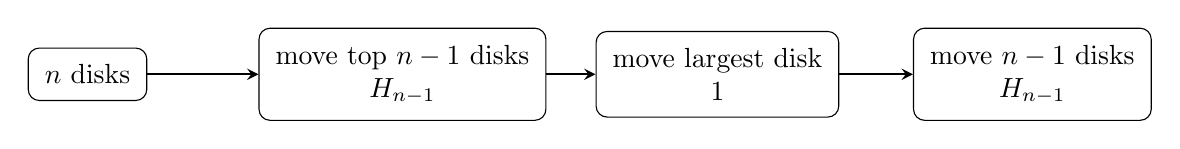
\begin{tikzpicture}[>=stealth]
    \node[draw,rounded corners,align=center,inner sep=6pt] (A) at (0,0) {$n$ disks};
    \node[draw,rounded corners,align=center,inner sep=6pt] (B) at (4.0,0) {move top $n-1$ disks\\$H_{n-1}$};
    \node[draw,rounded corners,align=center,inner sep=6pt] (C) at (8.0,0) {move largest disk\\$1$};
    \node[draw,rounded corners,align=center,inner sep=6pt] (D) at (12.0,0) {move $n-1$ disks\\$H_{n-1}$};
    \draw[->,thick] (A) -- (B);
    \draw[->,thick] (B) -- (C);
    \draw[->,thick] (C) -- (D);
\end{tikzpicture}
\end{center}

One can compute the first few values:
\[
H_1=1,\quad H_2=3,\quad H_3=7,\quad H_4=15,\quad H_5=31.
\]
This suggests the closed form
\[
H_n=2^n-1.
\]
Indeed, this can be proved by induction:
\[
H_n=2H_{n-1}+1=2(2^{n-1}-1)+1=2^n-1.
\]

\begin{examtip}[title={Why this recurrence is natural}]
The largest disk can move only once the top $n-1$ disks have been cleared, and after that those $n-1$ disks must be rebuilt on top of it. This forces the decomposition
\[
H_n=H_{n-1}+1+H_{n-1}.
\]
\end{examtip}

\begin{extension}[title={Reve's puzzle}]
If there are $k\ge 4$ pegs instead of $3$, the problem becomes a much deeper one. The four-peg case was solved only recently, and the general closed-form problem for larger $k$ is far subtler than the classical three-peg recurrence.
\end{extension}

%==================================================
\subsection{Example: Compound Interest}
%==================================================

\begin{examplebox}[title={Compound interest recurrence}]
Suppose $10{,}000$ dollars are deposited into an account earning $11\%$ annual interest, compounded once per year. Let $P_n$ denote the amount after $n$ years.

Then
\[
P_0=10{,}000,
\qquad
P_n=P_{n-1}+0.11P_{n-1}=1.11P_{n-1}.
\]
Iterating gives
\[
P_1=1.11P_0,
\qquad
P_2=1.11P_1=(1.11)^2P_0,
\qquad
\dots,
\qquad
P_n=(1.11)^nP_0.
\]
Hence
\[
P_{30}=(1.11)^{30}\cdot 10{,}000\approx 228{,}922.97.
\]
\end{examplebox}

This example is important because the recurrence is immediate from the problem statement. It also shows that some recurrences are simple enough to solve by direct iteration.

\begin{commonmistake}[title={Confusing the recurrence with the final closed form}]
The recurrence
\[
P_n=1.11P_{n-1}
\]
is the model. The expression
\[
P_n=(1.11)^nP_0
\]
is a derived formula obtained by repeated substitution.
\end{commonmistake}

%==================================================
\subsection{Example: Graduate-Student Job Problem}
%==================================================

Consider the following model: each professor graduates one student every year who becomes a professor, except first-year professors, who graduate no students. Assume no retirements.

Let $f_n$ denote the number of professors in year $n$.

The initial values are
\[
f_0=0,\qquad f_1=1,\qquad f_2=1.
\]
The first few values are
\[
f_3=2,\qquad f_4=3,\qquad f_5=5.
\]

\begin{examplebox}[title={Graduate-student job recurrence}]
To count the professors in year $n$, split them into two groups:
\begin{itemize}[leftmargin=*]
    \item the professors already present in year $n-1$, contributing $f_{n-1}$;
    \item the new professors produced in year $n$, which come from those who were already beyond their first year in year $n-1$.
\end{itemize}
These new professors correspond exactly to the professors present in year $n-2$. Therefore
\[
f_n=f_{n-1}+f_{n-2}
\qquad (n\ge 2).
\]
\end{examplebox}

This is the Fibonacci recurrence. The sequence $(f_n)$ is therefore the Fibonacci sequence with the given initial conditions.

\begin{extension}[title={Same recurrence, different initial conditions}]
The recurrence
\[
a_n=a_{n-1}+a_{n-2}
\]
appears in many unrelated problems. What distinguishes one application from another is often the initial conditions. Later in this handout, the same recurrence will appear again in a string-counting problem.
\end{extension}

%==================================================
\subsection{Example: Bit Strings With No Consecutive Zeros}
%==================================================

Let $a_n$ denote the number of $0$-$1$ strings of length $n$ that do not contain two consecutive $0$'s.

The initial values are
\[
a_1=2
\qquad\text{(namely $0,1$)},
\qquad
 a_2=3
\qquad\text{(namely $01,10,11$)}.
\]

\begin{examplebox}[title={Recurrence for strings with no consecutive zeros}]
Consider a valid string of length $n$ and examine its last bit.

\textbf{Case 1:} The last bit is $1$.
Then the first $n-1$ bits may be any valid string of length $n-1$. Hence this case contributes
\[
a_{n-1}.
\]

\textbf{Case 2:} The last bit is $0$.
Then the $(n-1)$st bit must be $1$, so the first $n-2$ bits may be any valid string of length $n-2$. Hence this case contributes
\[
a_{n-2}.
\]

The two cases are disjoint and exhaustive, so
\[
a_n=a_{n-1}+a_{n-2}
\qquad (n\ge 3).
\]
\end{examplebox}

% Case split for the final bit in a valid binary string with no consecutive zeros.
\begin{center}
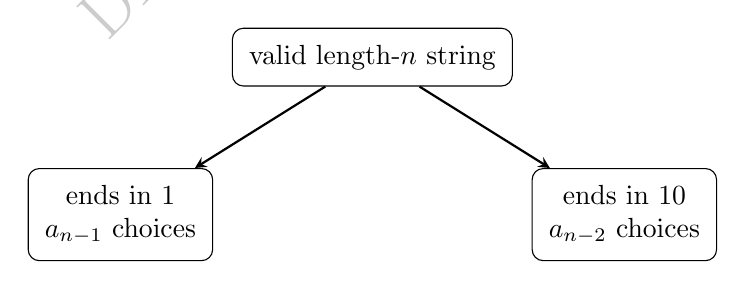
\begin{tikzpicture}[>=stealth]
    \node[draw,rounded corners,align=center,inner sep=6pt] (A) at (0,0) {valid length-$n$ string};
    \node[draw,rounded corners,align=center,inner sep=6pt] (B) at (-3.2,-2.0) {ends in $1$\\$a_{n-1}$ choices};
    \node[draw,rounded corners,align=center,inner sep=6pt] (C) at (3.2,-2.0) {ends in $10$\\$a_{n-2}$ choices};
    \draw[->,thick] (A) -- (B);
    \draw[->,thick] (A) -- (C);
\end{tikzpicture}
\end{center}

Thus $(a_n)$ satisfies the same recurrence as the Fibonacci numbers, but with different initial conditions.

\begin{examtip}[title={Standard last-symbol strategy}]
When deriving a recurrence for strings, examining the last symbol is often the cleanest approach. The key is to ensure that the resulting cases are both exhaustive and disjoint.
\end{examtip}

%==================================================
\subsection{Example: Decimal Codewords With an Even Number of Zeros}
%==================================================

A decimal string is a valid codeword if it contains an even number of zero digits. Let $a_n$ denote the number of valid codewords of length $n$.

\begin{examplebox}[title={Codeword recurrence via last digit}]
Consider a codeword of length $n$ and inspect its last digit.

\textbf{Case 1:} The last digit is nonzero.
There are $9$ choices for this digit, and the preceding $n-1$ digits must already form a valid codeword. Hence this case contributes
\[
9a_{n-1}.
\]

\textbf{Case 2:} The last digit is $0$.
Then the preceding $n-1$ digits must contain an \emph{odd} number of zeros. The total number of decimal strings of length $n-1$ is $10^{n-1}$, and among these, exactly $a_{n-1}$ have an even number of zeros. Therefore the number with an odd number of zeros is
\[
10^{n-1}-a_{n-1}.
\]
Hence this case contributes
\[
10^{n-1}-a_{n-1}.
\]

Adding the two cases gives
\[
a_n=9a_{n-1}+(10^{n-1}-a_{n-1})=8a_{n-1}+10^{n-1}.
\]
\end{examplebox}

A convenient initial condition is
\[
a_0=1,
\]
since the empty string contains $0$ zeros, which is even. Equivalently, one may use
\[
a_1=9.
\]

% Even/odd parity transition diagram for the number of 0-digits.
\begin{center}
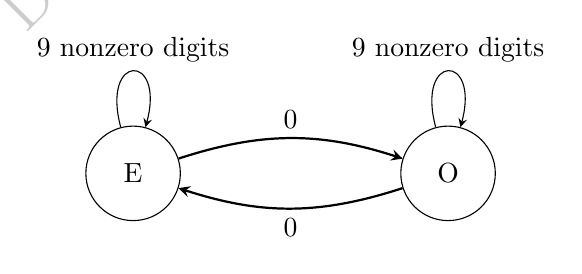
\begin{tikzpicture}[>=stealth]
    \node[draw,circle,minimum size=1.2cm] (E) at (0,0) {E};
    \node[draw,circle,minimum size=1.2cm] (O) at (4,0) {O};
    \draw[->,loop above] (E) to node[above] {$9$ nonzero digits} (E);
    \draw[->,loop above] (O) to node[above] {$9$ nonzero digits} (O);
    \draw[->,bend left=18,thick] (E) to node[above] {$0$} (O);
    \draw[->,bend left=18,thick] (O) to node[below] {$0$} (E);
\end{tikzpicture}
\end{center}

\begin{extension}[title={State augmentation viewpoint}]
This example shows that a single quantity may be insufficient unless the state captures the right information. Here the relevant hidden state is the \emph{parity} of the number of zeros. One may track even and odd states separately, then eliminate the odd state to obtain a one-variable recurrence.
\end{extension}

\begin{commonmistake}[title={Forgetting the complement count}]
In the zero-ending case, the preceding string must have an odd number of zeros, not an even number. The handout avoids introducing a second sequence by counting the odd case as
\[
10^{n-1}-a_{n-1}.
\]
\end{commonmistake}

%==================================================
\subsection{What This Handout Does Not Yet Do}
%==================================================

Handout 04 focuses on \emph{forming} recurrences and identifying initial conditions. Systematic methods for solving more general recurrence relations are deferred to Handouts 05 and 06.

\begin{examtip}[title={Scope boundary}]
In this handout, deriving the recurrence correctly is the main objective. When a closed form is not immediate, it is acceptable to stop once the recurrence and initial data have been obtained clearly.
\end{examtip}

%==================================================
\subsection{Special Techniques}
%==================================================

\subsubsection*{1. Define the state precisely}
A recurrence begins with a precise quantity. State clearly what $a_n$ counts or measures, and what the size parameter $n$ means.

\subsubsection*{2. Split by the last step or last symbol}
For process problems, inspect the final move. For strings, inspect the last symbol. This often produces natural disjoint cases.

\subsubsection*{3. Separate old contribution from new contribution}
In growth models, write the current total as
\[
\text{previous total} + \text{new amount added now}.
\]
This is the key idea in the graduate-student job problem.

\subsubsection*{4. Use complement counting when a second state is awkward}
In the codeword example, the odd-zero case is counted as
\[
10^{n-1}-a_{n-1}
\]
instead of introducing a second recurrence immediately.

\subsubsection*{5. Compare with known sequences carefully}
Two different problems may satisfy the same recurrence. Do not conclude that the sequences are identical until the initial conditions are also checked.

\subsubsection*{6. Compute a few early terms as a plausibility check}
Before trusting a recurrence, calculate the first few values manually. This helps detect missing cases or incorrect initial conditions.

\begin{extension}[title={A robust recurrence-building workflow}]
For a new problem, try the following order:
\begin{enumerate}[leftmargin=*]
    \item choose the parameter $n$;
    \item define the state variable precisely;
    \item classify size-$n$ objects into natural disjoint cases;
    \item express each case in terms of smaller sizes;
    \item write initial conditions separately;
    \item test the recurrence on small values.
\end{enumerate}
\end{extension}

%==================================================
\subsection{Summary Table}
%==================================================

\begin{center}
\small
\begin{tabular}{@{}p{0.30\textwidth}p{0.29\textwidth}p{0.29\textwidth}@{}}
\toprule
\textbf{Problem} & \textbf{State variable} & \textbf{Recurrence / data} \\
\midrule
Tower of Hanoi & $H_n$ = minimum moves for $n$ disks & $H_1=1$, \\ $H_n=2H_{n-1}+1$ \\
Compound interest & $P_n$ = amount after $n$ years & $P_0=10{,}000$, \\ $P_n=1.11P_{n-1}$ \\
Graduate-student job problem & $f_n$ = number of professors in year $n$ & $f_0=0$, $f_1=1$, \\ $f_n=f_{n-1}+f_{n-2}$ \\
No consecutive zeros & $a_n$ = valid bit strings of length $n$ & $a_1=2$, $a_2=3$, \\ $a_n=a_{n-1}+a_{n-2}$ \\
Even number of zero digits & $a_n$ = valid decimal codewords of length $n$ & $a_0=1$, \\ $a_n=8a_{n-1}+10^{n-1}$ \\
\bottomrule
\end{tabular}
\end{center}

\begin{commonmistake}[title={Final warning for Handout 04}]
A recurrence is not obtained by observing a pattern in a few numerical values alone. The recurrence must come from a mathematically justified decomposition of the problem into smaller cases.
\end{commonmistake}}{}
\IfFileExists{chapters/handout05.tex}{% Source reference: :contentReference[oaicite:0]{index=0}
\part{Recurrence Relations}
\section{Handout 05: Linear Homogeneous Recurrence Relations}

\subsection{Overview}

This handout studies how to \emph{solve} linear homogeneous recurrence relations with constant coefficients. The main ideas are:
\begin{itemize}[leftmargin=*]
    \item the definition of a linear homogeneous recurrence relation of degree $k$;
    \item uniqueness once $k$ initial conditions are specified;
    \item the characteristic equation;
    \item the solution form for degree-$2$ recurrences with distinct roots;
    \item the modified solution form for repeated roots;
    \item the extension to higher degree and, optionally, repeated multiplicities.
\end{itemize}

The main modelling principle is that a recurrence relation is converted into an algebraic equation by testing exponential trial solutions of the form
\[
a_n=r^n.
\]

\begin{examtip}[title={Main workflow for this handout}]
To solve a linear homogeneous recurrence with constant coefficients:
\begin{enumerate}[leftmargin=*]
    \item write down the characteristic equation;
    \item find its characteristic roots;
    \item write the correct general solution form from the root structure;
    \item use the initial conditions to determine the constants.
\end{enumerate}
\end{examtip}

%==================================================
\subsection{Linear Homogeneous Recurrence Relations}
%==================================================

\begin{definition}{Linear homogeneous recurrence relation}{linear-homogeneous}
A \emph{linear homogeneous recurrence relation of degree $k$ with constant coefficients} is a recurrence relation of the form
\[
a_n=c_1a_{n-1}+c_2a_{n-2}+\cdots+c_ka_{n-k},
\]
where $c_1,\dots,c_k$ are real constants and
\[
c_k\neq 0.
\]
\end{definition}

The adjectives in the definition matter:
\begin{itemize}[leftmargin=*]
    \item \emph{linear}: the terms $a_{n-1},\dots,a_{n-k}$ appear only to the first power and are not multiplied together;
    \item \emph{homogeneous}: there is no extra term independent of the sequence values;
    \item \emph{constant coefficients}: the coefficients $c_1,\dots,c_k$ do not depend on $n$.
\end{itemize}

\begin{examplebox}[title={Examples and non-examples}]
\[
f_n=f_{n-1}+f_{n-2}
\]
is linear, homogeneous, degree $2$, with constant coefficients.

\[
a_n=a_{n-1}+a_{n-2}^2
\]
is not linear.

\[
H_n=H_{n-1}+2
\]
is not homogeneous.

\[
X_n=nX_{n-1}
\]
does not have constant coefficients.
\end{examplebox}

\begin{keyformula}[title={General form}]
\[
a_n=c_1a_{n-1}+c_2a_{n-2}+\cdots+c_ka_{n-k},
\qquad c_k\neq 0.
\]
\end{keyformula}

\begin{commonmistake}[title={Checking only the shape of the left-hand side}]
A recurrence can look similar to the standard form and still fail one of the required conditions. Always check linearity, homogeneity, and constancy of coefficients separately.
\end{commonmistake}

%==================================================
\subsection{Uniqueness from Initial Conditions}
%==================================================

\begin{theorem}{Uniqueness of solutions}{uniqueness}
Suppose
\[
a_n=c_1a_{n-1}+c_2a_{n-2}+\cdots+c_ka_{n-k}
\]
is a linear homogeneous recurrence relation of degree $k$, and suppose the initial values
\[
a_0,a_1,\dots,a_{k-1}
\]
are given. Then the sequence $(a_n)$ is uniquely determined.
\end{theorem}

\begin{proof}
The recurrence gives $a_k$ in terms of $a_0,\dots,a_{k-1}$. Once $a_k$ is determined, it gives $a_{k+1}$ in terms of $a_1,\dots,a_k$, and so on. By repeated application, every later term is determined uniquely from the recurrence and the initial data.
\end{proof}

\begin{examtip}[title={Why the number of initial conditions equals the degree}]
A degree-$k$ recurrence refers back to the previous $k$ terms. Therefore one needs exactly $k$ starting values to determine the entire sequence.
\end{examtip}

%==================================================
\subsection{Characteristic Equation}
%==================================================

The central idea is to test whether the recurrence admits solutions of exponential form.

\begin{theorem}{Characteristic equation principle}{characteristic-principle}
For the recurrence
\[
a_n=c_1a_{n-1}+c_2a_{n-2}+\cdots+c_ka_{n-k},
\]
if we substitute a trial solution
\[
a_n=r^n,
\]
then $r$ must satisfy
\[
r^k-c_1r^{k-1}-c_2r^{k-2}-\cdots-c_{k-1}r-c_k=0.
\]
This polynomial equation is called the \emph{characteristic equation}.
\end{theorem}

\begin{proof}
Substituting $a_n=r^n$ into the recurrence gives
\[
r^n=c_1r^{n-1}+c_2r^{n-2}+\cdots+c_kr^{n-k}.
\]
Assuming $r\neq 0$, divide by $r^{n-k}$ to obtain
\[
r^k-c_1r^{k-1}-c_2r^{k-2}-\cdots-c_{k-1}r-c_k=0.
\]
This is the required polynomial equation.
\end{proof}

\begin{keyformula}[title={Characteristic equation}]
For
\[
a_n=c_1a_{n-1}+c_2a_{n-2}+\cdots+c_ka_{n-k},
\]
the characteristic equation is
\[
r^k-c_1r^{k-1}-c_2r^{k-2}-\cdots-c_{k-1}r-c_k=0.
\]
\end{keyformula}

\begin{examplebox}[title={Characteristic equations}]
For
\[
f_n=f_{n-1}+f_{n-2},
\]
the characteristic equation is
\[
r^2-r-1=0.
\]

For
\[
a_n=a_{n-1}+3a_{n-2}-2a_{n-3},
\]
the characteristic equation is
\[
r^3-r^2-3r+2=0.
\]
\end{examplebox}

\begin{extension}[title={Why exponential trial solutions are natural}]
A linear homogeneous recurrence with constant coefficients treats every time step in exactly the same way. Exponential sequences are the discrete analogue of eigenfunctions for such translation-invariant operators, which is why the characteristic-equation method works so cleanly.
\end{extension}

%==================================================
\subsection{Degree 2 with Distinct Roots}
%==================================================

We now focus on
\[
a_n=c_1a_{n-1}+c_2a_{n-2}.
\]
Its characteristic equation is
\[
r^2-c_1r-c_2=0.
\]

\begin{theorem}{Distinct-root case for degree 2}{distinct-root-degree-two}
Suppose the characteristic equation
\[
r^2-c_1r-c_2=0
\]
has two distinct roots $r_1$ and $r_2$. Then a sequence $(a_n)$ satisfies
\[
a_n=c_1a_{n-1}+c_2a_{n-2}
\]
if and only if
\[
a_n=h_1r_1^n+h_2r_2^n
\qquad (n=0,1,2,\dots),
\]
for some constants $h_1,h_2$.
\end{theorem}

\begin{proof}
Since $r_1$ and $r_2$ are roots of the characteristic equation,
\[
r_1^2=c_1r_1+c_2,\qquad r_2^2=c_1r_2+c_2.
\]
Hence, if
\[
a_n=h_1r_1^n+h_2r_2^n,
\]
then
\begin{align*}
c_1a_{n-1}+c_2a_{n-2}
&=c_1(h_1r_1^{n-1}+h_2r_2^{n-1})+c_2(h_1r_1^{n-2}+h_2r_2^{n-2})\\
&=h_1r_1^{n-2}(c_1r_1+c_2)+h_2r_2^{n-2}(c_1r_2+c_2)\\
&=h_1r_1^n+h_2r_2^n\\
&=a_n.
\end{align*}
This proves the ``if'' direction. The converse follows from uniqueness: the initial conditions determine unique values of $h_1,h_2$, and any solution with the same initial conditions must coincide with this form.
\end{proof}

\subsubsection{Determining the constants}

Given initial values $a_0$ and $a_1$, solve
\[
a_0=h_1+h_2,
\qquad
a_1=h_1r_1+h_2r_2.
\]
Since $r_1\neq r_2$, the constants are uniquely determined:
\[
h_1=\frac{a_1-a_0r_2}{r_1-r_2},
\qquad
h_2=\frac{a_0r_1-a_1}{r_1-r_2}.
\]

\begin{examplebox}[title={Example 3 from the handout}]
Solve
\[
a_n=a_{n-1}+2a_{n-2},
\qquad
a_0=2,\ a_1=7.
\]

The characteristic equation is
\[
r^2-r-2=0=(r-2)(r+1),
\]
so the roots are
\[
r_1=2,\qquad r_2=-1.
\]
Hence
\[
a_n=h_1\,2^n+h_2(-1)^n.
\]
Use the initial conditions:
\[
2=h_1+h_2,
\qquad
7=2h_1-h_2.
\]
Solving gives
\[
h_1=3,\qquad h_2=-1.
\]
Therefore
\[
\boxed{a_n=3\cdot 2^n-(-1)^n.}
\]
\end{examplebox}

\begin{examplebox}[title={Fibonacci sequence}]
Solve
\[
f_n=f_{n-1}+f_{n-2},
\qquad
f_0=0,\ f_1=1.
\]

The characteristic equation is
\[
r^2-r-1=0,
\]
whose roots are
\[
r_1=\frac{1+\sqrt5}{2},
\qquad
r_2=\frac{1-\sqrt5}{2}.
\]
Hence
\[
f_n=h_1r_1^n+h_2r_2^n.
\]
Using
\[
0=h_1+h_2,
\qquad
1=h_1r_1+h_2r_2,
\]
one obtains
\[
h_1=\frac{1}{\sqrt5},
\qquad
h_2=-\frac{1}{\sqrt5}.
\]
Therefore
\[
\boxed{
f_n=
\frac{1}{\sqrt5}\left(\frac{1+\sqrt5}{2}\right)^n
-
\frac{1}{\sqrt5}\left(\frac{1-\sqrt5}{2}\right)^n
}.
\]
\end{examplebox}

\begin{commonmistake}[title={Forgetting to use both initial conditions}]
For a degree-$2$ recurrence, the general solution contains two constants. Both initial conditions are needed to determine them.
\end{commonmistake}

%==================================================
\subsection{Repeated Root for Degree 2}
%==================================================

If the characteristic equation has only one root, the previous two-term form collapses and must be modified.

\begin{theorem}{Repeated-root case for degree 2}{repeated-root-degree-two}
Suppose the recurrence
\[
a_n=c_1a_{n-1}+c_2a_{n-2}
\]
has characteristic equation
\[
r^2-c_1r-c_2=0
\]
with a repeated root $r_0$. Then $(a_n)$ is a solution if and only if
\[
a_n=h_1r_0^n+h_2nr_0^n
=(h_1+h_2n)r_0^n
\qquad (n=0,1,2,\dots),
\]
for some constants $h_1,h_2$.
\end{theorem}

\begin{keyformula}[title={Repeated-root form}]
If the characteristic equation has repeated root $r_0$, then
\[
a_n=(h_1+h_2n)r_0^n.
\]
\end{keyformula}

\begin{examplebox}[title={Plant model from the handout}]
Each plant reproduces once during the first year of its life, then never again, and all plants live forever. Assume there is $1$ plant in year $1$. Let $p_n$ be the number of plants in year $n$.

From the handout,
\[
p_0=0,\qquad p_1=1,
\]
and
\[
p_n=p_{n-1}+(p_{n-1}-p_{n-2})=2p_{n-1}-p_{n-2}.
\]
The characteristic equation is
\[
r^2-2r+1=0=(r-1)^2,
\]
so the repeated root is
\[
r_0=1.
\]
Hence
\[
p_n=(h_1+h_2n)1^n=h_1+h_2n.
\]
Using
\[
p_0=0,\qquad p_1=1,
\]
we get
\[
h_1=0,\qquad h_2=1.
\]
Therefore
\[
\boxed{p_n=n.}
\]
\end{examplebox}

\begin{examplebox}[title={Example 5 from the handout}]
Solve
\[
a_n=6a_{n-1}-9a_{n-2},
\qquad
a_0=1,\ a_1=6.
\]

The characteristic equation is
\[
r^2-6r+9=0=(r-3)^2,
\]
so the repeated root is
\[
r_0=3.
\]
Hence
\[
a_n=(h_1+h_2n)3^n.
\]
Use the initial conditions:
\[
1=a_0=h_1,
\]
and
\[
6=a_1=(h_1+h_2)3=(1+h_2)3.
\]
Thus
\[
h_2=1.
\]
Therefore
\[
\boxed{a_n=(n+1)3^n.}
\]
\end{examplebox}

\begin{extension}[title={Why the extra factor of $n$ appears}]
When a root is repeated, the two naive solutions $r_0^n$ and $r_0^n$ are linearly dependent, so they do not provide enough freedom to satisfy arbitrary initial conditions. The extra factor $n$ creates a second independent solution.
\end{extension}

%==================================================
\subsection{Higher Degree with Distinct Roots}
%==================================================

The degree-$2$ picture extends directly to higher degree.

\begin{theorem}{Degree $k$ with distinct roots}{degree-k-distinct}
Consider
\[
a_n=c_1a_{n-1}+c_2a_{n-2}+\cdots+c_ka_{n-k},
\]
and suppose its characteristic equation
\[
r^k-c_1r^{k-1}-c_2r^{k-2}-\cdots-c_{k-1}r-c_k=0
\]
has $k$ distinct roots
\[
r_1,r_2,\dots,r_k.
\]
Then the general solution is
\[
a_n=h_1r_1^n+h_2r_2^n+\cdots+h_kr_k^n,
\]
where the constants $h_1,\dots,h_k$ are determined by the $k$ initial conditions.
\end{theorem}

\begin{examplebox}[title={Example 6 from the handout}]
Solve
\[
a_n=6a_{n-1}-11a_{n-2}+6a_{n-3},
\qquad
a_0=2,\ a_1=5,\ a_2=15.
\]

The characteristic equation is
\[
r^3-6r^2+11r-6=0.
\]
It factors as
\[
(r-1)(r-2)(r-3)=0,
\]
so the roots are
\[
1,\ 2,\ 3.
\]
Hence
\[
a_n=h_1\cdot 1^n+h_2\cdot 2^n+h_3\cdot 3^n.
\]
Use the initial conditions:
\[
2=h_1+h_2+h_3,
\]
\[
5=h_1+2h_2+3h_3,
\]
\[
15=h_1+4h_2+9h_3.
\]
Solving gives
\[
h_1=1,\qquad h_2=-1,\qquad h_3=2.
\]
Therefore
\[
\boxed{a_n=1-2^n+2\cdot 3^n.}
\]
\end{examplebox}

\begin{examtip}[title={Higher-degree structure}]
For degree $k$, the number of arbitrary constants in the solution must match the number of initial conditions. Distinct characteristic roots supply exactly one independent exponential term each.
\end{examtip}

%==================================================
\subsection{Multiplicity (Optional)}
%==================================================

\begin{definition}{Multiplicity of a root}{multiplicity-def}
Suppose the characteristic polynomial factors as
\[
(r-r_1)^{m_1}(r-r_2)^{m_2}\cdots(r-r_t)^{m_t},
\]
where $r_1,\dots,r_t$ are distinct and
\[
m_1+m_2+\cdots+m_t=k.
\]
Then $r_i$ is said to be a root of multiplicity $m_i$.
\end{definition}

\begin{theorem}{General multiplicity form (optional)}{multiplicity-theorem}
If the characteristic equation of a degree-$k$ linear homogeneous recurrence has distinct roots
\[
r_1,\dots,r_t
\]
with multiplicities
\[
m_1,\dots,m_t,
\]
then the general solution is
\[
a_n=
(h_{1,0}+h_{1,1}n+\cdots+h_{1,m_1-1}n^{m_1-1})r_1^n
+\cdots+
(h_{t,0}+h_{t,1}n+\cdots+h_{t,m_t-1}n^{m_t-1})r_t^n.
\]
\end{theorem}

\begin{examplebox}[title={Optional repeated-root example}]
Solve
\[
a_n=-3a_{n-1}-3a_{n-2}-a_{n-3},
\qquad
a_0=1,\ a_1=-2,\ a_2=-1.
\]

The characteristic equation is
\[
r^3+3r^2+3r+1=0=(r+1)^3.
\]
So the root $-1$ has multiplicity $3$. Hence
\[
a_n=(h_{1,0}+h_{1,1}n+h_{1,2}n^2)(-1)^n.
\]
Using the given initial conditions, one finds
\[
h_{1,0}=1,\qquad h_{1,1}=3,\qquad h_{1,2}=-2.
\]
Therefore
\[
\boxed{a_n=(1+3n-2n^2)(-1)^n.}
\]
\end{examplebox}

\begin{extension}[title={Repeated roots produce polynomial factors}]
Multiplicity $m$ of a root $r$ produces the family
\[
r^n,\ nr^n,\ n^2r^n,\ \dots,\ n^{m-1}r^n.
\]
These are the discrete recurrence analogues of repeated-root solution forms in linear differential equations.
\end{extension}

%==================================================
\subsection{Simultaneous Recurrence Relations}
%==================================================

The handout also introduces systems such as
\[
a_n=a_{n-1}+b_{n-1},
\qquad
b_n=a_{n-1}-b_{n-1},
\]
with
\[
a_0=1,\qquad b_0=2.
\]

A standard approach is to eliminate one variable.

\begin{examplebox}[title={Eliminating one variable in a system}]
From
\[
a_n=a_{n-1}+b_{n-1},
\qquad
b_n=a_{n-1}-b_{n-1},
\]
we obtain
\[
a_{n+1}=a_n+b_n.
\]
But
\[
b_n=a_{n-1}-b_{n-1}=a_{n-1}-(a_n-a_{n-1})=2a_{n-1}-a_n.
\]
Hence
\[
a_{n+1}=a_n+(2a_{n-1}-a_n)=2a_{n-1}.
\]
So $a_n$ satisfies the second-order recurrence
\[
a_{n+1}=2a_{n-1}.
\]
Using
\[
a_0=1,\qquad a_1=a_0+b_0=3,
\]
one can continue or solve this reduced recurrence directly. Once $(a_n)$ is known, recover $(b_n)$ from
\[
b_n=a_n-a_{n-1}.
\]
\end{examplebox}

\begin{examtip}[title={System strategy}]
For simultaneous recurrences, try to reduce the system to one recurrence in one variable by substitution or elimination. After that, solve the reduced recurrence using the characteristic equation.
\end{examtip}

%==================================================
\subsection{Special Techniques}
%==================================================

\subsubsection*{1. Trial solution \(a_n=r^n\)}
For linear homogeneous recurrences with constant coefficients, this is the standard gateway to the characteristic equation.

\subsubsection*{2. Distinguish root structure first}
Before using initial conditions, decide whether the characteristic polynomial has:
\begin{itemize}[leftmargin=*]
    \item distinct roots,
    \item repeated roots,
    \item or several roots with multiplicities.
\end{itemize}

\subsubsection*{3. Match the number of constants to the degree}
A degree-$k$ recurrence requires $k$ arbitrary constants in the general solution form.

\subsubsection*{4. Solve the linear system cleanly}
After finding the general form, substitute the initial conditions immediately and solve for the constants in an organized way.

\subsubsection*{5. Eliminate variables in simultaneous systems}
When two sequences are coupled, try to derive a single recurrence for one of them first.

\subsubsection*{6. Check small values}
After finding a closed form, verify the first few terms against the recurrence and the initial data.

\begin{commonmistake}[title={Using the wrong repeated-root form}]
If the characteristic polynomial has a repeated root, the form
\[
h_1r^n+h_2r^n
\]
is not correct, because the two terms are the same. The correct second independent term is
\[
nr^n.
\]
\end{commonmistake}

%==================================================
\subsection{Summary Table}
%==================================================

\begin{center}
\scriptsize
\begin{tabular}{@{}p{0.33\textwidth}p{0.28\textwidth}p{0.28\textwidth}@{}}
\toprule
\textbf{Recurrence type} & \textbf{Characteristic data} & \textbf{General solution form} \\
\midrule
Degree $2$ & distinct roots $r_1,r_2$ &
\[
a_n=h_1r_1^n+h_2r_2^n
\]
\\[1.0em]
Degree $2$ & repeated root $r_0$ &
\[
a_n=(h_1+h_2n)r_0^n
\]
\\[1.0em]
Degree $k$ & distinct roots $r_1,\dots,r_k$ &
\[
a_n=h_1r_1^n+\cdots+h_kr_k^n
\]
\\[1.0em]
Degree $k$ & root $r_i$ of multiplicity $m_i$ &
\[
(\text{polynomial in }n\text{ of degree }m_i-1)r_i^n
\]
\\
\bottomrule
\end{tabular}
\end{center}

\begin{examtip}[title={Final checklist for Handout 05}]
Before finalizing a solution, confirm:
\begin{enumerate}[leftmargin=*]
    \item the recurrence is linear, homogeneous, and has constant coefficients;
    \item the characteristic equation is written correctly;
    \item the root structure has been identified correctly;
    \item the general solution form matches that root structure;
    \item the initial conditions have been used to determine all constants.
\end{enumerate}
\end{examtip}
}{}
\IfFileExists{chapters/handout06.tex}{\part{Recurrence Relations}
\section{Handout 06: Linear Non-Homogeneous Recurrence Relations}

\subsection{Overview}

This handout completes Part~II on recurrence relations. We now study \emph{linear non-homogeneous recurrence relations with constant coefficients}. The main point is that such a recurrence is solved in two steps:
\begin{enumerate}[leftmargin=*]
    \item solve the associated homogeneous recurrence;
    \item find one particular solution of the non-homogeneous recurrence.
\end{enumerate}

The general solution is then obtained by adding these two pieces.

The main topics are:
\begin{itemize}[leftmargin=*]
    \item definition of a linear non-homogeneous recurrence relation;
    \item associated homogeneous recurrence;
    \item the structure theorem
    \[
    a_n=a_n^{(p)}+b_n;
    \]
    \item method of undetermined coefficients for polynomial forcing terms;
    \item method of undetermined coefficients for exponential forcing terms;
    \item how to modify the trial form when resonance occurs.
\end{itemize}

\begin{examtip}[title={Main workflow for Handout 06}]
To solve
\[
a_n=c_1a_{n-1}+c_2a_{n-2}+\cdots+c_ka_{n-k}+F(n),
\]
use the following order:
\begin{enumerate}[leftmargin=*]
    \item solve the associated homogeneous recurrence;
    \item guess a suitable particular solution \(a_n^{(p)}\);
    \item substitute to determine the unknown coefficients;
    \item add the homogeneous part;
    \item impose the initial conditions.
\end{enumerate}
\end{examtip}

%==================================================
\subsection{Linear Non-Homogeneous Recurrence Relations}
%==================================================

\begin{definition}{Linear non-homogeneous recurrence relation}{nonhomogeneous-def}
A \emph{linear non-homogeneous recurrence relation of degree \(k\) with constant coefficients} is a recurrence of the form
\[
a_n=c_1a_{n-1}+c_2a_{n-2}+\cdots+c_ka_{n-k}+F(n),
\]
where \(c_1,\dots,c_k\) are real constants, \(c_k\neq 0\), and \(F(n)\neq 0\) depends only on \(n\).
\end{definition}

\begin{definition}{Associated homogeneous recurrence}{associated-homogeneous}
The \emph{associated homogeneous recurrence relation} of
\[
a_n=c_1a_{n-1}+c_2a_{n-2}+\cdots+c_ka_{n-k}+F(n)
\]
is obtained by removing the forcing term \(F(n)\):
\[
b_n=c_1b_{n-1}+c_2b_{n-2}+\cdots+c_kb_{n-k}.
\]
\end{definition}

\begin{examplebox}[title={Examples}]
\[
f_n=f_{n-1}+f_{n-2}+3
\]
has associated homogeneous recurrence
\[
b_n=b_{n-1}+b_{n-2}.
\]

\[
a_n=3a_{n-1}+5a_{n-2}+n^2
\]
has associated homogeneous recurrence
\[
b_n=3b_{n-1}+5b_{n-2}.
\]

\[
a_n=2a_{n-1}-5a_{n-3}-2^n+n^2-5
\]
has associated homogeneous recurrence
\[
b_n=2b_{n-1}-5b_{n-3}.
\]
\end{examplebox}

\begin{commonmistake}[title={Adding two non-homogeneous solutions}]
If \((a_n)\) and \((d_n)\) are both solutions of the same non-homogeneous recurrence
\[
x_n=c_1x_{n-1}+\cdots+c_kx_{n-k}+F(n),
\]
then \((a_n+d_n)\) is \emph{not} generally a solution, because the forcing term becomes
\[
2F(n).
\]
This differs from the homogeneous case.
\end{commonmistake}

\begin{extension}[title={What survives from the homogeneous theory}]
The homogeneous solutions still form a vector space. The non-homogeneous solutions do not. Instead, the set of non-homogeneous solutions is a translate of the homogeneous solution space by any one particular solution.
\end{extension}

%==================================================
\subsection{Structure Theorem}
%==================================================

\begin{theorem}{General form of all solutions}{structure-theorem}
Consider
\[
a_n=c_1a_{n-1}+c_2a_{n-2}+\cdots+c_ka_{n-k}+F(n).
\]
If \(\bigl(a_n^{(p)}\bigr)\) is one particular solution of this recurrence, then every solution is of the form
\[
a_n=a_n^{(p)}+b_n,
\]
where \((b_n)\) is a solution of the associated homogeneous recurrence
\[
b_n=c_1b_{n-1}+c_2b_{n-2}+\cdots+c_kb_{n-k}.
\]
\end{theorem}

\begin{proof}
Let \((d_n)\) be any solution of the non-homogeneous recurrence. Then
\[
d_n=c_1d_{n-1}+c_2d_{n-2}+\cdots+c_kd_{n-k}+F(n),
\]
while the particular solution satisfies
\[
a_n^{(p)}=c_1a_{n-1}^{(p)}+c_2a_{n-2}^{(p)}+\cdots+c_ka_{n-k}^{(p)}+F(n).
\]
Subtracting gives
\[
d_n-a_n^{(p)}
=
c_1(d_{n-1}-a_{n-1}^{(p)})
+\cdots+
c_k(d_{n-k}-a_{n-k}^{(p)}).
\]
Hence the sequence
\[
b_n=d_n-a_n^{(p)}
\]
satisfies the associated homogeneous recurrence. Therefore
\[
d_n=a_n^{(p)}+b_n.
\]
Conversely, if \(b_n\) satisfies the associated homogeneous recurrence, then \(a_n^{(p)}+b_n\) satisfies the original non-homogeneous recurrence by direct substitution.
\end{proof}

\begin{keyformula}[title={General solution of a linear non-homogeneous recurrence}]
\[
\boxed{
\text{general solution}
=
\text{particular solution}
+
\text{general homogeneous solution}.
}
\]
\end{keyformula}

% Schematic decomposition of a non-homogeneous solution.
\begin{center}
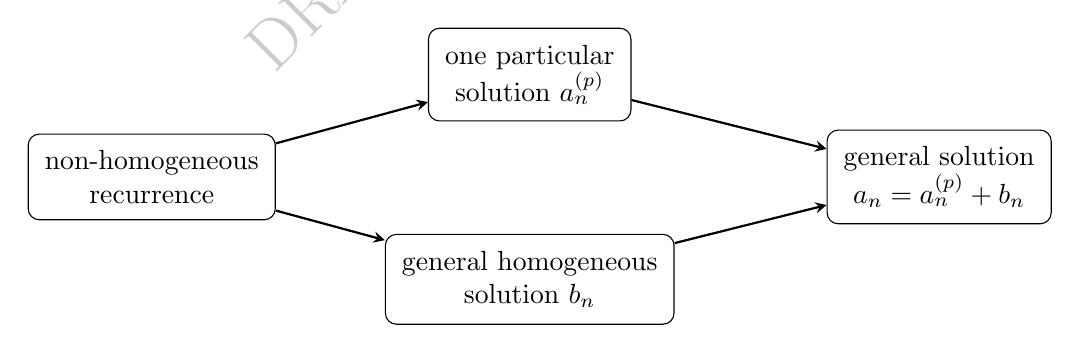
\begin{tikzpicture}[>=stealth]
    \node[draw,rounded corners,align=center,inner sep=6pt] (A) at (0,0) {non-homogeneous\\recurrence};
    \node[draw,rounded corners,align=center,inner sep=6pt] (B) at (4.8,1.3) {one particular\\solution \(a_n^{(p)}\)};
    \node[draw,rounded corners,align=center,inner sep=6pt] (C) at (4.8,-1.3) {general homogeneous\\solution \(b_n\)};
    \node[draw,rounded corners,align=center,inner sep=6pt] (D) at (10.0,0) {general solution\\\(a_n=a_n^{(p)}+b_n\)};
    \draw[->,thick] (A) -- (B);
    \draw[->,thick] (A) -- (C);
    \draw[->,thick] (B) -- (D);
    \draw[->,thick] (C) -- (D);
\end{tikzpicture}
\end{center}

\begin{examtip}[title={Why this theorem matters}]
One never needs to find \emph{all} non-homogeneous solutions directly. It is enough to find:
\begin{itemize}[leftmargin=*]
    \item one particular solution;
    \item the full homogeneous solution.
\end{itemize}
\end{examtip}

%==================================================
\subsection{A First Worked Example: Polynomial Forcing}
%==================================================

\begin{examplebox}[title={Example 10 from the handout}]
Find the solution of
\[
a_n=3a_{n-1}+2n,
\qquad a_1=3.
\]

\textbf{Step 1: Solve the associated homogeneous recurrence.}
The associated homogeneous recurrence is
\[
b_n=3b_{n-1},
\]
whose general solution is
\[
b_n=h\cdot 3^n,
\]
where \(h\) is a constant.

\textbf{Step 2: Find a particular solution.}
Here the forcing term
\[
F(n)=2n
\]
is a polynomial of degree \(1\). Since \(1\) is not a root of the homogeneous characteristic equation
\[
r-3=0,
\]
try a linear particular solution
\[
a_n^{(p)}=cn+d.
\]
Substitute:
\[
cn+d=3(c(n-1)+d)+2n.
\]
Expand:
\[
cn+d=3cn-3c+3d+2n.
\]
Move everything to one side:
\[
(2+2c)n+(2d-3c)=0.
\]
Hence
\[
2+2c=0,\qquad 2d-3c=0.
\]
So
\[
c=-1,\qquad d=-\frac32.
\]
Thus
\[
a_n^{(p)}=-n-\frac32.
\]

\textbf{Step 3: Form the general solution.}
By the structure theorem,
\[
a_n=a_n^{(p)}+b_n
=
-n-\frac32+h\cdot 3^n.
\]

\textbf{Step 4: Use the initial condition.}
Since \(a_1=3\),
\[
3=-1-\frac32+3h,
\]
so
\[
3h=\frac{11}{2}
\qquad\Longrightarrow\qquad
h=\frac{11}{6}.
\]
Therefore
\[
\boxed{
a_n=-n-\frac32+\frac{11}{6}\,3^n.
}
\]
\end{examplebox}

\begin{examplebox}[title={Second polynomial example from the handout}]
Find the solution of
\[
a_n=-2a_{n-1}+n+1,
\qquad a_0=2.
\]

The associated homogeneous recurrence is
\[
b_n=-2b_{n-1},
\]
so
\[
b_n=h(-2)^n.
\]

Since \(F(n)=n+1\) is a polynomial of degree \(1\), and \(1\) is not a root of the characteristic equation
\[
r+2=0,
\]
try
\[
a_n^{(p)}=cn+d.
\]
Substitute:
\[
cn+d=-2(c(n-1)+d)+n+1.
\]
Expand:
\[
cn+d=-2cn+2c-2d+n+1.
\]
Rearranging gives
\[
(1-3c)n+(1+2c-3d)=0.
\]
Hence
\[
1-3c=0,\qquad 1+2c-3d=0.
\]
So
\[
c=\frac13,\qquad d=\frac59.
\]
Thus
\[
a_n^{(p)}=\frac{n}{3}+\frac59.
\]
Hence the general solution is
\[
a_n=\frac{n}{3}+\frac59+h(-2)^n.
\]
Using \(a_0=2\),
\[
2=\frac59+h,
\]
so
\[
h=\frac{13}{9}.
\]
Therefore
\[
\boxed{
a_n=\frac{n}{3}+\frac59+\frac{13}{9}(-2)^n.
}
\]
\end{examplebox}

%==================================================
\subsection{Polynomial Forcing Terms}
%==================================================

The handout gives a standard guessing rule when \(F(n)\) is a polynomial.

\begin{theorem}{Trial form for polynomial forcing}{poly-trial}
Suppose
\[
a_n=c_1a_{n-1}+c_2a_{n-2}+\cdots+c_ka_{n-k}+F(n),
\]
where
\[
F(n)=b_tn^t+b_{t-1}n^{t-1}+\cdots+b_1n+b_0
\]
is a polynomial of degree \(t\).

\begin{enumerate}[leftmargin=*]
    \item If \(1\) is \emph{not} a root of the characteristic equation of the associated homogeneous recurrence, try
    \[
    a_n^{(p)}=p_tn^t+p_{t-1}n^{t-1}+\cdots+p_1n+p_0.
    \]
    \item If \(1\) \emph{is} a root of the characteristic equation, try
    \[
    a_n^{(p)}=n\bigl(p_tn^t+p_{t-1}n^{t-1}+\cdots+p_1n+p_0\bigr).
    \]
\end{enumerate}
\end{theorem}

\begin{keyformula}[title={Polynomial forcing rule}]
If \(F(n)\) is polynomial of degree \(t\), then:
\[
\text{try degree }t
\quad\text{or}\quad
n\times\text{degree }t
\]
according to whether \(1\) is not a root or is a root of the characteristic equation.
\end{keyformula}

\begin{examplebox}[title={Handout question: what should we try?}]
Suppose
\[
a_n=a_{n-1}+n.
\]
What trial form should be used?

The associated homogeneous recurrence is
\[
b_n=b_{n-1},
\]
whose characteristic equation is
\[
r-1=0.
\]
Thus \(1\) is a root. Since the forcing term \(n\) is a polynomial of degree \(1\), the correct trial is
\[
a_n^{(p)}=n(cn+d)=cn^2+dn.
\]
\end{examplebox}

\begin{commonmistake}[title={Forgetting the extra factor \(n\)}]
If \(1\) is a root of the characteristic equation, then a plain polynomial trial overlaps with the homogeneous solution and fails. One must multiply by \(n\).

\end{commonmistake}

\begin{extension}[title={Resonance viewpoint for polynomial forcing}]
The special role of \(1\) comes from the fact that polynomial sequences are built from powers of \(n\), while the homogeneous solution corresponding to root \(1\) contains constant-type behaviour. Multiplying by \(n\) shifts the trial form out of the homogeneous solution space.
\end{extension}

%==================================================
\subsection{Exponential Forcing Terms}
%==================================================

We now consider forcing terms of the form
\[
F(n)=s^n.
\]

\begin{theorem}{Trial form for exponential forcing}{exp-trial}
Suppose
\[
a_n=c_1a_{n-1}+c_2a_{n-2}+\cdots+c_ka_{n-k}+s^n.
\]

\begin{enumerate}[leftmargin=*]
    \item If \(s\) is \emph{not} a root of the characteristic equation of the associated homogeneous recurrence, try
    \[
    a_n^{(p)}=c\,s^n.
    \]
    \item If \(s\) \emph{is} a root of the characteristic equation, try
    \[
    a_n^{(p)}=c\,n\,s^n.
    \]
\end{enumerate}
\end{theorem}

\begin{keyformula}[title={Exponential forcing rule}]
For \(F(n)=s^n\), try
\[
c\,s^n
\quad\text{or}\quad
c\,n\,s^n
\]
according to whether \(s\) is not a root or is a root of the homogeneous characteristic equation.
\end{keyformula}
\begin{examplebox}[title={Example 11 from the handout}]
Find all solutions of
\[
a_n=5a_{n-1}-6a_{n-2}+7^n.
\]

\textbf{Step 1: Solve the associated homogeneous recurrence.}
The associated homogeneous recurrence is
\[
b_n=5b_{n-1}-6b_{n-2}.
\]
Its characteristic equation is
\[
r^2-5r+6=0=(r-2)(r-3),
\]
so
\[
b_n=h_1\,2^n+h_2\,3^n.
\]

\textbf{Step 2: Find a particular solution.}
Since the forcing term is \(7^n\), and \(7\) is not a root of the characteristic equation, try
\[
a_n^{(p)}=c\,7^n.
\]
Substitute:
\[
c7^n=5c7^{n-1}-6c7^{n-2}+7^n.
\]
Multiply through by \(7^{-(n-2)}\):
\[
49c=35c-6c+49.
\]
Hence
\[
20c=49
\qquad\Longrightarrow\qquad
c=\frac{49}{20}.
\]
Thus
\[
a_n^{(p)}=\frac{49}{20}7^n.
\]

\textbf{Step 3: Combine.}
Therefore all solutions are
\[
\boxed{
a_n=\frac{49}{20}7^n+h_1\,2^n+h_2\,3^n.
}
\]
\end{examplebox}

\begin{examplebox}[title={Handout question: what should we try?}]
Suppose
\[
a_n=5a_{n-1}+5^n.
\]
What should be tried for a particular solution?

The associated homogeneous recurrence is
\[
b_n=5b_{n-1},
\]
whose characteristic equation is
\[
r-5=0.
\]
Thus \(5\) is a root. Therefore the correct trial is
\[
a_n^{(p)}=c\,n\,5^n.
\]
\end{examplebox}

\begin{commonmistake}[title={Using \(c\,s^n\) when \(s\) is already a homogeneous root}]
If \(s\) is a root of the characteristic equation, then \(s^n\) is already part of the homogeneous solution. A trial of the form \(c\,s^n\) cannot produce a genuinely new particular solution. Multiply by \(n\).
\end{commonmistake}

%==================================================
\subsection{How Initial Conditions Enter}
%==================================================

After a particular solution and the homogeneous solution have been combined, one obtains a general expression with arbitrary constants. These are determined exactly as in the homogeneous case by substituting the given initial conditions.

\begin{examplebox}[title={Tutorial 6, Question 4(a)}]
Find all solutions of
\[
a_n=2a_{n-1}+2n^2
\qquad (n\ge 2),
\]
and then determine the solution with \(a_1=4\).

The associated homogeneous recurrence is
\[
b_n=2b_{n-1},
\]
so
\[
b_n=h\,2^n.
\]

Since \(F(n)=2n^2\) is a polynomial of degree \(2\), and \(1\) is not a root of \(r-2=0\), try
\[
a_n^{(p)}=cn^2+dn+e.
\]
Substituting into
\[
a_n=2a_{n-1}+2n^2
\]
gives
\[
c=-2,\qquad d=-8,\qquad e=-12.
\]
Hence
\[
a_n^{(p)}=-2n^2-8n-12.
\]
So all solutions are
\[
a_n=h\,2^n-2n^2-8n-12.
\]
Using \(a_1=4\),
\[
4=2h-22,
\]
hence
\[
h=13.
\]
Therefore
\[
\boxed{
a_n=13\cdot 2^n-2n^2-8n-12.
}
\]
\end{examplebox}

\begin{examplebox}[title={Tutorial 6, Question 5(b)}]
Find all solutions of
\[
a_n=4a_{n-1}-3a_{n-2}+3^n.
\]

The associated homogeneous recurrence is
\[
b_n=4b_{n-1}-3b_{n-2},
\]
whose characteristic equation is
\[
r^2-4r+3=0=(r-1)(r-3).
\]
So
\[
b_n=h_1+h_2\,3^n.
\]

Since the forcing term is \(3^n\), and \(3\) is a root of the characteristic equation, try
\[
a_n^{(p)}=c\,n\,3^n.
\]
Substitute:
\[
cn3^n=4c(n-1)3^{n-1}-3c(n-2)3^{n-2}+3^n.
\]
Dividing by \(3^{n-2}\) gives
\[
9cn=12c(n-1)-3c(n-2)+9.
\]
Simplifying,
\[
9cn=9cn-6c+9,
\]
so
\[
6c=9
\qquad\Longrightarrow\qquad
c=\frac32.
\]
Therefore
\[
a_n^{(p)}=\frac32\,n\,3^n.
\]
Hence all solutions are
\[
\boxed{
a_n=h_1+h_2\,3^n+\frac32\,n\,3^n.
}
\]
\end{examplebox}

%==================================================
\subsection{Special Techniques}
%==================================================

\subsubsection*{1. Separate the problem into homogeneous part + particular part}
Always identify the associated homogeneous recurrence first. The final solution is built by adding a particular solution.

\subsubsection*{2. Diagnose the forcing term before guessing}
Check whether \(F(n)\) is polynomial, exponential, or a sum of simpler terms. The trial form should reflect the shape of the forcing term.

\subsubsection*{3. Test for resonance}
If the obvious trial overlaps with the homogeneous solution, multiply by \(n\). In this handout:
\begin{itemize}[leftmargin=*]
\item polynomial forcing is sensitive to whether \(1\) is a root;
\item exponential forcing \(s^n\) is sensitive to whether \(s\) is a root.
\end{itemize}

\subsubsection*{4. Use linearity of forcing when appropriate}
If the forcing term splits as
\[
F(n)=F_1(n)+F_2(n),
\]
and one can find particular solutions for each component separately, then their sum is a particular solution for the full recurrence.

\subsubsection*{5. Expand only as much as needed}
When comparing coefficients, collect powers of \(n\) carefully and equate coefficients systematically.

\subsubsection*{6. Keep the constants for the very end}
Do not impose initial conditions until after the full general solution
\[
a_n=a_n^{(p)}+b_n
\]
has been formed.

\begin{extension}[title={Why the method works so efficiently}]
The method of undetermined coefficients succeeds because the recurrence operator sends polynomial and exponential trial families into the same kind of families. This makes the unknown coefficients solvable by finite algebra rather than by guesswork.
\end{extension}

%==================================================
\subsection{Summary Table}
%==================================================

\begin{center}
\small
\begin{tabular}{@{}p{0.30\textwidth}p{0.28\textwidth}p{0.29\textwidth}@{}}
\toprule
\textbf{Forcing term \(F(n)\)} & \textbf{Condition} & \textbf{Trial for \(a_n^{(p)}\)} \\
\midrule
Polynomial of degree \(t\) & \(1\) not a root & degree-\(t\) polynomial \\
Polynomial of degree \(t\) & \(1\) is a root & \(n\times\) degree-\(t\) polynomial \\
Exponential \(s^n\) & \(s\) not a root & \(c\,s^n\) \\
Exponential \(s^n\) & \(s\) is a root & \(c\,n\,s^n\) \\
General case & one particular solution known & \(a_n=a_n^{(p)}+b_n\) \\
\bottomrule
\end{tabular}
\end{center}

\begin{examtip}[title={Final checklist for Handout 06}]
Before finalizing a solution, check:
\begin{enumerate}[leftmargin=*]
    \item Have I written the associated homogeneous recurrence correctly?
    \item Have I chosen a trial form that matches the forcing term?
    \item Have I checked whether an extra factor of \(n\) is needed?
    \item Have I found one particular solution correctly?
    \item Have I added the general homogeneous solution?
    \item Have I used the initial conditions only at the final stage?
\end{enumerate}
\end{examtip}

\begin{commonmistake}[title={Solving only the homogeneous part}]
A homogeneous solution alone is not a solution to the non-homogeneous recurrence unless the forcing term vanishes. One must always include a particular solution.
\end{commonmistake}}{}
\IfFileExists{chapters/handout07.tex}{% Source reference: :contentReference[oaicite:0]{index=0}
\part{Graph Theory}
\section{Handout 07: Graph Theory (1)}

\subsection{Overview}

This handout begins Part~III of the course. The emphasis is foundational: we introduce the language of graphs, basic graph invariants, and the notion of graph isomorphism. The main topics are:
\begin{itemize}[leftmargin=*]
    \item graph models and formal graph definitions;
    \item vertices, edges, adjacency, incidence, and degree;
    \item simple graphs, multigraphs, complete graphs, and cycle graphs;
    \item subgraphs and induced subgraphs;
    \item graph isomorphism and graph invariants;
    \item the Handshaking Lemma and its first consequences.
\end{itemize}

The guiding principle is that a graph is an abstract structure encoding \emph{objects} together with \emph{relationships} between them.

\begin{examtip}[title={Main mindset for Handout 07}]
A graph drawing is only a picture of an abstract object. The location of the vertices on the page, the length of edges, and whether edges are curved or straight are usually irrelevant. What matters is which vertices are connected to which.
\end{examtip}

%==================================================
\subsection{Graph Models}
%==================================================

Many real-world systems naturally lead to graphs:
\begin{itemize}[leftmargin=*]
    \item in an MRT map, stations are vertices and track connections are edges;
    \item in a friendship network, people are vertices and friendships are edges;
    \item in a molecule, atoms are vertices and chemical bonds are edges;
    \item in a flowchart, states or actions are vertices and transitions are directed edges;
    \item in the Bridges of Königsberg problem, land masses may be treated as vertices and bridges as edges.
\end{itemize}

\begin{examplebox}[title={Why these examples belong to one framework}]
In each case there is:
\begin{enumerate}[leftmargin=*]
    \item a collection of objects; and
    \item a specification of which pairs of objects are related.
\end{enumerate}
This is precisely what a graph records.
\end{examplebox}

\begin{extension}[title={Abstraction step in graph theory}]
Graph theory becomes powerful only after irrelevant geometric information is discarded. For example, an MRT map and a completely redrawn version of the same network represent the same graph if the adjacency structure is unchanged.
\end{extension}

%==================================================
\subsection{Undirected and Directed Graphs}
%==================================================

\begin{definition}{Undirected graph}{undirected-graph}
An \emph{undirected graph} is an ordered pair
\[
G=(V,E),
\]
where:
\begin{itemize}[leftmargin=*]
    \item \(V\) is a nonempty set of vertices; and
    \item \(E\) is a set of edges, where each edge has one or two endpoints in \(V\).
\end{itemize}
In a simple undirected graph, each edge is an unordered pair \(\{u,v\}\) of distinct vertices.
\end{definition}

\begin{definition}{Directed graph}{directed-graph}
A \emph{directed graph} (or \emph{digraph}) is an ordered pair
\[
G=(V,E),
\]
where \(V\) is a nonempty set of vertices and each edge in \(E\) is an ordered pair \((u,v)\), called a directed edge from \(u\) to \(v\).
\end{definition}

% Comparison of undirected and directed edges between labelled vertices.
\begin{center}
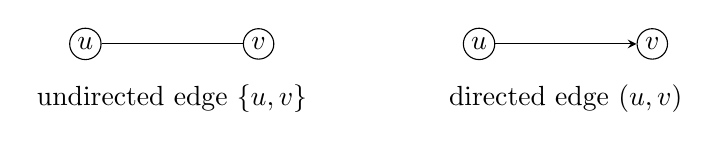
\begin{tikzpicture}[>=stealth,scale=1]
    \node[circle,draw,inner sep=1.5pt] (u1) at (0,0) {$u$};
    \node[circle,draw,inner sep=1.5pt] (v1) at (2.2,0) {$v$};
    \draw[-] (u1) -- (v1);
    \node at (1.1,-0.7) {undirected edge $\{u,v\}$};

    \node[circle,draw,inner sep=1.5pt] (u2) at (5,0) {$u$};
    \node[circle,draw,inner sep=1.5pt] (v2) at (7.2,0) {$v$};
    \draw[->] (u2) -- (v2);
    \node at (6.1,-0.7) {directed edge $(u,v)$};
\end{tikzpicture}
\end{center}

\begin{commonmistake}[title={Ordered pair versus unordered pair}]
In an undirected graph,
\[
\{u,v\}=\{v,u\},
\]
but in a digraph,
\[
(u,v)\neq (v,u)
\]
in general. The notation determines the meaning.
\end{commonmistake}

%==================================================
\subsection{Simple Graphs and Multigraphs}
%==================================================

\begin{definition}{Simple graph}{simple-graph}
An undirected graph is called \emph{simple} if:
\begin{itemize}[leftmargin=*]
    \item no self-loop \(\{v,v\}\) is allowed;
    \item there is at most one edge between any two distinct vertices.
\end{itemize}
\end{definition}

\begin{definition}{Multigraph}{multigraph}
A \emph{multigraph} is a graph in which self-loops and/or multiple edges between the same pair of vertices are allowed.
\end{definition}

If \(G=(V,E)\) is a simple graph and
\[
n=|V|,\qquad m=|E|,
\]
then every edge is determined by a choice of two distinct vertices, so
\[
0\le m\le \binom{n}{2}.
\]

\begin{keyformula}[title={Edge bound for a simple graph}]
If \(G\) is a simple graph with \(n\) vertices, then
\[
0\le |E|\le \binom{n}{2}.
\]
The upper bound is attained exactly by the complete graph \(K_n\).
\end{keyformula}

\begin{examtip}[title={Default convention in MH1301}]
Unless stated otherwise, graphs in the lectures, tutorials, and exams are assumed to be \emph{simple} graphs.
\end{examtip}

%==================================================
\subsection{Adjacency, Incidence, and Endpoints}
%==================================================

\begin{definition}{Adjacency and incidence}{adjacency-incidence}
Let \(G=(V,E)\) be an undirected graph.
\begin{itemize}[leftmargin=*]
    \item Two vertices \(u,v\in V\) are \emph{adjacent} (or \emph{neighbors}) if \(\{u,v\}\in E\).
    \item If \(e=\{u,v\}\in E\), then \(e\) is \emph{incident} with \(u\) and \(v\).
    \item The vertices \(u\) and \(v\) are called the \emph{endpoints} of \(e\).
\end{itemize}
\end{definition}

% Small labelled graph for adjacency and incidence examples.
\begin{center}
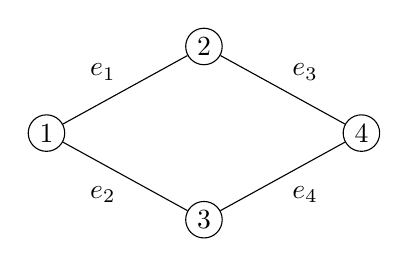
\begin{tikzpicture}[scale=1,>=stealth]
    \node[circle,draw,inner sep=1.8pt] (1) at (0,0) {$1$};
    \node[circle,draw,inner sep=1.8pt] (2) at (2,1.1) {$2$};
    \node[circle,draw,inner sep=1.8pt] (3) at (2,-1.1) {$3$};
    \node[circle,draw,inner sep=1.8pt] (4) at (4,0) {$4$};
    \draw (1) -- node[above left] {$e_1$} (2);
    \draw (1) -- node[below left] {$e_2$} (3);
    \draw (2) -- node[above right] {$e_3$} (4);
    \draw (3) -- node[below right] {$e_4$} (4);
\end{tikzpicture}
\end{center}

\begin{examplebox}[title={Reading adjacency and incidence from a graph}]
In the graph above:
\begin{itemize}[leftmargin=*]
    \item vertices \(1\) and \(2\) are adjacent;
    \item the edge \(e_1\) is incident with vertices \(1\) and \(2\);
    \item vertex \(1\) is an endpoint of \(e_1\) and \(e_2\).
\end{itemize}
Adjacency is a relation between vertices; incidence is a relation between a vertex and an edge.
\end{examplebox}

%==================================================
\subsection{Degree of a Vertex}
%==================================================

\begin{definition}{Degree}{degree-def}
Let \(G=(V,E)\) be a graph.
\begin{itemize}[leftmargin=*]
    \item The \emph{degree} of a vertex \(v\in V\), denoted \(\deg(v)\), is the number of edges incident with \(v\).
    \item The \emph{degree of the graph}, denoted \(\deg(G)\), is the maximum degree of its vertices.
    \item A vertex of degree \(0\) is called \emph{isolated}.
    \item If every vertex has degree \(k\), then the graph is called \emph{\(k\)-regular}.
\end{itemize}
If a self-loop occurs in a multigraph, it contributes \(2\) to the degree of its vertex.
\end{definition}

\begin{examplebox}[title={Degrees in the displayed graph}]
For the graph in the previous figure,
\[
\deg(1)=2,\qquad \deg(2)=2,\qquad \deg(3)=2,\qquad \deg(4)=2.
\]
Hence the graph is \(2\)-regular.
\end{examplebox}

\begin{examplebox}[title={An isolated vertex}]
If a graph contains a vertex with no incident edges at all, then that vertex has degree \(0\) and is isolated.
\end{examplebox}

\begin{commonmistake}[title={A loop contributes two, not one}]
In a multigraph, a self-loop begins and ends at the same vertex, so it contributes \(2\) to the degree count of that vertex.
\end{commonmistake}

%==================================================
\subsection{The Handshaking Lemma}
%==================================================

\begin{theorem}{Handshaking Lemma}{handshaking}
Let \(G=(V,E)\) be an undirected graph with \(m\) edges. Then
\[
\sum_{v\in V}\deg(v)=2m.
\]
\end{theorem}

\begin{proof}
Each edge has two endpoints, so each edge contributes exactly \(2\) to the total degree count of all vertices. Summing over all edges, the total contribution is \(2m\). Therefore
\[
\sum_{v\in V}\deg(v)=2m.
\]
\end{proof}

\begin{keyformula}[title={Handshaking Lemma}]
\[
2|E|=\sum_{v\in V}\deg(v).
\]
\end{keyformula}

\begin{examplebox}[title={Example 3 from the handout}]
How many edges are there in a \(6\)-regular graph with \(10\) vertices?

Let \(m\) be the number of edges. Since every vertex has degree \(6\),
\[
\sum_{v\in V}\deg(v)=10\cdot 6=60.
\]
By the Handshaking Lemma,
\[
2m=60,
\]
so
\[
\boxed{m=30.}
\]
\end{examplebox}

\begin{theorem}{Odd-degree vertices occur in even number}{odd-degree-even-count}
In every undirected graph, the number of vertices of odd degree is even.
\end{theorem}

\begin{proof}
By the Handshaking Lemma,
\[
\sum_{v\in V}\deg(v)=2|E|,
\]
which is even. The sum of all even-degree vertices is even. Therefore the sum of the odd degrees must also be even. A sum of odd integers is even if and only if there are an even number of them. Hence the number of odd-degree vertices is even.
\end{proof}

\begin{examplebox}[title={Tutorial 7, Question 4}]
Show that in a simple graph with at least two vertices, two vertices must have the same degree.

Let the graph have \(n\ge 2\) vertices. Each degree lies in the set
\[
\{0,1,2,\dots,n-1\}.
\]
However, a simple graph cannot simultaneously contain:
\begin{itemize}[leftmargin=*]
    \item a vertex of degree \(0\), and
    \item a vertex of degree \(n-1\).
\end{itemize}
Indeed, a degree-\((n-1)\) vertex is adjacent to every other vertex, so no vertex can be isolated.

Hence the \(n\) vertices can realize at most \(n-1\) distinct degree values. By the pigeonhole principle, two vertices must have the same degree.
\end{examplebox}

\begin{extension}[title={Why the Handshaking Lemma is powerful}]
The lemma turns a local quantity, degree, into a global counting identity. Many impossibility results in graph theory are obtained by showing that the degree data violate parity or edge-count constraints coming from
\[
\sum_{v\in V}\deg(v)=2|E|.
\]
\end{extension}

%==================================================
\subsection{Special Graphs}
%==================================================

\subsubsection{Complete graphs}

\begin{definition}{Complete graph}{complete-graph}
The \emph{complete graph} on \(n\) vertices, denoted \(K_n\), is the simple graph in which every pair of distinct vertices is connected by an edge.
\end{definition}

Every vertex of \(K_n\) is adjacent to all other \(n-1\) vertices. Hence \(K_n\) is \((n-1)\)-regular and
\[
|E(K_n)|=\binom{n}{2}.
\]

% First few complete graphs K1 to K4.
\begin{center}
\begin{tikzpicture}[scale=0.9]
    \node[circle,draw,inner sep=1.4pt] at (0,0) {};
    \node at (0,-1) {$K_1$};

    \begin{scope}[shift={(2.7,0)}]
        \node[circle,draw,inner sep=1.4pt] (a) at (0,0) {};
        \node[circle,draw,inner sep=1.4pt] (b) at (1.2,0) {};
        \draw (a)--(b);
        \node at (0.6,-1) {$K_2$};
    \end{scope}

    \begin{scope}[shift={(6.2,0)}]
        \node[circle,draw,inner sep=1.4pt] (a) at (0,0.75) {};
        \node[circle,draw,inner sep=1.4pt] (b) at (-0.7,-0.45) {};
        \node[circle,draw,inner sep=1.4pt] (c) at (0.7,-0.45) {};
        \draw (a)--(b)--(c)--(a);
        \node at (0,-1.2) {$K_3$};
    \end{scope}

    \begin{scope}[shift={(10.6,0)}]
        \node[circle,draw,inner sep=1.4pt] (a) at (-0.7,0.7) {};
        \node[circle,draw,inner sep=1.4pt] (b) at (0.7,0.7) {};
        \node[circle,draw,inner sep=1.4pt] (c) at (-0.7,-0.7) {};
        \node[circle,draw,inner sep=1.4pt] (d) at (0.7,-0.7) {};
        \draw (a)--(b)--(d)--(c)--(a)--(d) (b)--(c);
        \node at (0,-1.4) {$K_4$};
    \end{scope}
\end{tikzpicture}
\end{center}

\subsubsection{Cycle graphs}

\begin{definition}{Cycle graph}{cycle-graph}
For \(n\ge 3\), the \emph{cycle graph} \(C_n\) has vertices \(v_1,\dots,v_n\) and edge set
\[
\{\{v_1,v_2\},\{v_2,v_3\},\dots,\{v_{n-1},v_n\},\{v_n,v_1\}\}.
\]
\end{definition}

Every cycle graph is \(2\)-regular.

% First few cycle graphs C3 to C5.
\begin{center}
\begin{tikzpicture}[scale=0.9]
    \begin{scope}[shift={(0,0)}]
        \node[circle,draw,inner sep=1.4pt] (a) at (0,0.9) {};
        \node[circle,draw,inner sep=1.4pt] (b) at (-0.8,-0.45) {};
        \node[circle,draw,inner sep=1.4pt] (c) at (0.8,-0.45) {};
        \draw (a)--(b)--(c)--(a);
        \node at (0,-1.25) {$C_3$};
    \end{scope}
    \begin{scope}[shift={(4,0)}]
        \node[circle,draw,inner sep=1.4pt] (a) at (-0.8,0.8) {};
        \node[circle,draw,inner sep=1.4pt] (b) at (0.8,0.8) {};
        \node[circle,draw,inner sep=1.4pt] (c) at (0.8,-0.8) {};
        \node[circle,draw,inner sep=1.4pt] (d) at (-0.8,-0.8) {};
        \draw (a)--(b)--(c)--(d)--(a);
        \node at (0,-1.35) {$C_4$};
    \end{scope}
    \begin{scope}[shift={(8.5,0)}]
        \foreach \i/\x/\y in {1/0/1,2/0.95/0.3,3/0.58/-0.82,4/-0.58/-0.82,5/-0.95/0.3}
            \node[circle,draw,inner sep=1.4pt] (v\i) at (\x,\y) {};
        \draw (v1)--(v2)--(v3)--(v4)--(v5)--(v1);
        \node at (0,-1.35) {$C_5$};
    \end{scope}
\end{tikzpicture}
\end{center}

\begin{examplebox}[title={Degrees in special graphs}]
For \(K_n\), every vertex has degree \(n-1\).
For \(C_n\), every vertex has degree \(2\).
Hence
\[
\deg(K_n)=n-1,
\qquad
\deg(C_n)=2.
\]
\end{examplebox}

%==================================================
\subsection{Subgraphs and Induced Subgraphs}
%==================================================

\begin{definition}{Subgraph}{subgraph-def}
A graph \(H=(W,F)\) is a \emph{subgraph} of a graph \(G=(V,E)\) if
\[
W\subseteq V
\qquad\text{and}\qquad
F\subseteq E.
\]
\end{definition}

\begin{definition}{Induced subgraph}{induced-subgraph}
A subgraph \(H=(W,F)\) of \(G=(V,E)\) is an \emph{induced subgraph} if \(F\) contains \emph{all} edges of \(G\) whose endpoints both lie in \(W\).
\end{definition}

% Subgraph versus induced subgraph on the same vertex subset.
\begin{center}
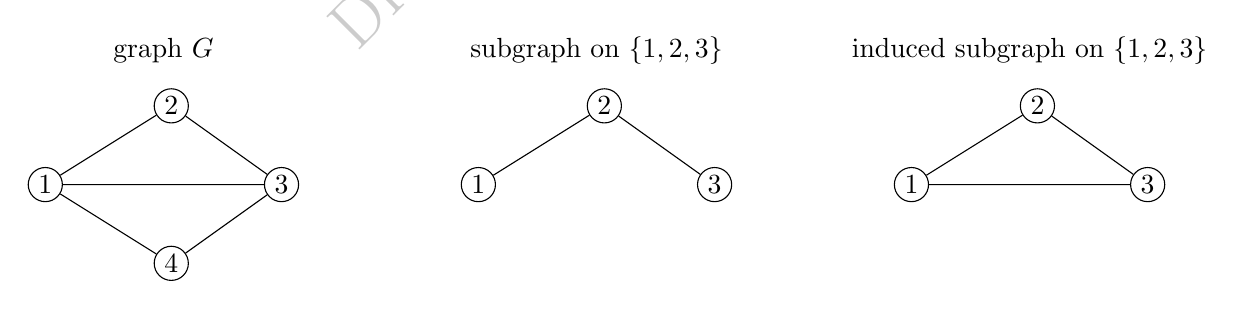
\begin{tikzpicture}[scale=1]
    \begin{scope}[shift={(0,0)}]
        \node at (1.5,1.7) {graph $G$};
        \node[circle,draw,inner sep=1.5pt] (1) at (0,0) {$1$};
        \node[circle,draw,inner sep=1.5pt] (2) at (1.6,1.0) {$2$};
        \node[circle,draw,inner sep=1.5pt] (3) at (3.0,0) {$3$};
        \node[circle,draw,inner sep=1.5pt] (4) at (1.6,-1.0) {$4$};
        \draw (1)--(2)--(3)--(4)--(1)--(3);
    \end{scope}
    \begin{scope}[shift={(5.5,0)}]
        \node at (1.5,1.7) {subgraph on $\{1,2,3\}$};
        \node[circle,draw,inner sep=1.5pt] (1) at (0,0) {$1$};
        \node[circle,draw,inner sep=1.5pt] (2) at (1.6,1.0) {$2$};
        \node[circle,draw,inner sep=1.5pt] (3) at (3.0,0) {$3$};
        \draw (1)--(2)--(3);
    \end{scope}
    \begin{scope}[shift={(11,0)}]
        \node at (1.5,1.7) {induced subgraph on $\{1,2,3\}$};
        \node[circle,draw,inner sep=1.5pt] (1) at (0,0) {$1$};
        \node[circle,draw,inner sep=1.5pt] (2) at (1.6,1.0) {$2$};
        \node[circle,draw,inner sep=1.5pt] (3) at (3.0,0) {$3$};
        \draw (1)--(2)--(3)--(1);
    \end{scope}
\end{tikzpicture}
\end{center}

\begin{examplebox}[title={Subgraph versus induced subgraph}]
Choose vertices \(\{1,2,3\}\) from the graph displayed above. If one keeps only some of the edges among these three vertices, one gets a subgraph. If one keeps \emph{all} edges of the original graph between these chosen vertices, one gets the induced subgraph.
\end{examplebox}

\begin{commonmistake}[title={Not every subgraph is induced}]
An induced subgraph is determined entirely by its vertex subset. A general subgraph is not: after choosing vertices, one may still omit edges that were present in the original graph.
\end{commonmistake}

%==================================================
\subsection{Graph Isomorphism}
%==================================================

\begin{definition}{Graph isomorphism}{graph-isomorphism}
Two undirected graphs
\[
G_1=(V_1,E_1)
\qquad\text{and}\qquad
G_2=(V_2,E_2)
\]
are \emph{isomorphic} if there exists a bijection
\[
f:V_1\to V_2
\]
such that for all \(u,v\in V_1\),
\[
\{u,v\}\in E_1
\iff
\{f(u),f(v)\}\in E_2.
\]
\end{definition}

Intuitively, isomorphic graphs are the same graph with different vertex labels.

\begin{examplebox}[title={A concrete isomorphism}]
Let
\[
V_1=\{a,b,c,d\},
\qquad
V_2=\{r,s,t,u\},
\]
and suppose the edges in the two graphs correspond as follows:
\[
f(a)=r,\qquad f(b)=s,\qquad f(c)=u,\qquad f(d)=t.
\]
If adjacency is preserved under this bijection, then the graphs are isomorphic.
\end{examplebox}

\begin{examtip}[title={How to prove two graphs are isomorphic}]
To prove two graphs are isomorphic, one must produce an explicit bijection between their vertex sets and check that adjacency is preserved in both directions.
\end{examtip}

\subsubsection{Graph invariants}

A \emph{graph invariant} is a property preserved by isomorphism. Common invariants include:
\begin{itemize}[leftmargin=*]
    \item number of vertices;
    \item number of edges;
    \item number of isolated vertices;
    \item degree sequence;
    \item regularity.
\end{itemize}

\begin{examplebox}[title={Showing graphs are not isomorphic}]
If one graph has degree sequence
\[
(3,2,2,1)
\]
and another has degree sequence
\[
(3,3,1,1),
\]
then the graphs cannot be isomorphic, because degree sequence is an invariant.
\end{examplebox}

\begin{examplebox}[title={Handout non-isomorphism example}]
The handout gives a pair of graphs \(G\) and \(H\) and notes that a vertex of degree \(2\) in \(G\) is adjacent to two vertices of degree \(3\), while no degree-\(2\) vertex in \(H\) has that property. Hence the graphs are not isomorphic.

This illustrates a common strategy: compare \emph{local adjacency patterns} among vertices of the same degree.
\end{examplebox}

\begin{extension}[title={Why isomorphism can be difficult}]
For two graphs with \(n\) vertices there are \(n!\) possible bijections between the vertex sets. Brute-force checking is therefore impractical even for moderate \(n\). In practice one first uses invariants to rule out isomorphism quickly, and only then searches for an explicit bijection if the invariants are compatible.
\end{extension}

%==================================================
\subsection{Special Techniques}
%==================================================

\subsubsection*{1. Ignore the picture, read the adjacency}
Different drawings can represent the same graph. Always extract the vertex set and edge set, not the visual layout.

\subsubsection*{2. Use the Handshaking Lemma early}
Whenever degrees and edge counts appear together, immediately consider
\[
\sum_{v\in V}\deg(v)=2|E|.
\]
This often gives the shortest solution.

\subsubsection*{3. Use invariants to disprove isomorphism}
To show two graphs are not isomorphic, compare quick invariants such as:
\begin{itemize}[leftmargin=*]
    \item number of vertices;
    \item number of edges;
    \item degree sequence;
    \item number of isolated vertices;
    \item adjacency pattern among high-degree vertices.
\end{itemize}

\subsubsection*{4. For isomorphism, build a bijection strategically}
Match vertices of uncommon degree first. Then check whether their neighborhoods correspond.

\subsubsection*{5. Distinguish subgraph from induced subgraph}
A subgraph may omit edges. An induced subgraph may not omit any edge whose endpoints remain in the chosen vertex set.

\subsubsection*{6. Check parity of odd degrees}
If a proposed degree pattern contains an odd number of odd entries, then it cannot come from any graph.

\begin{examtip}[title={Fast diagnostic summary}]
When facing a graph question, ask in this order:
\begin{enumerate}[leftmargin=*]
    \item Is the graph simple or directed?
    \item What are \(|V|\) and \(|E|\)?
    \item What are the degrees of the vertices?
    \item Can the Handshaking Lemma be applied?
    \item Is the task about equality of drawings, or about isomorphism of abstract graphs?
\end{enumerate}
\end{examtip}

%==================================================
\subsection{Summary Table}
%==================================================

\begin{center}
\small
\begin{tabular}{@{}p{0.27\textwidth}p{0.28\textwidth}p{0.34\textwidth}@{}}
\toprule
\textbf{Concept} & \textbf{Formal object} & \textbf{Key point} \\
\midrule
Undirected graph & \(G=(V,E)\) with edges as unordered pairs & adjacency is symmetric \\
Directed graph & \(G=(V,E)\) with edges as ordered pairs & direction matters \\
Simple graph & no loops, no multiple edges & \(0\le |E|\le \binom{|V|}{2}\) \\
Degree & \(\deg(v)\) & number of incident edges \\
Regular graph & all vertices same degree & \(k\)-regular means \(\deg(v)=k\) for all \(v\) \\
Handshaking Lemma & \(2|E|=\sum_{v\in V}\deg(v)\) & total degree count is even \\
Complete graph & \(K_n\) & every pair of vertices adjacent \\
Cycle graph & \(C_n\) & every vertex has degree \(2\) \\
Subgraph & \(W\subseteq V,\ F\subseteq E\) & may omit edges \\
Induced subgraph & determined by chosen vertex subset & keeps all edges among chosen vertices \\
Isomorphism & adjacency-preserving bijection & same abstract graph, different labels \\
\bottomrule
\end{tabular}
\end{center}

\begin{commonmistake}[title={Final warning for Handout 07}]
A graph question is rarely about the artistic appearance of a drawing. It is about the combinatorial structure: which vertices are present, which edges are present, and how these determine adjacency, degree, and isomorphism.
\end{commonmistake}}{}
\IfFileExists{chapters/handout08.tex}{% Source reference: :contentReference[oaicite:0]{index=0}
\part{Graph Theory}
\section{Handout 08: Graph Theory (2): Traversing Graphs}

\subsection{Overview}

This handout studies how to traverse graphs. The main objects are paths, circuits, connectivity, Euler paths/circuits, and Hamilton paths/circuits.

The central distinction is:
\[
\text{Euler: use every edge exactly once}
\qquad\text{versus}\qquad
\text{Hamilton: visit every vertex exactly once}.
\]

The main topics are:
\begin{itemize}[leftmargin=*]
    \item directed graphs and in-degree/out-degree;
    \item directed Handshaking Lemma;
    \item paths, simple paths, circuits, and length;
    \item connected components in undirected graphs;
    \item strongly and weakly connected directed graphs;
    \item Euler circuits and Euler paths;
    \item Hamilton circuits and Hamilton paths.
\end{itemize}

\begin{examtip}[title={Main diagnostic for Handout 08}]
Before solving a traversing-graph problem, decide whether the condition is about:
\[
\text{reachability},\qquad
\text{using edges},\qquad
\text{visiting vertices}.
\]
Connectivity is about reachability, Euler theory is about edges, and Hamilton theory is about vertices.
\end{examtip}

%==================================================
\subsection{Directed Graphs and Directed Degree}
%==================================================

\begin{definition}{Directed graph}{directed-graph-recall}
A graph \(G=(V,E)\) is \emph{directed} if every edge in \(E\) is an ordered pair of vertices. An edge
\[
e=(u,v)
\]
has direction from \(u\) to \(v\). The vertex \(u\) is the \emph{initial vertex} of \(e\), and \(v\) is the \emph{terminal vertex} of \(e\).
\end{definition}

\begin{definition}{In-degree and out-degree}{directed-degree}
Let \(G=(V,E)\) be a directed graph.
\begin{itemize}[leftmargin=*]
    \item The \emph{in-degree} of a vertex \(v\), denoted \(\deg^{-}(v)\), is the number of directed edges whose terminal vertex is \(v\).
    \item The \emph{out-degree} of a vertex \(v\), denoted \(\deg^{+}(v)\), is the number of directed edges whose initial vertex is \(v\).
\end{itemize}
A self-loop at \(v\) contributes \(1\) to \(\deg^{-}(v)\) and \(1\) to \(\deg^{+}(v)\).
\end{definition}

% Directed graph illustrating in-degrees and out-degrees.
\begin{center}
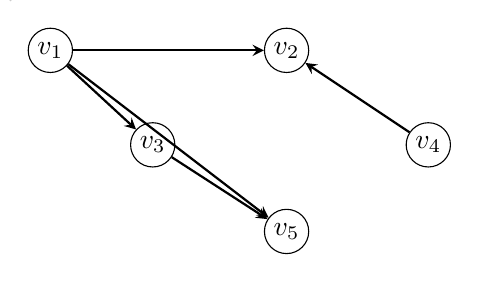
\begin{tikzpicture}[>=stealth,scale=1.0]
    \node[circle,draw,inner sep=1.8pt] (v1) at (0,1.2) {$v_1$};
    \node[circle,draw,inner sep=1.8pt] (v2) at (3,1.2) {$v_2$};
    \node[circle,draw,inner sep=1.8pt] (v3) at (1.3,0) {$v_3$};
    \node[circle,draw,inner sep=1.8pt] (v5) at (3.0,-1.1) {$v_5$};
    \node[circle,draw,inner sep=1.8pt] (v4) at (4.8,0) {$v_4$};

    \draw[->,thick] (v1) -- (v2);
    \draw[->,thick] (v1) -- (v3);
    \draw[->,thick] (v1) -- (v5);
    \draw[->,thick] (v4) -- (v2);
    \draw[->,thick] (v3) -- (v5);
\end{tikzpicture}
\end{center}

\begin{examplebox}[title={Directed degree calculation}]
For the directed graph with
\[
V=\{v_1,v_2,v_3,v_4,v_5\}
\]
and
\[
E=\{(v_1,v_2),(v_1,v_3),(v_1,v_5),(v_4,v_2),(v_3,v_5)\},
\]
the degrees are:
\[
\deg^{-}(v_1)=0,\quad \deg^{+}(v_1)=3,
\]
\[
\deg^{-}(v_2)=2,\quad \deg^{+}(v_2)=0,
\]
\[
\deg^{-}(v_3)=1,\quad \deg^{+}(v_3)=1,
\]
\[
\deg^{-}(v_4)=0,\quad \deg^{+}(v_4)=1,
\]
\[
\deg^{-}(v_5)=2,\quad \deg^{+}(v_5)=0.
\]
\end{examplebox}

\begin{theorem}{Directed Handshaking Lemma}{directed-handshaking}
Let \(G=(V,E)\) be a directed graph with \(m\) edges. Then
\[
\sum_{v\in V}\deg^{-}(v)
=
\sum_{v\in V}\deg^{+}(v)
=
m.
\]
\end{theorem}

\begin{proof}
Each directed edge has exactly one initial vertex and exactly one terminal vertex. Hence each edge contributes \(1\) to the total out-degree and \(1\) to the total in-degree. Summing over all \(m\) edges gives the result.
\end{proof}

\begin{keyformula}[title={Directed Handshaking Lemma}]
\[
\sum_{v\in V}\deg^{-}(v)=\sum_{v\in V}\deg^{+}(v)=|E|.
\]
\end{keyformula}

\begin{commonmistake}[title={Undirected degree versus directed degree}]
In an undirected graph, one edge contributes \(2\) to the total degree sum. In a directed graph, one directed edge contributes \(1\) to the total in-degree and \(1\) to the total out-degree separately.
\end{commonmistake}

%==================================================
\subsection{Paths, Simple Paths, and Circuits}
%==================================================

\begin{definition}{Path in an undirected graph}{undirected-path}
Let \(G=(V,E)\) be an undirected graph. A \emph{path} from \(u\) to \(v\) is a sequence of vertices
\[
(u=w_0,w_1,\dots,w_k,w_{k+1}=v)
\]
such that
\[
\{w_i,w_{i+1}\}\in E
\qquad
\text{for all }0\le i\le k.
\]
The \emph{length} of the path is the number of edges in the path.
\end{definition}

\begin{definition}{Path in a directed graph}{directed-path}
Let \(G=(V,E)\) be a directed graph. A \emph{directed path} from \(u\) to \(v\) is a sequence of vertices
\[
(u=w_0,w_1,\dots,w_k,w_{k+1}=v)
\]
such that
\[
(w_i,w_{i+1})\in E
\qquad
\text{for all }0\le i\le k.
\]
The direction of every edge must match the order in the vertex sequence.
\end{definition}

\begin{definition}{Simple path and circuit}{simple-path-circuit}
In this course, a \emph{simple path} is a path that contains no edge more than once.

If a path starts and ends at the same vertex, then it is called a \emph{circuit}.
\end{definition}

\begin{examtip}[title={Course convention for simple path}]
Some books define a simple path as one with no repeated vertices. In this course, the relevant definition is: \emph{no edge is repeated}. Use the course definition unless a question explicitly states otherwise.
\end{examtip}

% Graph for path and circuit examples.
\begin{center}
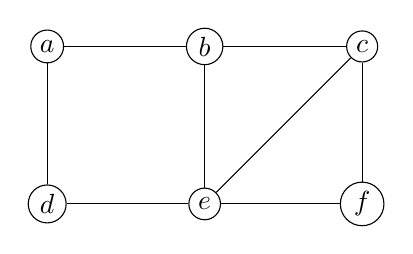
\begin{tikzpicture}[scale=1.0]
    \node[circle,draw,inner sep=1.8pt] (a) at (0,1) {$a$};
    \node[circle,draw,inner sep=1.8pt] (b) at (2,1) {$b$};
    \node[circle,draw,inner sep=1.8pt] (c) at (4,1) {$c$};
    \node[circle,draw,inner sep=1.8pt] (d) at (0,-1) {$d$};
    \node[circle,draw,inner sep=1.8pt] (e) at (2,-1) {$e$};
    \node[circle,draw,inner sep=1.8pt] (f) at (4,-1) {$f$};

    \draw (a)--(b)--(c)--(f)--(e)--(d)--(a);
    \draw (b)--(e);
    \draw (c)--(e);
\end{tikzpicture}
\end{center}

\begin{examplebox}[title={Reading paths from a graph}]
In the graph above:
\begin{itemize}[leftmargin=*]
    \item \(d-a-b-c-f\) is a simple path of length \(4\);
    \item \(d-e-c-b-a-d\) is a circuit of length \(5\);
    \item \(a-b,e-f\) is not a path, since there is no edge joining \(b\) to \(e\) in that sequence unless \(b-e\) is explicitly present;
    \item \(d-a-b-c-f-b-a-e\) would fail to be simple if an edge is reused.
\end{itemize}
\end{examplebox}

\begin{commonmistake}[title={A sequence of vertices is not automatically a path}]
A vertex sequence is a path only if every consecutive pair is joined by the required edge. In a directed graph, the edge direction must also agree with the order of the sequence.
\end{commonmistake}

%==================================================
\subsection{Connectivity}
%==================================================

\begin{definition}{Connected graph and components}{connected-components}
An undirected graph \(G=(V,E)\) is \emph{connected} if for every pair of vertices \(u,v\in V\), there is a path from \(u\) to \(v\).

If \(G\) is not connected, it is called \emph{disconnected}. Its maximal connected subgraphs are called its \emph{connected components}.
\end{definition}

% Connected versus disconnected graph.
\begin{center}
\begin{tikzpicture}[scale=1.0]
    \begin{scope}[shift={(0,0)}]
        \node at (1.8,1.7) {connected};
        \node[circle,draw,inner sep=1.5pt] (a) at (0,0) {};
        \node[circle,draw,inner sep=1.5pt] (b) at (1.2,1) {};
        \node[circle,draw,inner sep=1.5pt] (c) at (2.4,0) {};
        \node[circle,draw,inner sep=1.5pt] (d) at (1.2,-1) {};
        \draw (a)--(b)--(c)--(d)--(a);
        \draw (b)--(d);
    \end{scope}

    \begin{scope}[shift={(6,0)}]
        \node at (1.8,1.7) {disconnected};
        \node[circle,draw,inner sep=1.5pt] (a) at (0,0) {};
        \node[circle,draw,inner sep=1.5pt] (b) at (1,0.8) {};
        \node[circle,draw,inner sep=1.5pt] (c) at (1,-0.8) {};
        \draw (a)--(b)--(c)--(a);

        \node[circle,draw,inner sep=1.5pt] (d) at (3.2,0.5) {};
        \node[circle,draw,inner sep=1.5pt] (e) at (4.2,0.5) {};
        \draw (d)--(e);
    \end{scope}
\end{tikzpicture}
\end{center}

\begin{theorem}{Existence of simple paths in connected graphs}{connected-simple-path}
There is a simple path between every pair of distinct vertices in a connected graph.
\end{theorem}

\begin{proof}
Let \(u\) and \(v\) be distinct vertices in a connected graph \(G\). Since \(G\) is connected, there exists at least one path from \(u\) to \(v\).

Choose a path from \(u\) to \(v\) of minimum length. If this path repeated an edge, then the repeated portion could be bypassed to produce a shorter path from \(u\) to \(v\), contradicting the minimality of the chosen path. Therefore the chosen path contains no repeated edge and is simple.
\end{proof}

\begin{extension}[title={Shortest path as a simplification device}]
The theorem uses a standard graph-theoretic trick: choose a shortest object among all possible objects. Minimality then forces unnecessary repetitions to disappear.
\end{extension}

%==================================================
\subsection{Strong and Weak Connectivity in Directed Graphs}
%==================================================

\begin{definition}{Strongly connected directed graph}{strong-connected}
A directed graph \(G=(V,E)\) is \emph{strongly connected} if for every pair of vertices \(u,v\in V\), there is a directed path from \(u\) to \(v\) and a directed path from \(v\) to \(u\).
\end{definition}

\begin{definition}{Weakly connected directed graph}{weak-connected}
A directed graph \(G=(V,E)\) is \emph{weakly connected} if its underlying undirected graph is connected. The underlying undirected graph is obtained by removing the directions from all directed edges.
\end{definition}

Strong connectivity implies weak connectivity, but the converse need not hold.

\begin{examplebox}[title={Tutorial 8, Question 1}]
Consider the directed graph with
\[
V=\{a,b,c,d,e\},
\qquad
E=\{(b,a),(b,c),(b,e),(e,a),(d,b),(c,d)\}.
\]
It is not strongly connected, since \(a\) has out-degree \(0\), so there is no directed path from \(a\) to any other vertex.

However, after ignoring directions, the underlying undirected graph has edges
\[
\{a,b\},\{b,c\},\{b,e\},\{a,e\},\{b,d\},\{c,d\},
\]
which form a connected undirected graph. Hence the digraph is weakly connected but not strongly connected.
\end{examplebox}

\begin{examplebox}[title={A graph that is not weakly connected}]
If a directed graph has underlying undirected connected components
\[
\{a,c,d,g\}
\qquad\text{and}\qquad
\{b,e,f\},
\]
then it is not weakly connected. Therefore it is also not strongly connected.
\end{examplebox}

\begin{commonmistake}[title={Checking only one direction of reachability}]
For strong connectivity, it is not enough to check that every vertex can be reached from one starting vertex. One also needs directed reachability in the reverse direction for every pair.
\end{commonmistake}

\begin{examtip}[title={Fast strong/weak connectivity test}]
For a directed graph:
\begin{enumerate}[leftmargin=*]
    \item first ignore directions and test weak connectivity;
    \item if weak connectivity fails, strong connectivity is impossible;
    \item if weak connectivity holds, then test directed reachability.
\end{enumerate}
\end{examtip}

%==================================================
\subsection{Euler Circuits and Euler Paths}
%==================================================

The Euler problem asks whether a graph can be traversed using each edge exactly once.

\begin{definition}{Euler circuit and Euler path}{euler-def}
Let \(G\) be a connected undirected graph.
\begin{itemize}[leftmargin=*]
    \item An \emph{Euler circuit} in \(G\) is a simple circuit containing every edge of \(G\).
    \item An \emph{Euler path} in \(G\) is a simple path containing every edge of \(G\).
\end{itemize}
\end{definition}

\begin{theorem}{Euler circuit criterion}{euler-circuit}
A connected graph \(G\) with at least two vertices has an Euler circuit if and only if every vertex of \(G\) has even degree.
\end{theorem}

\begin{proof}
\textbf{Only if.}
Suppose \(G\) has an Euler circuit. Every time the circuit enters a vertex, it must leave along a different unused edge. Thus edges incident with each vertex are paired as ``enter'' and ``leave'' edges. Since the circuit is closed, this also holds at the starting vertex. Hence every vertex has even degree.

\textbf{If.}
Suppose every vertex has even degree. Start at any vertex and follow unused edges as long as possible. Since each time one enters a non-starting vertex there remains an unused edge to leave by, the path cannot get stuck away from its starting vertex. Hence it closes into a circuit.

If this circuit does not yet use all edges, then because the graph is connected, some vertex on the circuit is incident with an unused edge. Starting from that vertex, construct another closed circuit in the remaining unused edges and splice it into the first circuit. Repeating this process eventually uses every edge, producing an Euler circuit.
\end{proof}

\begin{keyformula}[title={Euler circuit test}]
For a connected graph:
\[
\text{Euler circuit exists}
\quad\Longleftrightarrow\quad
\text{all vertices have even degree}.
\]
\end{keyformula}

% Splicing two circuits in the proof of Euler's circuit theorem.
\begin{center}
\begin{tikzpicture}[scale=1.0]
    \node[circle,draw,inner sep=1.5pt,label=below:{\(v\)}] (v) at (0,0) {};
    \draw (v) .. controls (-1.5,1.2) and (-2,-1.2) .. (v);
    \draw (v) .. controls (1.5,1.0) and (2,-1.0) .. (v);
    \node at (-1.6,0) {\(C_1\)};
    \node at (1.6,0) {\(C_2\)};
\end{tikzpicture}
\end{center}

\begin{examplebox}[title={Tutorial 8, Question 4}]
Suppose a connected graph has degrees
\[
4,4,6,4,4,2,4,6,4.
\]
Every degree is even. Therefore, by the Euler circuit criterion, the graph has an Euler circuit.
\end{examplebox}

\begin{theorem}{Euler path criterion}{euler-path}
A connected graph \(G\) has an Euler path but not an Euler circuit if and only if \(G\) has exactly two vertices of odd degree.
\end{theorem}

\begin{proof}
\textbf{Only if.}
Suppose \(G\) has an Euler path that is not a circuit. Let the path start at \(u\) and end at \(v\), with \(u\neq v\). Every internal vertex is entered and left the same number of times, so it has even degree. The starting vertex \(u\) is left one more time than it is entered, and the ending vertex \(v\) is entered one more time than it is left. Hence \(u\) and \(v\) are the only odd-degree vertices.

\textbf{If.}
Suppose \(G\) has exactly two odd-degree vertices \(u\) and \(v\). Add one new edge between \(u\) and \(v\). Now every vertex has even degree, so the new graph has an Euler circuit. Removing the added edge from this circuit produces an Euler path in the original graph, starting at one of \(u,v\) and ending at the other.
\end{proof}

\begin{keyformula}[title={Euler path test}]
For a connected graph:
\[
\begin{array}{c|c}
\text{number of odd-degree vertices} & \text{Euler conclusion} \\ \hline
0 & \text{Euler circuit exists} \\
2 & \text{Euler path but no Euler circuit} \\
\text{other} & \text{no Euler path}
\end{array}
\]
\end{keyformula}

\begin{examplebox}[title={One-stroke drawing criterion}]
A connected drawing can be traced in one continuous stroke without retracing an edge if and only if its corresponding graph has either:
\begin{itemize}[leftmargin=*]
    \item \(0\) odd-degree vertices, giving a closed one-stroke drawing; or
    \item \(2\) odd-degree vertices, giving an open one-stroke drawing.
\end{itemize}
If there are more than two odd-degree vertices, such a drawing is impossible.
\end{examplebox}

\begin{examplebox}[title={Tutorial 8, Question 7}]
For the complete graph \(K_n\), every vertex has degree \(n-1\). Since \(K_n\) is connected, it has an Euler circuit exactly when \(n-1\) is even, i.e.
\[
\boxed{n\text{ is odd}.}
\]

For the cycle graph \(C_n\), every vertex has degree \(2\), so every \(C_n\) with \(n\ge 3\) has an Euler circuit.
\[
\boxed{C_n\text{ has an Euler circuit for all }n\ge 3.}
\]
\end{examplebox}

\begin{commonmistake}[title={Ignoring connectedness in Euler criteria}]
The degree conditions are not enough if the graph is disconnected. Euler path and circuit criteria in this handout apply to connected graphs.
\end{commonmistake}

\begin{extension}[title={Why odd vertices are endpoints}]
In an Euler path, every internal visit to a vertex uses incident edges in pairs: one edge to enter and one edge to leave. Only the start and end vertices can have unpaired incident edges. This explains why Euler paths have exactly two odd vertices when they are not circuits.
\end{extension}

%==================================================
\subsection{Hamilton Paths and Hamilton Circuits}
%==================================================

Hamilton problems ask whether a graph can visit every vertex exactly once.

\begin{definition}{Hamilton path and Hamilton circuit}{hamilton-def}
Let \(G=(V,E)\) be a graph.
\begin{itemize}[leftmargin=*]
    \item A \emph{Hamilton path} is a path in \(G\) that visits every vertex exactly once.
    \item A \emph{Hamilton circuit} is a circuit in \(G\) that visits every vertex exactly once, except that the starting vertex is repeated at the end to close the circuit.
\end{itemize}
\end{definition}

\begin{keyformula}[title={Euler versus Hamilton}]
\[
\begin{array}{c|c}
\text{Euler} & \text{uses every edge exactly once} \\
\text{Hamilton} & \text{visits every vertex exactly once}
\end{array}
\]
\end{keyformula}

\begin{examplebox}[title={Tutorial 8, Question 8}]
In the graph with vertices \(A,B,C,D,E\) and edges including
\[
AB,\ BC,\ CD,\ DE,\ EA,
\]
the sequence
\[
A\to B\to C\to D\to E\to A
\]
is a Hamilton circuit because it visits every vertex exactly once before returning to the start.
\end{examplebox}

\begin{examplebox}[title={Bridge obstruction to a Hamilton circuit}]
If a graph consists of two triangles connected by a single bridge edge \(cf\), then it has no Hamilton circuit. A Hamilton circuit would need to cross from one triangle to the other and later return, but the only connecting edge is \(cf\). Using it twice is impossible in a circuit that visits each vertex exactly once.
\end{examplebox}

\begin{commonmistake}[title={Using Euler criteria for Hamilton problems}]
Even degrees do not guarantee a Hamilton circuit, and odd degrees do not automatically rule one out. Euler criteria are edge-based; Hamilton questions are vertex-based.
\end{commonmistake}

\begin{examtip}[title={How Hamilton problems are usually handled}]
Unlike Euler paths and circuits, Hamilton paths and circuits do not have a simple degree-parity test in this handout. Typical solutions either:
\begin{itemize}[leftmargin=*]
    \item exhibit an explicit Hamilton path or circuit; or
    \item prove impossibility using a structural obstruction such as a bridge, forced vertex, or separation.
\end{itemize}
\end{examtip}

\begin{extension}[title={Why Hamilton problems are harder}]
A graph with \(n\) vertices has up to \(n!\) possible vertex orderings to test as candidate Hamilton paths. This factorial search space explains why Hamilton path and circuit problems are substantially harder than Euler problems, where degree criteria give a fast test.
\end{extension}

%==================================================
\subsection{Euler versus Hamilton: Structural Comparison}
%==================================================

\begin{center}
\small
\begin{tabular}{@{}p{0.25\textwidth}p{0.30\textwidth}p{0.32\textwidth}@{}}
\toprule
\textbf{Concept} & \textbf{What must be used?} & \textbf{Fast test in this handout?} \\
\midrule
Euler path & every edge exactly once & yes: connected and exactly \(0\) or \(2\) odd vertices \\
Euler circuit & every edge exactly once and return to start & yes: connected and all vertices even \\
Hamilton path & every vertex exactly once & no simple degree-parity test \\
Hamilton circuit & every vertex exactly once and return to start & no simple degree-parity test \\
\bottomrule
\end{tabular}
\end{center}

\begin{examtip}[title={Fast classification}]
If the question says ``draw without lifting pencil or retracing'', think Euler. If the question says ``visit each vertex exactly once'', think Hamilton.
\end{examtip}

%==================================================
\subsection{Special Techniques}
%==================================================

\subsubsection*{1. Use the underlying graph for weak connectivity}
For a directed graph, ignore all arrow directions and test whether the resulting undirected graph is connected.

\subsubsection*{2. Use reachability for strong connectivity}
Strong connectivity requires directed paths both ways between every pair of vertices. Vertices with out-degree \(0\) or in-degree \(0\) are immediate obstructions unless the graph has only one vertex.

\subsubsection*{3. Replace arbitrary paths by shortest paths}
In connected graphs, shortest paths are automatically simple under the course definition. This is useful for proofs involving minimality.

\subsubsection*{4. Count odd-degree vertices for Euler questions}
For a connected graph:
\[
0\text{ odd vertices}\Rightarrow \text{Euler circuit},
\qquad
2\text{ odd vertices}\Rightarrow \text{Euler path only}.
\]

\subsubsection*{5. Add an edge between two odd vertices}
To prove the Euler path criterion, add an edge between the two odd-degree vertices to create an Euler circuit, then remove that added edge.

\subsubsection*{6. Use bridges as Hamilton obstructions}
A Hamilton circuit cannot rely on a bridge to connect two parts of a graph, because a circuit would need a way to return without revisiting vertices.

\subsubsection*{7. Exhibit Hamilton circuits explicitly}
To prove that a Hamilton circuit exists, it is enough to list a cyclic order of vertices and check that every consecutive pair is connected by an edge.

\begin{extension}[title={Traversal problem decision tree}]
A useful decision tree is:
\[
\begin{array}{c|c}
\text{Requirement} & \text{Method} \\ \hline
\text{reach every vertex from every other} & \text{connectivity / strong connectivity} \\
\text{use every edge exactly once} & \text{Euler degree test} \\
\text{visit every vertex exactly once} & \text{construct or obstruct Hamilton path/circuit}
\end{array}
\]
This prevents applying Euler's theorem to Hamilton questions.
\end{extension}

%==================================================
\subsection{Summary Table}
%==================================================

\begin{center}
\small
\begin{tabular}{@{}p{0.27\textwidth}p{0.30\textwidth}p{0.32\textwidth}@{}}
\toprule
\textbf{Concept} & \textbf{Definition / criterion} & \textbf{Exam use} \\
\midrule
In-degree & number of incoming directed edges & compute terminal-edge counts \\
Out-degree & number of outgoing directed edges & detect directed reachability obstruction \\
Directed handshaking & \(\sum\deg^-=\sum\deg^+=|E|\) & check directed degree totals \\
Path & consecutive vertices joined by edges & prove reachability \\
Circuit & path beginning and ending at same vertex & closed traversal \\
Connected graph & path between every pair of vertices & undirected reachability \\
Strongly connected & directed paths both ways between all pairs & directed reachability \\
Weakly connected & underlying undirected graph connected & ignore arrows first \\
Euler circuit & uses every edge exactly once and closes & connected + all degrees even \\
Euler path & uses every edge exactly once & connected + \(0\) or \(2\) odd vertices \\
Hamilton circuit & visits every vertex exactly once and closes & usually construct or prove obstruction \\
Hamilton path & visits every vertex exactly once & no simple degree-parity test \\
\bottomrule
\end{tabular}
\end{center}

\begin{commonmistake}[title={Final warning for Handout 08}]
Do not confuse edge traversal with vertex visitation. Euler questions are controlled by edge degrees; Hamilton questions are controlled by global vertex-order structure and usually require direct construction or a structural obstruction.
\end{commonmistake}}{}
\IfFileExists{chapters/handout09.tex}{% Source reference: :contentReference[oaicite:0]{index=0}
\part{Graph Theory}
\section{Handout 09: Graph Theory (3): Graph Coloring, Planar Graphs}

\subsection{Overview}

This handout studies two major graph-theoretic themes:
\begin{itemize}[leftmargin=*]
    \item \emph{vertex coloring}: assigning colors to vertices so that adjacent vertices receive different colors;
    \item \emph{planarity}: drawing graphs in the plane without edge crossings.
\end{itemize}

The key topics are:
\begin{itemize}[leftmargin=*]
    \item \(k\)-vertex-colorings and chromatic number \(\chi(G)\);
    \item bipartite graphs as exactly the graphs that are \(2\)-colorable;
    \item complete bipartite graphs \(K_{m,n}\);
    \item planar representations and regions;
    \item Euler's formula for connected planar graphs;
    \item edge-count tests for non-planarity;
    \item non-planarity of \(K_5\) and \(K_{3,3}\);
    \item map coloring and the Four-Color Theorem.
\end{itemize}

\begin{examtip}[title={Main diagnostic for Handout 09}]
When facing a problem from this handout, first decide whether it is asking about:
\[
\begin{aligned}
&\text{coloring vertices}, && \text{splitting vertices into two parts},\\
&\text{drawing without crossings}, && \text{proving non-planarity}.
\end{aligned}
\]
These require different tools.
\end{examtip}

%==================================================
\subsection{Vertex Coloring}
%==================================================

\begin{definition}{\(k\)-vertex-coloring}{vertex-coloring}
Let \(G=(V,E)\) be a graph. A \emph{\(k\)-vertex-coloring} of \(G\) is a function
\[
f:V\to \{1,2,\dots,k\}
\]
such that whenever \(u\) and \(v\) are adjacent,
\[
\{u,v\}\in E
\quad\Longrightarrow\quad
f(u)\neq f(v).
\]
\end{definition}

Thus adjacent vertices must receive different colors. Non-adjacent vertices may receive the same color.

\begin{definition}{\(k\)-colorable graph and chromatic number}{chromatic-number}
A graph \(G\) is \emph{\(k\)-colorable} if it has a \(k\)-vertex-coloring.

The \emph{chromatic number} of \(G\), denoted \(\chi(G)\), is the smallest integer \(k\) such that \(G\) is \(k\)-colorable.
\end{definition}

\begin{keyformula}[title={Meaning of chromatic number}]
\[
\chi(G)=\min\{k:\ G\text{ has a valid }k\text{-vertex-coloring}\}.
\]
\end{keyformula}

% Example of a proper 4-coloring of a small graph.
\begin{center}
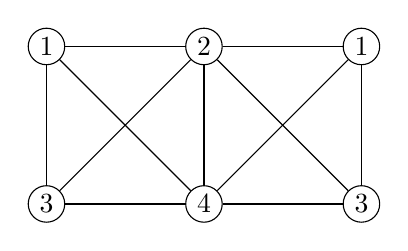
\begin{tikzpicture}[scale=1.0]
    \node[circle,draw,inner sep=1.8pt] (a) at (0,1) {$1$};
    \node[circle,draw,inner sep=1.8pt] (b) at (2,1) {$2$};
    \node[circle,draw,inner sep=1.8pt] (c) at (4,1) {$1$};
    \node[circle,draw,inner sep=1.8pt] (d) at (0,-1) {$3$};
    \node[circle,draw,inner sep=1.8pt] (e) at (2,-1) {$4$};
    \node[circle,draw,inner sep=1.8pt] (f) at (4,-1) {$3$};

    \draw (a)--(b)--(c);
    \draw (d)--(e)--(f);
    \draw (a)--(d);
    \draw (b)--(e);
    \draw (c)--(f);
    \draw (a)--(e);
    \draw (b)--(d);
    \draw (b)--(f);
    \draw (c)--(e);
\end{tikzpicture}
\end{center}

\begin{examplebox}[title={Basic chromatic numbers}]
For complete graphs,
\[
\chi(K_n)=n,
\]
because every pair of vertices is adjacent.

For cycle graphs,
\[
\chi(C_n)=
\begin{cases}
2, & n\text{ even},\\
3, & n\text{ odd}.
\end{cases}
\]
Also,
\[
\chi(G)=1
\]
if and only if \(G\) has no edges.
\end{examplebox}

\begin{proof}
For \(K_n\), every pair of vertices is adjacent, so all \(n\) vertices must receive distinct colors. Hence \(\chi(K_n)=n\).

For \(C_n\), if \(n\) is even, alternate two colors around the cycle. If \(n\) is odd, two colors cannot close consistently around the cycle, but three colors suffice. Thus the stated formula holds.
\end{proof}

\begin{commonmistake}[title={Color labels are arbitrary}]
A coloring is not about the names of colors. If two colorings differ only by renaming colors, they represent the same coloring structure. What matters is whether adjacent vertices have different colors.
\end{commonmistake}

%==================================================
\subsection{Bipartite Graphs}
%==================================================

\begin{definition}{Bipartite graph}{bipartite-graph}
A simple graph \(G=(V,E)\) is \emph{bipartite} if its vertex set can be partitioned as
\[
V=V_L\sqcup V_R
\]
such that every edge of \(G\) has one endpoint in \(V_L\) and one endpoint in \(V_R\). The pair
\[
(V_L,V_R)
\]
is called a \emph{bipartition} of \(V\).
\end{definition}

Equivalently, a bipartite graph has no edges inside \(V_L\) and no edges inside \(V_R\).

% Bipartite graph layout with left and right vertex classes.
\begin{center}
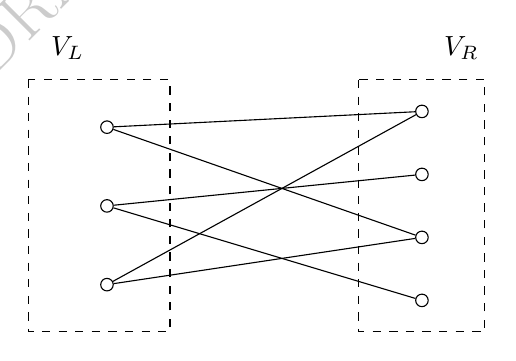
\begin{tikzpicture}[scale=1.0]
    \node at (-1.5,2.0) {$V_L$};
    \node at (3.5,2.0) {$V_R$};

    \node[circle,draw,inner sep=1.6pt] (a) at (-1,1) {};
    \node[circle,draw,inner sep=1.6pt] (b) at (-1,0) {};
    \node[circle,draw,inner sep=1.6pt] (c) at (-1,-1) {};

    \node[circle,draw,inner sep=1.6pt] (d) at (3,1.2) {};
    \node[circle,draw,inner sep=1.6pt] (e) at (3,0.4) {};
    \node[circle,draw,inner sep=1.6pt] (f) at (3,-0.4) {};
    \node[circle,draw,inner sep=1.6pt] (g) at (3,-1.2) {};

    \draw (a)--(d);
    \draw (a)--(f);
    \draw (b)--(e);
    \draw (b)--(g);
    \draw (c)--(d);
    \draw (c)--(f);

    \draw[dashed] (-2,1.6) rectangle (-0.2,-1.6);
    \draw[dashed] (2.2,1.6) rectangle (3.8,-1.6);
\end{tikzpicture}
\end{center}

\begin{theorem}{Bipartite graphs and \(2\)-colorability}{bipartite-two-colorable}
A graph \(G\) is bipartite if and only if
\[
\chi(G)\le 2.
\]
\end{theorem}

\begin{proof}
Suppose \(G\) is bipartite with bipartition
\[
V=V_L\sqcup V_R.
\]
Color all vertices in \(V_L\) with color \(1\), and all vertices in \(V_R\) with color \(2\). Since every edge goes between the two parts, this is a valid \(2\)-coloring. Hence \(\chi(G)\le 2\).

Conversely, suppose \(\chi(G)\le 2\). If \(G\) has a \(1\)-coloring, then \(G\) has no edges and is bipartite. If \(G\) has a \(2\)-coloring, let \(V_L\) be the set of vertices of color \(1\), and \(V_R\) the set of vertices of color \(2\). Adjacent vertices have different colors, so every edge goes between \(V_L\) and \(V_R\). Hence \(G\) is bipartite.
\end{proof}

\begin{theorem}{Odd-cycle characterization of bipartite graphs}{bipartite-odd-cycle}
A graph is bipartite if and only if it contains no odd cycle as a subgraph.
\end{theorem}

\begin{proof}
If \(G\) is bipartite, every cycle must alternate between the two parts \(V_L\) and \(V_R\). Returning to the starting vertex is possible only after an even number of steps. Hence every cycle in a bipartite graph has even length.

Conversely, if \(G\) has no odd cycle, one may color each connected component by choosing a starting vertex, coloring vertices at even distance from it with one color and vertices at odd distance from it with another. The absence of odd cycles ensures this is well-defined and produces a valid bipartition.
\end{proof}

\begin{examplebox}[title={Tutorial 9, Question 3}]
For \(K_n\), the graph is bipartite exactly when
\[
n=1\quad\text{or}\quad n=2.
\]
Indeed, \(K_n\) contains a triangle whenever \(n\ge 3\), and a triangle is an odd cycle.

For \(C_n\),
\[
C_n\text{ is bipartite}
\quad\Longleftrightarrow\quad
n\text{ is even}.
\]
This follows directly from the odd-cycle characterization.
\end{examplebox}

\begin{examtip}[title={Fast tests for bipartiteness}]
To prove a graph is bipartite, exhibit a bipartition or a \(2\)-coloring.

To prove it is not bipartite, find an odd cycle.
\end{examtip}

%==================================================
\subsection{Complete Bipartite Graphs}
%==================================================

\begin{definition}{Complete bipartite graph}{complete-bipartite}
The \emph{complete bipartite graph} \(K_{m,n}\) has vertex set
\[
V=V_1\sqcup V_2,
\qquad |V_1|=m,\quad |V_2|=n,
\]
with no edges inside \(V_1\) or inside \(V_2\), and with every vertex of \(V_1\) adjacent to every vertex of \(V_2\).
\end{definition}

\begin{keyformula}[title={Basic data for \(K_{m,n}\)}]
\[
|V(K_{m,n})|=m+n,
\qquad
|E(K_{m,n})|=mn.
\]
Each vertex in the \(m\)-part has degree \(n\), and each vertex in the \(n\)-part has degree \(m\).
\end{keyformula}

% Complete bipartite graph K_{3,3}.
\begin{center}
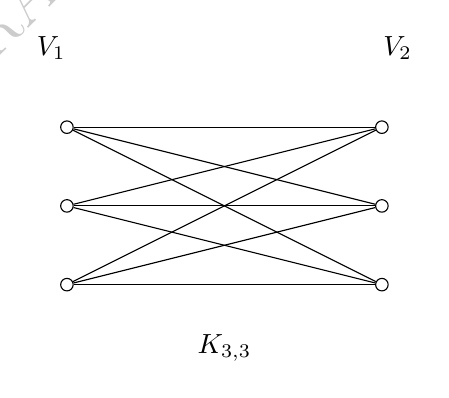
\begin{tikzpicture}[scale=1.0]
    \node at (-1.2,2.0) {$V_1$};
    \node at (3.2,2.0) {$V_2$};

    \foreach \i/\y in {1/1,2/0,3/-1}{
        \node[circle,draw,inner sep=1.6pt] (L\i) at (-1,\y) {};
    }
    \foreach \i/\y in {1/1,2/0,3/-1}{
        \node[circle,draw,inner sep=1.6pt] (R\i) at (3,\y) {};
    }

    \foreach \i in {1,2,3}{
        \foreach \j in {1,2,3}{
            \draw (L\i)--(R\j);
        }
    }

    \node at (1,-1.8) {$K_{3,3}$};
\end{tikzpicture}
\end{center}

\begin{examplebox}[title={Tutorial 9, Question 4}]
The degree sequence of \(K_{2,3}\) is
\[
3,3,2,2,2.
\]
For \(K_{m,n}\), the \(m\) vertices on one side each have degree \(n\), while the \(n\) vertices on the other side each have degree \(m\). Thus, if \(m\le n\), the degree sequence is
\[
\underbrace{n,n,\dots,n}_{m\text{ terms}},
\underbrace{m,m,\dots,m}_{n\text{ terms}}.
\]
\end{examplebox}

\begin{extension}[title={Adjacency-matrix viewpoint}]
If the vertices are ordered by the two parts of \(K_{m,n}\), then its adjacency matrix has block form
\[
\begin{pmatrix}
0 & J_{m\times n}\\
J_{n\times m} & 0
\end{pmatrix},
\]
where \(J\) is an all-ones matrix. Row sums immediately give the degree sequence.
\end{extension}

%==================================================
\subsection{Planar Graphs}
%==================================================

\begin{definition}{Planar graph and planar representation}{planar-graph}
A graph is \emph{planar} if it can be drawn in the plane so that no two edges cross except possibly at common endpoints.

A drawing with no such crossings is called a \emph{planar representation} of the graph.
\end{definition}

Planarity is a property of the abstract graph, not of one particular drawing. A graph may look non-planar in one drawing but still be planar if a different crossing-free drawing exists.

\begin{examplebox}[title={\(K_4\) is planar}]
The graph \(K_4\) may be drawn with crossings if all four vertices are placed on a square and both diagonals are drawn. However, it has a planar representation by placing one vertex inside a triangle and joining it to the three triangle vertices. Hence \(K_4\) is planar.
\end{examplebox}

% Planar drawing of K4 with one vertex inside a triangle.
\begin{center}
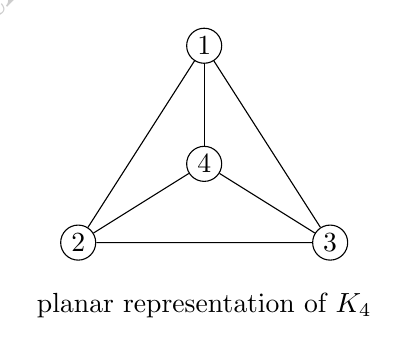
\begin{tikzpicture}[scale=1.0]
    \node[circle,draw,inner sep=1.6pt] (a) at (0,1.5) {$1$};
    \node[circle,draw,inner sep=1.6pt] (b) at (-1.6,-1) {$2$};
    \node[circle,draw,inner sep=1.6pt] (c) at (1.6,-1) {$3$};
    \node[circle,draw,inner sep=1.6pt] (d) at (0,0) {$4$};

    \draw (a)--(b)--(c)--(a);
    \draw (d)--(a);
    \draw (d)--(b);
    \draw (d)--(c);

    \node at (0,-1.8) {planar representation of \(K_4\)};
\end{tikzpicture}
\end{center}

\begin{commonmistake}[title={A non-planar-looking drawing is not a proof}]
To prove that a graph is non-planar, it is not enough to show one drawing with crossings. One must prove that \emph{no} crossing-free drawing exists.
\end{commonmistake}

%==================================================
\subsection{Regions and Euler's Formula}
%==================================================

\begin{definition}{Region / face}{region-face}
A planar representation of a graph divides the plane into \emph{regions}, also called \emph{faces}. One of these is the unbounded outside region, called the \emph{infinite region}.
\end{definition}

\begin{definition}{Degree of a region}{region-degree}
The \emph{degree} of a region \(R\), denoted \(\deg(R)\), is the number of edge-boundary occurrences around \(R\). If an edge appears twice on the boundary of a region, it contributes twice to \(\deg(R)\).
\end{definition}

% Planar graph with three regions labelled.
\begin{center}
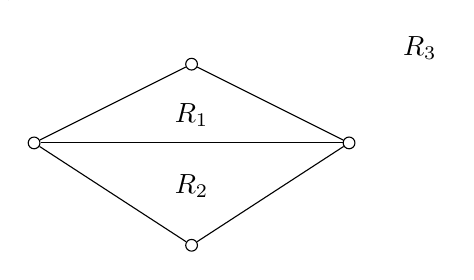
\begin{tikzpicture}[scale=1.0]
    \node[circle,draw,inner sep=1.5pt] (a) at (0,0) {};
    \node[circle,draw,inner sep=1.5pt] (b) at (2,1) {};
    \node[circle,draw,inner sep=1.5pt] (c) at (4,0) {};
    \node[circle,draw,inner sep=1.5pt] (d) at (2,-1.3) {};

    \draw (a)--(b)--(c)--(d)--(a);
    \draw (a)--(c);

    \node at (2,0.35) {\(R_1\)};
    \node at (2,-0.55) {\(R_2\)};
    \node at (4.9,1.2) {\(R_3\)};
\end{tikzpicture}
\end{center}

\begin{theorem}{Euler's Formula}{euler-formula}
Let \(G\) be a connected planar simple graph with
\[
n=|V|,\qquad m=|E|,
\]
and let \(r\) be the number of regions in a planar representation of \(G\). Then
\[
n-m+r=2.
\]
Equivalently,
\[
r=m-n+2.
\]
\end{theorem}

\begin{keyformula}[title={Euler's Formula}]
\[
n-m+r=2
\qquad
\text{for connected planar simple graphs.}
\]
\end{keyformula}

\begin{theorem}{Sum of the degrees of regions}{region-degree-sum}
In a planar representation of a planar graph,
\[
\sum_R \deg(R)=2m,
\]
where the sum is over all regions.
\end{theorem}

\begin{proof}
Every edge borders regions on its two sides. If the same region lies on both sides of an edge, that edge is counted twice in that region's boundary. Hence every edge contributes exactly \(2\) to the total sum of region degrees, so
\[
\sum_R\deg(R)=2m.
\]
\end{proof}

\begin{extension}[title={Dual handshaking idea}]
The identity
\[
\sum_R\deg(R)=2m
\]
is the face-version of the Handshaking Lemma. The usual Handshaking Lemma sums degrees over vertices; this one sums boundary degrees over regions.
\end{extension}

%==================================================
\subsection{Edge Bounds for Planar Graphs}
%==================================================

\begin{theorem}{Planar edge bound}{planar-edge-bound}
If \(G\) is a connected planar simple graph with \(n\ge 3\) vertices and \(m\) edges, then
\[
m\le 3n-6.
\]
\end{theorem}

\begin{proof}
Every region has degree at least \(3\), so
\[
2m=\sum_R\deg(R)\ge 3r.
\]
Hence
\[
r\le \frac{2m}{3}.
\]
Using Euler's formula,
\[
2=n-m+r\le n-m+\frac{2m}{3}=n-\frac{m}{3}.
\]
Thus
\[
m\le 3n-6.
\]
\end{proof}

\begin{theorem}{Triangle-free planar edge bound}{triangle-free-planar-bound}
If \(G\) is a connected simple planar graph with \(n\ge 3\) vertices, \(m\) edges, and no cycles of length \(3\), then
\[
m\le 2n-4.
\]
\end{theorem}

\begin{proof}
Since \(G\) has no \(3\)-cycles, every region has boundary degree at least \(4\). Thus
\[
2m=\sum_R\deg(R)\ge 4r,
\]
so
\[
r\le \frac{m}{2}.
\]
Euler's formula gives
\[
2=n-m+r\le n-m+\frac{m}{2}=n-\frac{m}{2}.
\]
Therefore
\[
m\le 2n-4.
\]
\end{proof}

\begin{keyformula}[title={Fast planar non-planarity tests}]
For simple planar graphs:
\[
m\le 3n-6
\qquad (n\ge 3).
\]
If there are no triangles:
\[
m\le 2n-4.
\]
Violating either relevant bound proves non-planarity.
\end{keyformula}

\begin{commonmistake}[title={These inequalities are one-way tests}]
If a graph violates the planar edge bound, it is non-planar. But satisfying the bound does \emph{not} guarantee planarity.
\end{commonmistake}

%==================================================
\subsection{Non-Planarity of \(K_5\) and \(K_{3,3}\)}
%==================================================

\begin{examplebox}[title={Non-planarity of \(K_5\)}]
The complete graph \(K_5\) has
\[
n=5,\qquad m=\binom{5}{2}=10.
\]
If \(K_5\) were planar, then the planar edge bound would give
\[
m\le 3n-6=3(5)-6=9.
\]
But
\[
10\le 9
\]
is false. Hence
\[
\boxed{K_5\text{ is not planar}.}
\]
\end{examplebox}

\begin{examplebox}[title={Non-planarity of \(K_{3,3}\)}]
The complete bipartite graph \(K_{3,3}\) has
\[
n=6,\qquad m=9.
\]
It has no triangles because it is bipartite. If it were planar, the triangle-free planar bound would give
\[
m\le 2n-4=2(6)-4=8.
\]
But
\[
9\le 8
\]
is false. Therefore
\[
\boxed{K_{3,3}\text{ is not planar}.}
\]
\end{examplebox}

\begin{examplebox}[title={Tutorial 9, Question 5}]
Removing one edge from \(K_{3,3}\) gives a graph with
\[
n=6,\qquad m=8.
\]
This no longer violates the triangle-free planar bound
\[
m\le 2n-4=8.
\]
Indeed, \(K_{3,3}\) with one edge removed has a planar drawing.

Similarly, removing one edge from \(K_5\) gives
\[
n=5,\qquad m=9,
\]
which no longer violates
\[
m\le 3n-6=9.
\]
Indeed, \(K_5\) with one edge removed is planar.
\end{examplebox}

\begin{examtip}[title={Choosing the right edge bound}]
Use
\[
m\le 3n-6
\]
for general simple planar graphs.

Use
\[
m\le 2n-4
\]
when the graph has no triangles, especially for bipartite graphs such as \(K_{3,3}\).
\end{examtip}

%==================================================
\subsection{Disconnected Planar Graphs}
%==================================================

The edge-count corollaries are often applied componentwise or by adding edges between components.

\begin{theorem}{Planar edge bounds for disconnected simple graphs}{disconnected-planar-bounds}
Let \(G\) be a simple planar graph with \(n\ge 3\) vertices and \(m\) edges. Then
\[
m\le 3n-6.
\]
If \(G\) has no cycles of length \(3\), then
\[
m\le 2n-4.
\]
\end{theorem}

\begin{proof}
If \(G\) is disconnected, add edges between connected components in a planar drawing until the graph becomes connected. This does not destroy planarity. The resulting connected planar graph has at least \(m\) edges and the same \(n\) vertices. Applying the connected case gives the same upper bound for the original graph.
\end{proof}

\begin{extension}[title={Why adding edges can help prove an upper bound}]
Adding edges to connect components can only increase the edge count. If the larger connected planar graph must satisfy an upper bound, then the original disconnected graph also satisfies it.
\end{extension}

%==================================================
\subsection{Homeomorphic Graphs and Kuratowski's Theorem}
%==================================================

\begin{definition}{Elementary subdivision}{elementary-subdivision}
An \emph{elementary subdivision} of an edge \(\{u,v\}\) removes the edge \(\{u,v\}\), adds a new vertex \(w\), and inserts the two edges
\[
\{u,w\},\qquad \{w,v\}.
\]
\end{definition}

\begin{definition}{Homeomorphic graphs}{homeomorphic-graphs}
Two graphs are \emph{homeomorphic} if they can be obtained from the same graph by a sequence of elementary subdivisions.
\end{definition}

% Elementary subdivision of an edge.
\begin{center}
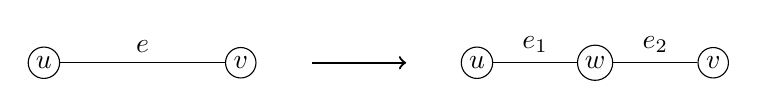
\begin{tikzpicture}[scale=1.0]
    \node[circle,draw,inner sep=1.5pt] (u1) at (0,0) {\(u\)};
    \node[circle,draw,inner sep=1.5pt] (v1) at (2.5,0) {\(v\)};
    \draw (u1)--node[above]{\(e\)}(v1);

    \draw[->,thick] (3.4,0)--(4.6,0);

    \node[circle,draw,inner sep=1.5pt] (u2) at (5.5,0) {\(u\)};
    \node[circle,draw,inner sep=1.5pt] (w) at (7.0,0) {\(w\)};
    \node[circle,draw,inner sep=1.5pt] (v2) at (8.5,0) {\(v\)};
    \draw (u2)--node[above]{\(e_1\)}(w)--node[above]{\(e_2\)}(v2);
\end{tikzpicture}
\end{center}

\begin{theorem}{Kuratowski's Theorem}{kuratowski}
A graph is non-planar if and only if it contains a subgraph homeomorphic to either
\[
K_5
\qquad\text{or}\qquad
K_{3,3}.
\]
\end{theorem}

\begin{extension}[title={How to interpret Kuratowski's Theorem}]
Kuratowski's Theorem says that \(K_5\) and \(K_{3,3}\) are the two fundamental obstructions to planarity, up to subdivision. In practice, the theorem is useful for recognizing hidden non-planar structure inside a larger graph.
\end{extension}

%==================================================
\subsection{Map Coloring and the Four-Color Theorem}
%==================================================

Map coloring can be converted into graph coloring. Represent each region of a map by a vertex. Join two vertices by an edge if the corresponding regions share a boundary segment.

\begin{definition}{Map adjacency graph}{map-adjacency-graph}
Given a map divided into regions, its \emph{adjacency graph} has:
\begin{itemize}[leftmargin=*]
    \item one vertex for each region;
    \item an edge between two vertices if the corresponding regions share a common boundary segment.
\end{itemize}
Touching at only a corner does not count as adjacency.
\end{definition}

\begin{theorem}{Four-Color Theorem}{four-color-theorem}
Every simple planar graph is \(4\)-colorable.
\end{theorem}

\begin{keyformula}[title={Four-Color Theorem}]
\[
G\text{ simple and planar}
\quad\Longrightarrow\quad
\chi(G)\le 4.
\]
\end{keyformula}

\begin{examplebox}[title={Map coloring as graph coloring}]
To color a map, construct the region-adjacency graph. A valid coloring of the map is then exactly a valid vertex-coloring of this graph.
\end{examplebox}

\begin{commonmistake}[title={Four colors is an upper bound, not always the exact value}]
The Four-Color Theorem says
\[
\chi(G)\le 4
\]
for every simple planar graph \(G\). It does not say that every planar graph has chromatic number exactly \(4\). Many planar graphs are \(1\)-, \(2\)-, or \(3\)-colorable.
\end{commonmistake}

\begin{examplebox}[title={Tutorial 9, Question 6}]
A planar graph can have chromatic number \(4\). The standard example is
\[
K_4.
\]
It is planar, and since every pair of vertices is adjacent,
\[
\chi(K_4)=4.
\]
Thus \(K_4\) shows that the Four-Color Theorem is sharp.
\end{examplebox}

%==================================================
\subsection{Special Techniques}
%==================================================

\subsubsection*{1. Prove colorability by constructing a coloring}
To show \(\chi(G)\le k\), explicitly give a \(k\)-coloring or describe a coloring algorithm.

\subsubsection*{2. Prove lower bounds by finding cliques or odd cycles}
If \(G\) contains a copy of \(K_t\), then
\[
\chi(G)\ge t.
\]
If \(G\) contains an odd cycle, then
\[
\chi(G)\ge 3.
\]

\subsubsection*{3. Prove bipartiteness using a bipartition}
For a positive result, explicitly write
\[
V=V_L\sqcup V_R
\]
and check that every edge crosses between the parts.

\subsubsection*{4. Disprove bipartiteness using an odd cycle}
A single odd cycle is enough to prove that a graph is not bipartite.

\subsubsection*{5. Prove planarity by drawing}
To prove a graph is planar, it is enough to provide one crossing-free planar representation.

\subsubsection*{6. Prove non-planarity using edge bounds}
For simple graphs, first test:
\[
m\le 3n-6.
\]
For triangle-free graphs, especially bipartite graphs, test:
\[
m\le 2n-4.
\]

\subsubsection*{7. Use Kuratowski's Theorem for hidden obstructions}
If the edge-count inequalities do not prove non-planarity, search for a subdivision of \(K_5\) or \(K_{3,3}\).

\begin{extension}[title={Fast decision tree for Handout 09}]
\[
\begin{array}{c|c}
\text{Question type} & \text{Fast first move} \\ \hline
\text{Is the graph bipartite?} & \text{try a 2-coloring or find an odd cycle} \\
\text{Find }\chi(G) & \text{give upper coloring and lower obstruction} \\
\text{Is the graph planar?} & \text{try drawing it without crossings} \\
\text{Prove non-planarity} & \text{test edge bounds, then search for }K_5/K_{3,3}
\end{array}
\]
A complete solution often needs both an upper bound and a lower bound.
\end{extension}

%==================================================
\subsection{Summary Table}
%==================================================

\begin{center}
\small
\begin{tabular}{@{}p{0.28\textwidth}p{0.30\textwidth}p{0.31\textwidth}@{}}
\toprule
\textbf{Concept} & \textbf{Definition / formula} & \textbf{Exam use} \\
\midrule
\(k\)-coloring & \(f:V\to\{1,\dots,k\}\), adjacent vertices different & prove colorability \\
Chromatic number & \(\chi(G)=\min k\) for valid \(k\)-coloring & exact color requirement \\
Bipartite graph & \(V=V_L\sqcup V_R\), all edges cross parts & equivalent to \(\chi(G)\le 2\) \\
Odd-cycle criterion & bipartite \(\Longleftrightarrow\) no odd cycle & fast non-bipartite test \\
Complete bipartite graph & \(K_{m,n}\), all cross edges present & \(|E|=mn\) \\
Planar graph & drawable without crossings & one drawing proves planarity \\
Euler's formula & \(n-m+r=2\) & connected planar graphs \\
Region degree sum & \(\sum_R\deg(R)=2m\) & derive edge bounds \\
Planar edge bound & \(m\le 3n-6\) & fast non-planarity test \\
Triangle-free bound & \(m\le 2n-4\) & useful for bipartite graphs \\
Kuratowski obstruction & contains subdivision of \(K_5\) or \(K_{3,3}\) & deeper non-planarity test \\
Four-Color Theorem & planar simple graph \(\Rightarrow \chi(G)\le 4\) & map coloring upper bound \\
\bottomrule
\end{tabular}
\end{center}

\begin{examtip}[title={Final checklist for Handout 09}]
Before finalizing a solution, check:
\begin{enumerate}[leftmargin=*]
    \item If proving colorability, did you give a valid coloring?
    \item If proving a chromatic number exactly, did you prove both upper and lower bounds?
    \item If proving bipartiteness, did you give a bipartition or use the odd-cycle criterion?
    \item If proving planarity, did you provide a crossing-free drawing?
    \item If proving non-planarity, did you use a valid obstruction rather than relying on a bad drawing?
\end{enumerate}
\end{examtip}

\begin{commonmistake}[title={Final warning for Handout 09}]
A drawing with crossing edges proves nothing by itself. Planarity is about whether \emph{some} crossing-free drawing exists. Conversely, coloring a graph with too many colors gives only a weak upper bound; to find \(\chi(G)\), one must also prove that fewer colors are impossible.
\end{commonmistake}
}{}
\IfFileExists{chapters/handout10.tex}{\input{chapters/handout10.tex}}{}
\IfFileExists{chapters/handout11.tex}{% Source reference: :contentReference[oaicite:0]{index=0}
\part{Graph Theory}
\section{Handout 11: Graph Theory (5): Minimum Spanning Trees, Shortest Paths}

\subsection{Overview}

This handout is the final graph-theory handout. It focuses on two weighted-graph optimisation problems:
\begin{itemize}[leftmargin=*]
    \item \emph{minimum spanning tree} problems: connect all vertices with minimum total edge weight;
    \item \emph{shortest path} problems: find minimum-weight routes between vertices.
\end{itemize}

The main algorithms are:
\[
\text{Kruskal's Algorithm},
\qquad
\text{Prim's Algorithm},
\qquad
\text{Dijkstra's Algorithm}.
\]

The central distinction is:
\[
\text{MST: choose edges to connect all vertices}
\qquad\text{versus}\qquad
\text{Shortest path: choose a route between vertices}.
\]

\begin{examtip}[title={Main diagnostic for Handout 11}]
Before applying an algorithm, identify the objective:
\[
\begin{array}{c|c}
\text{Objective} & \text{Relevant method} \\ \hline
\text{connect all vertices with minimum total weight} & \text{MST: Kruskal / Prim} \\
\text{shortest route from one source to one target} & \text{Dijkstra until target settled} \\
\text{shortest routes from one source to all vertices} & \text{full Dijkstra}
\end{array}
\]
Do not use MST algorithms to solve shortest-path problems, and do not use shortest-path algorithms to build MSTs.
\end{examtip}

%==================================================
\subsection{Algorithms}
%==================================================

\begin{definition}{Algorithm}{algorithm-def}
An \emph{algorithm} is a finite mechanical procedure that starts with an input and produces an output after executing a sequence of well-defined primitive steps.
\end{definition}

Two basic criteria for judging an algorithm are:
\begin{itemize}[leftmargin=*]
    \item \emph{correctness}: the algorithm always returns the desired output;
    \item \emph{running time}: the number of primitive steps needed as a function of input size.
\end{itemize}

\begin{examtip}[title={How algorithms are assessed in this handout}]
The lecture emphasises correctness ideas more than detailed complexity analysis. For MST algorithms, correctness is based on safe edges and cut arguments. For Dijkstra's algorithm, correctness is based on settling vertices in increasing distance from the source.
\end{examtip}

%==================================================
\subsection{Recall: Spanning Trees and Minimum Spanning Trees}
%==================================================

\begin{definition}{Spanning tree}{spanning-tree-recall}
Let \(G=(V,E)\) be a connected simple graph. A \emph{spanning tree} of \(G\) is a subgraph \(T\) of \(G\) such that:
\begin{itemize}[leftmargin=*]
    \item \(T\) is a tree;
    \item \(V(T)=V(G)\).
\end{itemize}
\end{definition}

\begin{definition}{Minimum spanning tree}{mst-def}
Let \(G=(V,E,W)\) be a connected edge-weighted graph, where
\[
W:E\to \mathbb{R}
\]
assigns a weight or cost to each edge. A \emph{minimum spanning tree}, abbreviated MST, is a spanning tree \(T\) of \(G\) whose total weight
\[
W(T)=\sum_{e\in E(T)}W(e)
\]
is as small as possible among all spanning trees of \(G\).
\end{definition}

\begin{keyformula}[title={MST objective}]
\[
\text{minimize }
\sum_{e\in E(T)}W(e)
\qquad
\text{over all spanning trees }T\text{ of }G.
\]
\end{keyformula}

\begin{examplebox}[title={What an MST must satisfy}]
If \(G\) is connected and has \(n\) vertices, then every MST:
\begin{itemize}[leftmargin=*]
    \item contains all \(n\) vertices;
    \item has exactly \(n-1\) edges;
    \item is connected;
    \item contains no cycle;
    \item has minimum total weight among all spanning trees.
\end{itemize}
\end{examplebox}

\begin{commonmistake}[title={MST is not usually a shortest-path tree}]
A minimum spanning tree minimizes the \emph{total} weight needed to connect all vertices. It does not necessarily preserve the shortest path from a chosen source to every other vertex.
\end{commonmistake}

%==================================================
\subsection{Greedy Approach to MST}
%==================================================

Both Kruskal's and Prim's algorithms are greedy algorithms. At each step, they make a locally cheapest choice that is guaranteed to be safe.

A generic MST greedy algorithm has the form:
\[
\begin{array}{l}
T\leftarrow \varnothing;\\
\text{while }T\text{ is not a spanning tree:}\\
\qquad \text{choose an edge }e\text{ satisfying a safe condition};\\
\qquad T\leftarrow T\cup\{e\};\\
\text{return }T.
\end{array}
\]

The key mathematical question is:

\begin{center}
\emph{Which locally cheap edges are guaranteed to belong to an MST?}
\end{center}

This is answered by the cut property.

\begin{examtip}[title={Greedy algorithms need proof}]
A greedy choice is not correct merely because it is cheap. The proof must show that the chosen edge can safely belong to an MST.
\end{examtip}

%==================================================
\subsection{Cuts and Safe Edges}
%==================================================

\begin{definition}{Cut}{cut-def}
Let \(G=(V,E)\) be a graph. A \emph{cut} is a partition of \(V\) into two disjoint nonempty subsets
\[
S
\qquad\text{and}\qquad
V\setminus S.
\]
An edge \(\{u,v\}\in E\) \emph{crosses the cut} if one endpoint lies in \(S\) and the other lies in \(V\setminus S\).
\end{definition}

% Cut diagram showing vertices split into S and V\S with crossing edges.
\begin{center}
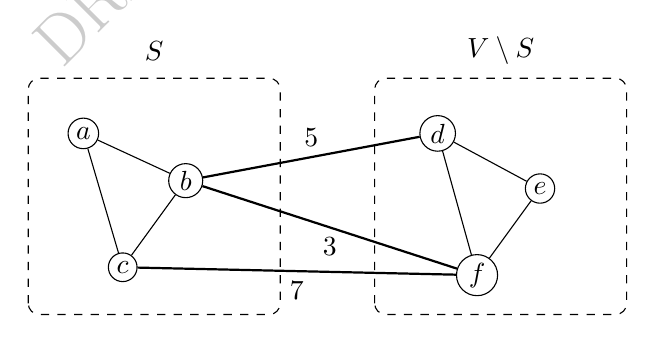
\begin{tikzpicture}[scale=1.0]
    \draw[dashed,rounded corners] (-1.2,-1.5) rectangle (2.0,1.5);
    \draw[dashed,rounded corners] (3.2,-1.5) rectangle (6.4,1.5);
    \node at (0.4,1.85) {\(S\)};
    \node at (4.8,1.85) {\(V\setminus S\)};

    \node[circle,draw,inner sep=1.5pt] (a) at (-0.5,0.8) {\(a\)};
    \node[circle,draw,inner sep=1.5pt] (b) at (0.8,0.2) {\(b\)};
    \node[circle,draw,inner sep=1.5pt] (c) at (0.0,-0.9) {\(c\)};

    \node[circle,draw,inner sep=1.5pt] (d) at (4.0,0.8) {\(d\)};
    \node[circle,draw,inner sep=1.5pt] (e) at (5.3,0.1) {\(e\)};
    \node[circle,draw,inner sep=1.5pt] (f) at (4.5,-1.0) {\(f\)};

    \draw (a)--(b)--(c)--(a);
    \draw (d)--(e)--(f)--(d);
    \draw[thick] (b)--node[above]{\(5\)}(d);
    \draw[thick] (b)--node[below]{\(3\)}(f);
    \draw[thick] (c)--node[below]{\(7\)}(f);
\end{tikzpicture}
\end{center}

\begin{definition}{Safe edge}{safe-edge}
Assume the edge costs in a connected undirected graph are distinct. An edge \(e\) is called a \emph{safe edge} if there exists a cut
\[
(S,V\setminus S)
\]
such that \(e\) is the unique minimum-cost edge crossing that cut.
\end{definition}

\begin{theorem}{Cut property}{cut-property}
Assume \(G\) is a connected undirected graph with distinct edge costs. Then every safe edge belongs to every minimum spanning tree of \(G\).
\end{theorem}

\begin{proof}
Let \(e=\{u,v\}\) be safe for the cut \((S,V\setminus S)\), and suppose for contradiction that some MST \(T\) does not contain \(e\).

Adding \(e\) to \(T\) creates a unique cycle. Since \(e\) crosses the cut, the cycle must contain another edge \(e'\) that also crosses the same cut. Because \(e\) is the unique minimum-cost edge crossing the cut,
\[
W(e)<W(e').
\]
Now replace \(e'\) by \(e\):
\[
T'=(T\setminus\{e'\})\cup\{e\}.
\]
The graph \(T'\) is still a spanning tree, but
\[
W(T')=W(T)-W(e')+W(e)<W(T),
\]
contradicting that \(T\) is an MST. Therefore every MST contains \(e\).
\end{proof}

\begin{theorem}{Safe edges form the unique MST under distinct costs}{safe-edges-mst}
Assume \(G\) is connected and all edge costs are distinct. Then the set of all safe edges forms the unique minimum spanning tree of \(G\).
\end{theorem}

\begin{proof}
By the cut property, every safe edge belongs to every MST.

It remains to see that the safe edges connect all vertices. Suppose the graph formed by the safe edges is not connected. Let \(S\) be the vertex set of one of its connected components. Since \(G\) is connected, at least one edge of \(G\) crosses the cut \((S,V\setminus S)\). Because edge costs are distinct, there is a unique minimum-cost edge crossing this cut. By definition, that edge is safe, but then it would connect \(S\) to \(V\setminus S\), contradicting that \(S\) was a component of the safe-edge graph.

Hence the safe edges form a connected spanning subgraph. Since every safe edge belongs to every MST and an MST has exactly \(n-1\) edges, these safe edges are exactly the unique MST.
\end{proof}

\begin{extension}[title={Why distinct costs simplify the theory}]
Distinct edge costs ensure that each cut has a unique cheapest crossing edge. Without distinct costs, MSTs may not be unique, but Kruskal's and Prim's algorithms still produce an MST when ties are handled arbitrarily.
\end{extension}

%==================================================
\subsection{Kruskal's Algorithm}
%==================================================

Kruskal's algorithm grows a forest. It processes edges globally from cheapest to most expensive and adds an edge exactly when it does not create a cycle.

\begin{theorem}{Kruskal's Algorithm}{kruskal-algorithm}
Given a connected undirected edge-weighted graph \(G=(V,E,W)\):
\[
\begin{array}{l}
T\leftarrow \varnothing;\\
\text{sort edges in increasing order of weight;}\\
\text{for each edge }e\text{ in this order:}\\
\qquad \text{if }T\cup\{e\}\text{ contains no cycle, then }T\leftarrow T\cup\{e\};\\
\qquad \text{stop once }|T|=|V|-1;\\
\text{return }T.
\end{array}
\]
The returned graph \(T\) is a minimum spanning tree.
\end{theorem}

\begin{proof}
At every stage, \(T\) is a forest. Suppose Kruskal adds an edge \(e=\{u,v\}\). Let \(S\) be the vertex set of the connected component of \(T\) containing \(u\) just before \(e\) is added. Since \(e\) does not form a cycle, \(v\notin S\), so \(e\) crosses the cut \((S,V\setminus S)\).

Any cheaper edge crossing this cut would also connect two different components at the time it was considered, and hence would have been added earlier. Therefore \(e\) is the cheapest edge crossing this cut. Under distinct costs, it is the unique cheapest crossing edge, so it is safe.

Thus every edge added by Kruskal is safe and hence belongs to the MST. The algorithm stops after adding \(n-1\) edges without forming a cycle, so the result is a spanning tree. Since all its edges are safe, it is the MST.
\end{proof}

\begin{keyformula}[title={Kruskal's rule}]
\[
\text{Process edges by increasing weight; add the next edge iff it does not create a cycle.}
\]
\end{keyformula}

\begin{examplebox}[title={Kruskal example}]
Let \(G\) have vertices
\[
\{a,b,c,d,e\}
\]
and weighted edges
\[
ab:1,\quad bc:2,\quad ac:3,\quad bd:4,\quad cd:5,\quad de:6,\quad ce:7.
\]
Process edges in increasing order:
\[
ab,\ bc,\ ac,\ bd,\ cd,\ de,\ ce.
\]
Kruskal adds:
\[
ab,\quad bc,
\]
then skips \(ac\) because \(ab,bc,ac\) would form a cycle. It then adds
\[
bd,\quad de.
\]
Now there are \(5-1=4\) edges, so the algorithm stops. The MST is
\[
\{ab,bc,bd,de\}
\]
with total weight
\[
1+2+4+6=13.
\]
\end{examplebox}

\begin{commonmistake}[title={Kruskal is not ``choose the cheapest adjacent edge''}]
Kruskal does not grow one connected tree from a starting vertex. It may maintain several components at once. Its only rule is global increasing edge order plus the no-cycle test.
\end{commonmistake}

%==================================================
\subsection{Prim's Algorithm}
%==================================================

Prim's algorithm grows one tree. It starts from a vertex and repeatedly attaches the cheapest edge from the current tree to a new vertex.

\begin{theorem}{Prim's Algorithm}{prim-algorithm}
Given a connected undirected edge-weighted graph \(G=(V,E,W)\), choose a starting vertex \(s\). Then:
\[
\begin{array}{l}
T\leftarrow \varnothing;\\
S\leftarrow \{s\};\\
\text{while }S\neq V:\\
\qquad \text{choose a minimum-weight edge }e=\{u,v\}\\
\qquad \text{with }u\in S\text{ and }v\in V\setminus S;\\
\qquad T\leftarrow T\cup\{e\};\\
\qquad S\leftarrow S\cup\{v\};\\
\text{return }T.
\end{array}
\]
The returned graph \(T\) is a minimum spanning tree.
\end{theorem}

\begin{proof}
At each step, \(S\) is the vertex set of the tree currently built by the algorithm. The edge chosen by Prim is the minimum-weight edge crossing the cut
\[
(S,V\setminus S).
\]
Under distinct costs, it is the unique minimum crossing edge, so it is safe by the cut property. Therefore every edge added belongs to the MST.

Each iteration adds exactly one new vertex to \(S\), so the algorithm eventually reaches \(S=V\). The selected edges connect all vertices and contain no cycle because each new edge attaches one new vertex. Hence the output is a spanning tree made of safe edges, and therefore is the MST.
\end{proof}

\begin{keyformula}[title={Prim's rule}]
\[
\text{Grow one tree; repeatedly add the cheapest edge crossing from the tree to outside.}
\]
\end{keyformula}

\begin{examplebox}[title={Prim example on the same graph}]
Using the graph from the Kruskal example and starting at \(a\):
\[
ab:1,\quad bc:2,\quad ac:3,\quad bd:4,\quad cd:5,\quad de:6,\quad ce:7.
\]
Start with
\[
S=\{a\}.
\]
The cheapest edge leaving \(S\) is \(ab\), so add \(b\):
\[
S=\{a,b\}.
\]
The cheapest edge leaving \(S\) is \(bc\), so add \(c\):
\[
S=\{a,b,c\}.
\]
The cheapest edge leaving \(S\) is \(bd\), so add \(d\):
\[
S=\{a,b,c,d\}.
\]
Finally the cheapest edge leaving \(S\) is \(de\), so add \(e\). The MST is again
\[
\{ab,bc,bd,de\},
\]
with total weight \(13\).
\end{examplebox}

\begin{examtip}[title={Kruskal versus Prim}]
\[
\begin{array}{c|c}
\text{Kruskal} & \text{global edge order; avoids cycles} \\
\text{Prim} & \text{one growing tree; crosses the current cut}
\end{array}
\]
Both rely on the same cut-property idea.
\end{examtip}

%==================================================
\subsection{Shortest Paths in Weighted Graphs}
%==================================================

\begin{definition}{Weighted graph and path length}{weighted-path}
Let \(G=(V,E,W)\) be an edge-weighted graph. If an edge \(e=(u,v)\) has weight
\[
\ell(e)=\ell(u,v),
\]
then the \emph{length} of a path is the sum of the weights of all edges on the path.
\end{definition}

\begin{definition}{Shortest path and distance}{shortest-path-distance}
Let \(u,v\in V\). A \emph{shortest path} from \(u\) to \(v\) is a simple path from \(u\) to \(v\) whose total length is minimum among all paths from \(u\) to \(v\).

The \emph{distance} from \(u\) to \(v\), denoted \(d(u,v)\), is the length of a shortest path from \(u\) to \(v\). If no path connects \(u\) to \(v\), then
\[
d(u,v)=\infty.
\]
\end{definition}

In this handout, shortest-path algorithms are studied for graphs with \emph{non-negative} edge lengths.

\begin{examplebox}[title={Shortest path interpretation}]
If vertices represent MRT stations or road junctions, and edge weights represent travel time or distance, then a shortest path represents a route of minimum total travel cost.
\end{examplebox}

\begin{commonmistake}[title={Fewest edges need not mean shortest path}]
A path with fewer edges may have larger total weight than a path with more edges. Shortest path means minimum total edge weight, not minimum number of edges.
\end{commonmistake}

\subsubsection{Types of shortest-path problems}

Typical shortest-path problems include:
\begin{enumerate}[leftmargin=*]
    \item \emph{single-pair shortest path}: given \(s,t\), find a shortest path from \(s\) to \(t\);
    \item \emph{single-source shortest paths}: given \(s\), find shortest paths from \(s\) to all vertices;
    \item \emph{all-pairs shortest paths}: find shortest paths between all pairs of vertices.
\end{enumerate}

This handout focuses mainly on the first two. For undirected graphs, each undirected edge may be replaced by two directed edges of the same weight, one in each direction.

% Directed replacement of an undirected weighted edge.
\begin{center}
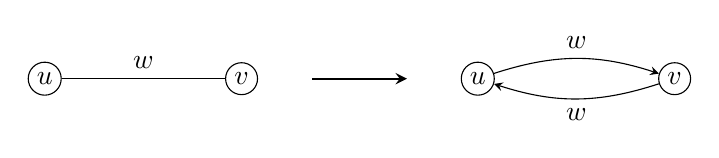
\begin{tikzpicture}[>=stealth,scale=1.0]
    \node[circle,draw,inner sep=1.7pt] (u1) at (0,0) {\(u\)};
    \node[circle,draw,inner sep=1.7pt] (v1) at (2.5,0) {\(v\)};
    \draw (u1)--node[above]{\(w\)}(v1);

    \draw[->,thick] (3.4,0)--(4.6,0);

    \node[circle,draw,inner sep=1.7pt] (u2) at (5.5,0) {\(u\)};
    \node[circle,draw,inner sep=1.7pt] (v2) at (8.0,0) {\(v\)};
    \draw[->,bend left=18] (u2) to node[above]{\(w\)} (v2);
    \draw[->,bend left=18] (v2) to node[below]{\(w\)} (u2);
\end{tikzpicture}
\end{center}

%==================================================
\subsection{Shortest Path Structure}
%==================================================

The correctness of Dijkstra's algorithm rests on two structural facts.

\begin{theorem}{Subpaths of shortest paths are shortest}{shortest-subpath}
Let
\[
s=v_0\to v_1\to\cdots\to v_k=v
\]
be a shortest path from \(s\) to \(v\). Then for every \(1\le i<k\), the subpath
\[
s=v_0\to v_1\to\cdots\to v_i
\]
is a shortest path from \(s\) to \(v_i\).
\end{theorem}

\begin{proof}
Suppose the subpath from \(s\) to \(v_i\) were not shortest. Then there would be another path from \(s\) to \(v_i\) with smaller total length. Replacing the original initial segment by this shorter path would produce a path from \(s\) to \(v\) shorter than the original path, contradicting that the original path was shortest.
\end{proof}

\begin{theorem}{Next closest vertex principle}{next-closest}
Suppose \(S\) contains the already-settled vertices closest to a source \(s\). If \(u\notin S\) is the next closest vertex to \(s\), then a shortest path from \(s\) to \(u\) reaches \(u\) by one final edge from some vertex in \(S\).
\end{theorem}

\begin{proof}
Let
\[
P:s=v_0\to v_1\to\cdots\to v_k=u
\]
be a shortest path from \(s\) to \(u\). Every intermediate vertex \(v_i\), with \(i<k\), has distance
\[
d(s,v_i)<d(s,u)
\]
when edge lengths are non-negative and the path is simple. Therefore each such intermediate vertex is already among the closer settled vertices in \(S\). In particular, the predecessor \(v_{k-1}\) of \(u\) lies in \(S\), and the last step is an edge from \(S\) to \(u\).
\end{proof}

\begin{extension}[title={Why non-negative weights matter}]
Dijkstra's algorithm relies on the fact that extending a path cannot reduce its length. Negative edge weights can invalidate the claim that once a vertex is chosen as closest, its distance is final.
\end{extension}

%==================================================
\subsection{Tentative Distances and Relaxation}
%==================================================

Let \(s\) be the source vertex. For each vertex \(v\), Dijkstra's algorithm maintains a tentative distance \(d(v)\).

\begin{definition}{Relaxation}{relaxation}
Given a directed edge \((u,v)\) with length \(\ell(u,v)\), \emph{relaxing} the edge means replacing
\[
d(v)
\]
by
\[
\min\{d(v),\,d(u)+\ell(u,v)\}.
\]
\end{definition}

The idea is that if the best known path to \(u\) has length \(d(u)\), then travelling from \(u\) to \(v\) gives a candidate path to \(v\) of length
\[
d(u)+\ell(u,v).
\]

\begin{keyformula}[title={Relaxation update}]
\[
d(v)\leftarrow \min\{d(v),\,d(u)+\ell(u,v)\}.
\]
\end{keyformula}

% Relaxation diagram showing a candidate improvement from u to v.
\begin{center}
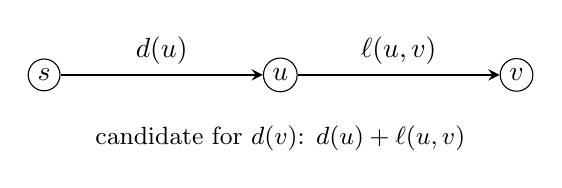
\begin{tikzpicture}[>=stealth,scale=1.0]
    \node[circle,draw,inner sep=1.8pt] (s) at (0,0) {\(s\)};
    \node[circle,draw,inner sep=1.8pt] (u) at (3,0) {\(u\)};
    \node[circle,draw,inner sep=1.8pt] (v) at (6,0) {\(v\)};

    \draw[->,thick] (s)--node[above]{\(d(u)\)}(u);
    \draw[->,thick] (u)--node[above]{\(\ell(u,v)\)}(v);

    \node at (3,-0.8) {\small candidate for \(d(v)\): \(d(u)+\ell(u,v)\)};
\end{tikzpicture}
\end{center}

\begin{examtip}[title={Relaxation is the atomic step of Dijkstra}]
Every update in Dijkstra's algorithm is a relaxation of an outgoing edge from the newly settled vertex.
\end{examtip}

%==================================================
\subsection{Dijkstra's Algorithm}
%==================================================

\begin{theorem}{Dijkstra's Algorithm}{dijkstra-algorithm}
Let \(G=(V,E)\) be a directed weighted graph with non-negative edge lengths, and let \(s\in V\). Dijkstra's algorithm computes the shortest-path distance from \(s\) to every vertex reachable from \(s\):
\[
\begin{array}{l}
\text{for every }v\in V,\ d(v)\leftarrow \infty;\\
d(s)\leftarrow 0;\\
S\leftarrow \varnothing;\\[0.2em]
\text{while }S\neq V:\\
\qquad \text{choose }u\in V\setminus S\text{ with minimum }d(u);\\
\qquad S\leftarrow S\cup\{u\};\\
\qquad \text{for each edge }(u,v)\text{ with }v\notin S:\\
\qquad\qquad d(v)\leftarrow \min\{d(v),d(u)+\ell(u,v)\};\\
\text{return the values }d(v).
\end{array}
\]
\end{theorem}

\begin{proof}
We prove by induction on the number of iterations that whenever a vertex \(u\) is added to \(S\), the value \(d(u)\) equals the true shortest distance from \(s\) to \(u\).

Initially, \(d(s)=0\), and no other vertex can have distance less than \(0\) because edge lengths are non-negative.

Assume the claim holds for all vertices already in \(S\). Let \(u\in V\setminus S\) be chosen with minimum tentative distance. Suppose, for contradiction, that there is a shorter path \(P\) from \(s\) to \(u\) than \(d(u)\). Along \(P\), let \(y\) be the first vertex not in \(S\), and let \(x\) be the vertex immediately before \(y\). Then \(x\in S\).

By the induction hypothesis, \(d(x)\) is already the true shortest distance to \(x\). When \(x\) was added to \(S\), the edge \((x,y)\) was relaxed, so
\[
d(y)\le d(x)+\ell(x,y).
\]
The portion of \(P\) from \(s\) to \(y\) is no longer than the full path \(P\) from \(s\) to \(u\), because edge lengths are non-negative. Thus \(d(y)\) is less than the alleged shorter length to \(u\), and hence less than \(d(u)\). But \(u\) was chosen as the vertex outside \(S\) with minimum tentative distance, a contradiction.

Therefore \(d(u)\) is final when \(u\) is added to \(S\). By induction, the algorithm is correct.
\end{proof}

\begin{keyformula}[title={Dijkstra invariant}]
Once a vertex enters \(S\), its tentative value \(d(v)\) is final:
\[
v\in S
\quad\Longrightarrow\quad
d(v)=\text{true shortest distance from }s\text{ to }v.
\]
\end{keyformula}

\begin{commonmistake}[title={Dijkstra is not valid for negative edge lengths}]
The correctness proof uses non-negative edge lengths. If negative edges are allowed, a vertex that appears settled may later be improved through a negative edge.
\end{commonmistake}

%==================================================
\subsection{Worked Dijkstra Example}
%==================================================

Consider the directed weighted graph with vertices
\[
\{a,b,c,d,e,z\}
\]
and directed edges
\[
a\to b:4,\quad a\to c:2,\quad c\to b:1,\quad c\to d:8,\quad c\to e:10,
\]
\[
b\to d:5,\quad d\to e:2,\quad d\to z:6,\quad e\to z:3.
\]

% Directed weighted graph for Dijkstra example.
\begin{center}
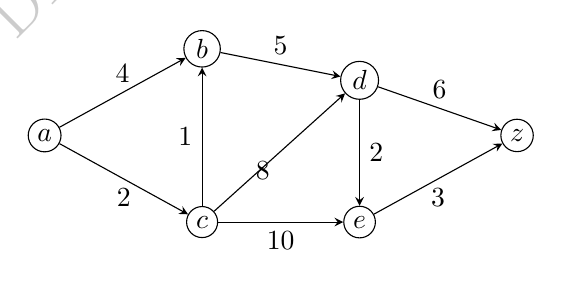
\begin{tikzpicture}[>=stealth,scale=1.0]
    \node[circle,draw,inner sep=1.8pt] (a) at (0,0) {\(a\)};
    \node[circle,draw,inner sep=1.8pt] (c) at (2,-1.1) {\(c\)};
    \node[circle,draw,inner sep=1.8pt] (b) at (2,1.1) {\(b\)};
    \node[circle,draw,inner sep=1.8pt] (d) at (4,0.7) {\(d\)};
    \node[circle,draw,inner sep=1.8pt] (e) at (4,-1.1) {\(e\)};
    \node[circle,draw,inner sep=1.8pt] (z) at (6,0) {\(z\)};

    \draw[->] (a)--node[above]{\(4\)}(b);
    \draw[->] (a)--node[below]{\(2\)}(c);
    \draw[->] (c)--node[left]{\(1\)}(b);
    \draw[->] (b)--node[above]{\(5\)}(d);
    \draw[->] (c)--node[below left]{\(8\)}(d);
    \draw[->] (c)--node[below]{\(10\)}(e);
    \draw[->] (d)--node[right]{\(2\)}(e);
    \draw[->] (d)--node[above]{\(6\)}(z);
    \draw[->] (e)--node[below]{\(3\)}(z);
\end{tikzpicture}
\end{center}

\begin{examplebox}[title={Dijkstra from source \(a\)}]
Initialize
\[
d(a)=0,\qquad d(b)=d(c)=d(d)=d(e)=d(z)=\infty,
\qquad S=\varnothing.
\]

The successive table of tentative distances is:
\[
\begin{array}{c|cccccc|c}
\text{Round} & d(a)&d(b)&d(c)&d(d)&d(e)&d(z)&S\\ \hline
0 &0&\infty&\infty&\infty&\infty&\infty&\varnothing\\
1 &0&4&2&\infty&\infty&\infty&\{a\}\\
2 &0&3&2&10&12&\infty&\{a,c\}\\
3 &0&3&2&8&12&\infty&\{a,c,b\}\\
4 &0&3&2&8&10&14&\{a,c,b,d\}\\
5 &0&3&2&8&10&13&\{a,c,b,d,e\}\\
6 &0&3&2&8&10&13&\{a,c,b,d,e,z\}.
\end{array}
\]

Thus the final shortest-path distances from \(a\) are:
\[
d(a)=0,\quad d(c)=2,\quad d(b)=3,\quad d(d)=8,\quad d(e)=10,\quad d(z)=13.
\]
\end{examplebox}

\begin{extension}[title={Recovering actual shortest paths}]
To recover the shortest path itself, not just its length, store a predecessor each time a relaxation improves \(d(v)\). For example, if \(d(v)\) is improved using \(u\to v\), set
\[
\operatorname{pred}(v)=u.
\]
Tracing predecessors backward from the target reconstructs the shortest path.
\end{extension}

%==================================================
\subsection{Shortest Path Algorithm with \(\pi\)-Values}
%==================================================

The handout first presents Dijkstra's idea using values
\[
\pi(u)=\min_{a\in S}\{d(a)+\ell(a,u)\}
\]
for unexplored vertices \(u\notin S\). Here \(S\) is the set of vertices whose shortest distances have already been determined.

\begin{theorem}{\(\pi\)-value selection rule}{pi-selection-rule}
Assume \(S\) contains the already settled vertices. For \(u\in V\setminus S\), define
\[
\pi(u)=\min_{a\in S}\{d(a)+\ell(a,u)\}.
\]
Then the next closest vertex to \(s\) is a vertex \(u\in V\setminus S\) minimizing \(\pi(u)\).
\end{theorem}

\begin{proof}
By the next closest vertex principle, a shortest path to the next closest unsettled vertex enters it from some settled vertex \(a\in S\). Thus its distance is of the form
\[
d(a)+\ell(a,u)
\]
for some \(a\in S\), and the best such value is \(\pi(u)\). Therefore the next closest vertex is obtained by minimizing \(\pi(u)\) over all vertices outside \(S\).
\end{proof}

The efficient implementation stores these \(\pi\)-values directly as the tentative distances \(d(v)\). When a new vertex \(u\) is settled, only edges leaving \(u\) need to be scanned.

\begin{examtip}[title={Why the optimized update is enough}]
Since \(S\) only grows, the only new possible shortest route to an unsettled vertex \(v\) after adding \(u\) is a route that enters \(v\) through \(u\). Hence the update
\[
d(v)\leftarrow \min\{d(v),d(u)+\ell(u,v)\}
\]
is sufficient.
\end{examtip}

%==================================================
\subsection{MST versus Shortest Path Trees}
%==================================================

Both MST and shortest-path algorithms output trees in many situations, but the objectives are different.

\begin{center}
\small
\begin{tabular}{@{}p{0.24\textwidth}p{0.31\textwidth}p{0.33\textwidth}@{}}
\toprule
\textbf{Object} & \textbf{Objective} & \textbf{Typical algorithm} \\
\midrule
Minimum spanning tree & minimize total cost of connecting all vertices & Kruskal / Prim \\
Shortest path tree from \(s\) & minimize distance from \(s\) to each vertex & Dijkstra \\
\bottomrule
\end{tabular}
\end{center}

\begin{examplebox}[title={Different objectives can give different trees}]
A spanning tree of small total weight may give a long route between two particular vertices. Conversely, the union of shortest paths from a source may have larger total weight than an MST. Therefore the two problems should be treated separately.
\end{examplebox}

%==================================================
\subsection{Special Techniques}
%==================================================

\subsubsection*{1. Use cut arguments for MST correctness}
To prove an edge is safe, find a cut for which that edge is the unique cheapest crossing edge.

\subsubsection*{2. For Kruskal, track components}
Kruskal's algorithm is easiest to execute by maintaining connected components. Add an edge exactly when its endpoints lie in different components.

\subsubsection*{3. For Prim, track the growing vertex set}
Prim's algorithm is easiest to execute by maintaining the current vertex set \(S\). Add the cheapest edge crossing from \(S\) to \(V\setminus S\).

\subsubsection*{4. For Dijkstra, maintain settled and unsettled vertices}
The settled set \(S\) contains vertices whose shortest distances are final. Always choose the unsettled vertex with smallest tentative distance.

\subsubsection*{5. Relax outgoing edges systematically}
After settling \(u\), update every outgoing neighbour \(v\) using
\[
d(v)\leftarrow \min\{d(v),d(u)+\ell(u,v)\}.
\]

\subsubsection*{6. Stop early for a single target}
If the goal is only to find a shortest path from \(s\) to \(t\), Dijkstra can stop once \(t\) is added to \(S\).

\subsubsection*{7. Check assumptions before using an algorithm}
For MST algorithms, the graph should be connected and undirected. For Dijkstra in this handout, edge lengths must be non-negative.

\begin{extension}[title={Unified greedy viewpoint}]
Kruskal, Prim, and Dijkstra are all greedy, but their invariants differ:
\[
\begin{array}{c|c}
\text{Algorithm} & \text{Invariant} \\ \hline
\text{Kruskal} & T\text{ is a forest of safe edges} \\
\text{Prim} & T\text{ is one tree of safe edges} \\
\text{Dijkstra} & S\text{ contains vertices with finalized shortest distances}
\end{array}
\]
Remembering the invariant prevents mixing the algorithms.
\end{extension}

%==================================================
\subsection{Summary Table}
%==================================================

\begin{center}
\small
\begin{tabular}{@{}p{0.25\textwidth}p{0.31\textwidth}p{0.33\textwidth}@{}}
\toprule
\textbf{Concept} & \textbf{Definition / rule} & \textbf{Exam use} \\
\midrule
Spanning tree & tree subgraph containing all vertices & connects graph minimally by edges \\
MST & spanning tree of minimum total weight & optimal network design \\
Cut & partition \((S,V\setminus S)\) & isolates crossing edges \\
Safe edge & unique minimum edge crossing some cut & belongs to every MST under distinct costs \\
Cut property & safe edges are in every MST & correctness of MST algorithms \\
Kruskal & add edges in increasing weight if no cycle forms & MST by global edge order \\
Prim & repeatedly add cheapest edge crossing current cut & MST by growing one tree \\
Path length & sum of edge weights on a path & weighted route cost \\
Distance & length of a shortest path, or \(\infty\) if unreachable & shortest-path value \\
Relaxation & \(d(v)\leftarrow\min\{d(v),d(u)+\ell(u,v)\}\) & Dijkstra update step \\
Dijkstra & settle vertices in increasing tentative distance & single-source shortest paths \\
\bottomrule
\end{tabular}
\end{center}

\begin{examtip}[title={Final checklist for Handout 11}]
Before finalizing a solution, check:
\begin{enumerate}[leftmargin=*]
    \item Is the problem asking for an MST or a shortest path?
    \item For an MST problem, have you avoided cycles while connecting all vertices?
    \item For Kruskal, did you process edges in increasing order?
    \item For Prim, did you choose the cheapest edge crossing from the current tree?
    \item For Dijkstra, are all edge weights non-negative?
    \item After each Dijkstra step, did you relax outgoing edges from the newly settled vertex?
    \item If a vertex remains at distance \(\infty\), is it unreachable from the source?
\end{enumerate}
\end{examtip}

\begin{commonmistake}[title={Final warning for Handout 11}]
Kruskal, Prim, and Dijkstra are all greedy algorithms, but they solve different optimisation problems. Kruskal and Prim minimize total spanning-tree weight; Dijkstra minimizes distances from a source.
\end{commonmistake}}{}
\IfFileExists{chapters/handout12.tex}{% Source reference: :contentReference[oaicite:0]{index=0}
\part{Review}
\section{Handout 12: Review}

\subsection{Overview}

This handout is a final review of the whole MH1301 syllabus. It does not introduce a new mathematical topic; instead, it consolidates the three major parts of the module:
\[
\text{Counting},
\qquad
\text{Recurrence Relations},
\qquad
\text{Graph Theory}.
\]

The final-exam emphasis described in the handout is approximately:
\[
\begin{array}{c|c}
\text{Part} & \text{Approximate weight} \\ \hline
\text{Counting} & 35\% \\
\text{Recurrence Relations} & 30\% \\
\text{Graph Theory} & 35\%
\end{array}
\]
The question allocation is described as:
\[
\text{Questions 1--2: Counting},
\qquad
\text{Questions 3--4: Recurrence Relations},
\qquad
\text{Questions 5--6: Graph Theory}.
\]

\begin{examtip}[title={How to read this review chapter}]
This chapter should be used as a synthesis checklist, not as a replacement for the earlier handout chapters. For each item below, you should be able to:
\begin{enumerate}[leftmargin=*]
    \item state the relevant definition or theorem accurately;
    \item identify when it applies;
    \item solve at least one tutorial-style problem using it;
    \item explain one common mistake associated with it.
\end{enumerate}
\end{examtip}

%==================================================
\subsection{Final Exam Structure and Revision Priorities}
%==================================================

The final exam covers the full lecture syllabus except material explicitly marked optional. The structure is designed to contain a substantial number of accessible marks, together with more challenging questions that test problem-solving flexibility.

\begin{center}
\small
\begin{tabular}{@{}p{0.28\textwidth}p{0.26\textwidth}p{0.36\textwidth}@{}}
\toprule
\textbf{Question type} & \textbf{Approximate marks} & \textbf{Expected revision response} \\
\midrule
Easy questions & \(50\) marks & secure definitions, direct formulas, standard algorithms \\
Slightly more challenging questions & \(25\) marks & combine two or more ideas, handle cases carefully \\
Challenging questions & \(25\) marks & structural reasoning, proof, obstruction, non-routine modelling \\
\bottomrule
\end{tabular}
\end{center}

\begin{examtip}[title={Efficient exam-preparation order}]
A practical final-review order is:
\[
\begin{aligned}
\text{definitions}&\longrightarrow\text{standard formulas}
\longrightarrow\text{worked tutorial problems}\\
&\longrightarrow\text{mixed-topic practice}
\longrightarrow\text{one-page reference sheet}.
\end{aligned}
\]
Do not start by memorising formulas without first knowing which problem type each formula solves.
\end{examtip}

\begin{commonmistake}[title={Treating the reference sheet as a substitute for reasoning}]
A one-page reference sheet can remind you of formulas, but it cannot decide whether order matters, whether cases are disjoint, whether a recurrence is homogeneous, or whether a graph problem is Eulerian or Hamiltonian. Those decisions must be practised before the exam.
\end{commonmistake}

%==================================================
\subsection{Counting Review}
%==================================================

Counting questions require modelling discipline. Before applying a formula, decide what the objects are, whether order matters, whether repetition is allowed, and whether the cases overlap.

\subsubsection{Sum Rule, Product Rule, Division Rule, and Bijection}

\begin{theorem}{Sum Rule}{review-sum-rule}
If \(A_1,A_2,\dots,A_n\) are pairwise disjoint finite sets, then
\[
|A_1\cup A_2\cup\cdots\cup A_n|
=
|A_1|+|A_2|+\cdots+|A_n|.
\]
\end{theorem}

\begin{theorem}{Product Rule}{review-product-rule}
If an object is constructed in \(k\) successive stages, with \(n_i\) choices at stage \(i\), then the total number of objects is
\[
n_1n_2\cdots n_k.
\]
\end{theorem}

\begin{theorem}{Division Rule}{review-division-rule}
If every object in a target set is represented exactly \(k\) times by a larger counted set, then
\[
\text{target count}
=
\frac{\text{larger count}}{k}.
\]
\end{theorem}

\begin{theorem}{Bijection Principle}{review-bijection}
If \(f:X\to Y\) is a bijection between finite sets, then
\[
|X|=|Y|.
\]
\end{theorem}

\begin{examtip}[title={Which basic rule should be used?}]
\[
\begin{array}{c|c}
\text{Situation} & \text{Rule} \\ \hline
\text{disjoint cases} & \text{Sum Rule} \\
\text{sequential choices} & \text{Product Rule} \\
\text{uniform overcounting} & \text{Division Rule} \\
\text{hard objects encoded as easier objects} & \text{Bijection Principle}
\end{array}
\]
\end{examtip}

\begin{commonmistake}[title={Adding before checking disjointness}]
The Sum Rule applies only to disjoint cases. If an object can belong to two cases simultaneously, direct addition overcounts.
\end{commonmistake}

\subsubsection{Inclusion--Exclusion}

\begin{keyformula}[title={Inclusion--exclusion}]
For two sets,
\[
|A\cup B|=|A|+|B|-|A\cap B|.
\]
For three sets,
\[
|A\cup B\cup C|
=
|A|+|B|+|C|
-|A\cap B|-|A\cap C|-|B\cap C|
+|A\cap B\cap C|.
\]
In general,
\[
\left|\bigcup_{i=1}^{n}A_i\right|
=
\sum_i |A_i|
-
\sum_{i<j}|A_i\cap A_j|
+
\sum_{i<j<k}|A_i\cap A_j\cap A_k|
-\cdots .
\]
\end{keyformula}

\begin{examplebox}[title={Counting objects avoiding forbidden conditions}]
Suppose \(U\) is a universal set and \(A,B,C\) are three bad events. The number of objects avoiding all three bad events is
\[
|U\setminus(A\cup B\cup C)|
=
|U|-|A|-|B|-|C|
+|A\cap B|+|A\cap C|+|B\cap C|
-|A\cap B\cap C|.
\]
This form is especially useful for forbidden substrings, divisibility restrictions, and overlapping cases.
\end{examplebox}

\begin{extension}[title={Why the signs alternate}]
An object lying in exactly \(r\) of the sets is counted
\[
\binom{r}{1}-\binom{r}{2}+\binom{r}{3}-\cdots+(-1)^{r-1}\binom{r}{r}=1
\]
time in the inclusion--exclusion sum. Thus every object in the union contributes exactly once.
\end{extension}

\subsubsection{Pigeonhole Principle}

\begin{theorem}{Pigeonhole Principle}{review-php}
If \(N\) objects are placed into \(k\) boxes, then at least one box contains at least
\[
\left\lceil \frac{N}{k}\right\rceil
\]
objects.
\end{theorem}

\begin{examtip}[title={Pigeonhole modelling}]
A pigeonhole problem is solved by identifying:
\[
\text{objects}
\quad\text{and}\quad
\text{boxes/categories}.
\]
Common boxes include remainders modulo \(n\), first letters, parity classes, degree values, and possible values of a bounded quantity.
\end{examtip}

\subsubsection{Binomial Theorem and Combinatorial Proof}

\begin{theorem}{Binomial Theorem}{review-binomial}
For every nonnegative integer \(n\),
\[
(x+y)^n
=
\sum_{i=0}^{n}\binom{n}{i}x^{n-i}y^i.
\]
\end{theorem}

\begin{definition}{Combinatorial proof}{review-comb-proof}
A \emph{combinatorial proof} proves an identity by showing that both sides count the same family of objects in two different ways.
\end{definition}

\begin{examplebox}[title={Pascal identity by counting}]
To prove
\[
\binom{n+1}{r}=\binom{n}{r}+\binom{n}{r-1},
\]
count \(r\)-element subsets of an \((n+1)\)-element set. Fix one distinguished element \(x\). The subset either excludes \(x\), giving \(\binom{n}{r}\) choices, or includes \(x\), giving \(\binom{n}{r-1}\) choices.
\end{examplebox}

\subsubsection{Permutations and Combinations}

\begin{keyformula}[title={Core permutation and combination formulas}]
\[
P(n,r)=\frac{n!}{(n-r)!},
\qquad
C(n,r)=\binom{n}{r}=\frac{n!}{r!(n-r)!}.
\]
\[
\text{ordered with repetition: }n^r,
\qquad
\text{unordered with repetition: }\binom{n+r-1}{r}.
\]
\[
\text{indistinguishable objects: }
\frac{n!}{n_1!n_2!\cdots n_k!},
\qquad
\text{around a cycle: }
\frac{P(n,r)}{r}.
\]
\end{keyformula}

\begin{center}
\small
\begin{tabular}{@{}p{0.30\textwidth}p{0.27\textwidth}p{0.27\textwidth}@{}}
\toprule
& \textbf{\(r\)-permutation} & \textbf{\(r\)-combination} \\
\midrule
without repetition &
\[
P(n,r)=\frac{n!}{(n-r)!}
\]
&
\[
\binom{n}{r}=\frac{n!}{r!(n-r)!}
\]
\\[1em]
with repetition &
\[
n^r
\]
&
\[
\binom{n+r-1}{r}
\]
\\[1em]
with indistinguishable objects &
\[
\frac{n!}{n_1!n_2!\cdots n_k!}
\]
&
\[
\text{multiset / stars--bars model}
\]
\\[1em]
around a cycle &
\[
\frac{P(n,r)}{r}
\]
&
\[
\text{usually handled by symmetry}
\]
\\
\bottomrule
\end{tabular}
\end{center}

\begin{commonmistake}[title={The most common counting error}]
Do not choose a formula before deciding whether the selection is ordered or unordered. A committee is usually unordered; a ranking, password, string, or ordered seating is ordered.
\end{commonmistake}

%==================================================
\subsection{Recurrence Relations Review}
%==================================================

A recurrence question usually has one of two tasks:
\[
\text{derive the recurrence}
\qquad\text{or}\qquad
\text{solve the recurrence}.
\]
The correct solution starts by identifying which task is being asked.

\subsubsection{Setting Up Recurrences}

\begin{definition}{Recurrence relation}{review-recurrence}
A \emph{recurrence relation} for a sequence \((a_n)\) is a formula that expresses \(a_n\) in terms of earlier terms such as
\[
a_{n-1},a_{n-2},\dots,a_{n-k}.
\]
A recurrence model is incomplete unless the necessary initial values are specified.
\end{definition}

\begin{examtip}[title={Deriving a recurrence}]
To derive a recurrence:
\begin{enumerate}[leftmargin=*]
    \item define \(a_n\) precisely;
    \item identify the size parameter \(n\);
    \item split the size-\(n\) objects into disjoint cases;
    \item express each case using smaller values;
    \item state the initial values.
\end{enumerate}
\end{examtip}

\begin{examplebox}[title={Typical Fibonacci-type recurrence}]
Let \(a_n\) count binary strings of length \(n\) with no consecutive zeros. Split by the ending:
\begin{itemize}[leftmargin=*]
    \item strings ending in \(1\): \(a_{n-1}\) choices;
    \item strings ending in \(10\): \(a_{n-2}\) choices.
\end{itemize}
Thus
\[
a_n=a_{n-1}+a_{n-2},
\]
with suitable initial values such as \(a_1=2\), \(a_2=3\).
\end{examplebox}

\subsubsection{Linear Homogeneous Recurrences}

\begin{definition}{Linear homogeneous recurrence}{review-linear-hom}
A linear homogeneous recurrence relation of degree \(k\) with constant coefficients has the form
\[
a_n=c_1a_{n-1}+c_2a_{n-2}+\cdots+c_ka_{n-k},
\qquad c_k\neq 0.
\]
\end{definition}

\begin{keyformula}[title={Characteristic equation}]
For
\[
a_n=c_1a_{n-1}+c_2a_{n-2}+\cdots+c_ka_{n-k},
\]
the characteristic equation is
\[
r^k-c_1r^{k-1}-c_2r^{k-2}-\cdots-c_{k-1}r-c_k=0.
\]
\end{keyformula}

\begin{theorem}{Solution forms for homogeneous recurrences}{review-hom-solution}
For a linear homogeneous recurrence with constant coefficients:
\begin{itemize}[leftmargin=*]
    \item if the characteristic roots \(r_1,\dots,r_k\) are distinct, then
    \[
    a_n=h_1r_1^n+h_2r_2^n+\cdots+h_kr_k^n;
    \]
    \item if \(r\) is a repeated root of multiplicity \(m\), then its contribution is
    \[
    (h_0+h_1n+\cdots+h_{m-1}n^{m-1})r^n.
    \]
\end{itemize}
\end{theorem}

\begin{examplebox}[title={Distinct-root example}]
Solve
\[
a_n=5a_{n-1}-6a_{n-2}.
\]
The characteristic equation is
\[
r^2-5r+6=0=(r-2)(r-3),
\]
so the general solution is
\[
a_n=h_1\,2^n+h_2\,3^n.
\]
Initial values determine \(h_1,h_2\).
\end{examplebox}

\begin{examplebox}[title={Repeated-root example}]
Solve
\[
a_n=6a_{n-1}-9a_{n-2}.
\]
The characteristic equation is
\[
r^2-6r+9=0=(r-3)^2.
\]
Thus
\[
a_n=(h_1+h_2n)3^n.
\]
\end{examplebox}

\subsubsection{Linear Non-Homogeneous Recurrences}

\begin{definition}{Linear non-homogeneous recurrence}{review-nonhom}
A linear non-homogeneous recurrence relation has the form
\[
a_n=c_1a_{n-1}+\cdots+c_ka_{n-k}+F(n),
\]
where \(F(n)\) is a forcing term depending on \(n\).
\end{definition}

\begin{theorem}{Structure of non-homogeneous solutions}{review-nonhom-structure}
If \(a_n^{(p)}\) is one particular solution of a non-homogeneous recurrence and \(b_n\) is the general solution of the associated homogeneous recurrence, then the general solution is
\[
a_n=a_n^{(p)}+b_n.
\]
\end{theorem}

\begin{keyformula}[title={Particular-solution trial forms}]
\[
\begin{array}{c|c|c}
\text{Forcing term }F(n) & \text{No resonance} & \text{Resonance} \\ \hline
\text{polynomial of degree }t & \text{degree-}t\text{ polynomial} &
n\times\text{degree-}t\text{ polynomial} \\
s^n & c\,s^n & c\,n\,s^n
\end{array}
\]
For polynomial forcing, resonance means \(1\) is a characteristic root.
For exponential forcing \(s^n\), resonance means \(s\) is a characteristic root.
\end{keyformula}

\begin{commonmistake}[title={Using initial conditions too early}]
For non-homogeneous recurrences, first find the full form
\[
a_n=a_n^{(p)}+b_n.
\]
Only after that should the initial conditions be used to determine the constants.
\end{commonmistake}

%==================================================
\subsection{Graph Theory Review}
%==================================================

Graph theory questions usually test precise definitions, theorem triggers, and structural reasoning. The first step is to identify which class of graph problem is being asked:
\[
\text{degree / isomorphism},
\quad
\text{traversal},
\quad
\text{coloring / planarity},
\quad
\text{trees / algorithms}.
\]

\subsubsection{Basic Graph Language}

\begin{definition}{Graph terminology}{review-graph-terminology}
A graph \(G=(V,E)\) consists of a vertex set \(V\) and an edge set \(E\). Key terms include:
\begin{itemize}[leftmargin=*]
    \item adjacent vertices and incident edges;
    \item degree \(\deg(v)\);
    \item directed and undirected graphs;
    \item simple graphs;
    \item subgraphs and induced subgraphs;
    \item paths, circuits, connected components, and edge-weighted graphs.
\end{itemize}
\end{definition}

\begin{theorem}{Handshaking Lemma}{review-handshaking}
For an undirected graph,
\[
\sum_{v\in V}\deg(v)=2|E|.
\]
For a directed graph,
\[
\sum_{v\in V}\deg^-(v)=\sum_{v\in V}\deg^+(v)=|E|.
\]
\end{theorem}

\begin{examtip}[title={Fast graph invariant checks}]
To disprove isomorphism quickly, compare:
\[
\begin{aligned}
&|V|,\quad |E|,\quad \text{degree sequence},\\
&\text{number of isolated vertices},\quad
\text{adjacency patterns among equal-degree vertices}.
\end{aligned}
\]
If any invariant differs, the graphs are not isomorphic.
\end{examtip}

\begin{keyformula}[title={Special graph data}]
\[
|E(K_n)|=\binom{n}{2},
\qquad
\deg_{K_n}(v)=n-1.
\]
\[
|V(K_{m,n})|=m+n,
\qquad
|E(K_{m,n})|=mn.
\]
\[
C_n\text{ has }n\text{ vertices, }n\text{ edges, and every vertex has degree }2.
\]
\end{keyformula}

\subsubsection{Euler and Hamilton Traversals}

\begin{definition}{Euler and Hamilton objects}{review-euler-hamilton}
An \emph{Euler path/circuit} uses every edge exactly once.

A \emph{Hamilton path/circuit} visits every vertex exactly once, with the starting vertex repeated at the end for a Hamilton circuit.
\end{definition}

\begin{keyformula}[title={Euler criteria for connected graphs}]
For a connected graph:
\[
\begin{array}{c|c}
\text{number of odd-degree vertices} & \text{Euler conclusion} \\ \hline
0 & \text{Euler circuit exists} \\
2 & \text{Euler path exists, but no Euler circuit} \\
\text{otherwise} & \text{no Euler path}
\end{array}
\]
\end{keyformula}

\begin{commonmistake}[title={Euler versus Hamilton}]
Euler problems are about using \emph{edges}. Hamilton problems are about visiting \emph{vertices}. Euler has simple degree tests in this course; Hamilton usually requires construction or obstruction.
\end{commonmistake}

\subsubsection{Coloring and Bipartite Graphs}

\begin{definition}{Chromatic number and bipartite graph}{review-coloring-bipartite}
A \(k\)-coloring assigns colors to vertices so that adjacent vertices receive different colors. The chromatic number \(\chi(G)\) is the smallest valid number of colors.

A graph is \emph{bipartite} if its vertex set can be partitioned into two parts so that every edge crosses between the two parts.
\end{definition}

\begin{theorem}{Bipartite characterization}{review-bipartite}
A graph is bipartite if and only if it contains no odd cycle. Equivalently,
\[
G\text{ bipartite}
\quad\Longleftrightarrow\quad
\chi(G)\le 2.
\]
\end{theorem}

\begin{examplebox}[title={Standard chromatic numbers}]
\[
\chi(K_n)=n,
\qquad
\chi(C_n)=
\begin{cases}
2, & n\text{ even},\\
3, & n\text{ odd}.
\end{cases}
\]
\end{examplebox}

\subsubsection{Planar Graphs}

\begin{definition}{Planar graph}{review-planar}
A graph is \emph{planar} if it can be drawn in the plane with no crossings between edges except at common endpoints.
\end{definition}

\begin{theorem}{Euler's Formula for connected planar graphs}{review-euler-formula}
If \(G\) is a connected planar simple graph with \(n\) vertices, \(m\) edges, and \(r\) regions, then
\[
n-m+r=2.
\]
Equivalently,
\[
r=m-n+2.
\]
\end{theorem}

\begin{keyformula}[title={Planar edge bounds}]
For a simple planar graph with \(n\ge 3\),
\[
m\le 3n-6.
\]
If the graph has no \(3\)-cycles, then
\[
m\le 2n-4.
\]
In particular,
\[
K_5\text{ and }K_{3,3}\text{ are non-planar}.
\]
\end{keyformula}

\begin{theorem}{Four-Color Theorem}{review-four-color}
Every simple planar graph is \(4\)-colorable:
\[
G\text{ simple and planar}
\quad\Longrightarrow\quad
\chi(G)\le 4.
\]
\end{theorem}

\begin{commonmistake}[title={Bad drawing is not non-planarity}]
A drawing with crossings does not prove non-planarity. To prove non-planarity, use an obstruction such as an edge-count bound, \(K_5\), \(K_{3,3}\), or a subdivision of one of them.
\end{commonmistake}

\subsubsection{Trees and Spanning Trees}

\begin{definition}{Tree and spanning tree}{review-tree-spanning}
A \emph{tree} is a connected graph with no cycles. A \emph{forest} is a graph whose connected components are trees.

A \emph{spanning tree} of a connected graph \(G\) is a tree subgraph containing every vertex of \(G\).
\end{definition}

\begin{keyformula}[title={Tree formulas and rooted-tree terminology}]
If \(T\) is a tree with \(n\) vertices and \(m\) edges, then
\[
m=n-1.
\]
A binary tree of height \(h\) has at most
\[
2^h
\]
leaves.
Rooted-tree terminology includes root, parent, child, ancestor, descendant, level, height, and subtree.
\end{keyformula}

\begin{examtip}[title={Tree recognition}]
Common tree tests:
\[
\text{connected and acyclic},
\qquad
\text{connected and }m=n-1,
\qquad
\text{acyclic and }m=n-1.
\]
Use the version matching the information given in the question.
\end{examtip}

\subsubsection{Minimum Spanning Trees and Shortest Paths}

\begin{definition}{Minimum spanning tree and shortest path}{review-mst-sp}
A \emph{minimum spanning tree} is a spanning tree with minimum total edge weight.

A \emph{shortest path} between two vertices in a weighted graph is a path of minimum total edge length.
\end{definition}

\begin{keyformula}[title={Kruskal, Prim, and Dijkstra}]
\[
\begin{array}{c|p{0.62\textwidth}}
\text{Algorithm} & \text{Core rule} \\ \hline
\text{Kruskal} & process edges by increasing weight; add an edge if it creates no cycle \\
\text{Prim} & grow one tree; repeatedly add the cheapest edge from the current tree to a new vertex \\
\text{Dijkstra} & repeatedly settle the unsettled vertex with smallest tentative distance and relax its outgoing edges
\end{array}
\]
For Dijkstra,
\[
d(v)\leftarrow \min\{d(v),\,d(u)+\ell(u,v)\}.
\]
\end{keyformula}

\begin{commonmistake}[title={MST versus shortest path}]
Kruskal and Prim minimize total weight needed to connect all vertices. Dijkstra minimizes distances from a chosen source. These are different objectives and generally produce different trees.
\end{commonmistake}

%==================================================
\subsection{Reference-Sheet Planning}
%==================================================

The exam permits one double-sided A4 reference sheet. A good reference sheet should be organised by problem type, not merely by lecture order.

\begin{examtip}[title={Suggested reference-sheet layout}]
A high-value reference sheet may be organised as:
\[
\begin{array}{c|p{0.60\textwidth}}
\text{Block} & \text{Contents} \\ \hline
\text{Counting} & inclusion--exclusion, permutation/combination table, stars--bars, pigeonhole, binomial theorem \\
\text{Recurrences} & characteristic equation, distinct/repeated root forms, non-homogeneous trial forms \\
\text{Graph basics} & Handshaking Lemma, graph invariants, special graph data \\
\text{Traversals} & Euler criteria, Hamilton distinction \\
\text{Coloring/planarity} & bipartite tests, Euler's formula, planar edge bounds, Four-Color Theorem \\
\text{Trees/algorithms} & tree tests, MST algorithms, Dijkstra update rule
\end{array}
\]
\end{examtip}

\begin{commonmistake}[title={Reference sheet too formula-heavy}]
A useful reference sheet should include theorem triggers and common traps, not just formulas. For example, next to
\[
m\le 3n-6
\]
write ``simple planar, \(n\ge3\), one-way non-planarity test''.
\end{commonmistake}

%==================================================
\subsection{Integrated Exam Strategy}
%==================================================

\subsubsection{Questions 1--2: Counting}

For counting questions, first classify the object:
\[
\text{string},\quad
\text{subset},\quad
\text{function},\quad
\text{arrangement},\quad
\text{distribution},\quad
\text{cycle},\quad
\text{object avoiding bad events}.
\]
Then select the method.

\begin{examtip}[title={Counting solution template}]
A polished counting solution usually has the form:
\begin{enumerate}[leftmargin=*]
    \item define the set being counted;
    \item split into cases or build in stages;
    \item justify disjointness or correct overlap;
    \item apply the relevant formula;
    \item simplify only after the structure is correct.
\end{enumerate}
\end{examtip}

\subsubsection{Questions 3--4: Recurrences}

For recurrence questions, decide whether the question asks for modelling or solving.

\begin{examtip}[title={Recurrence solution template}]
For a solving question:
\begin{enumerate}[leftmargin=*]
    \item identify homogeneous or non-homogeneous type;
    \item write the characteristic equation of the associated homogeneous recurrence;
    \item write the general homogeneous solution;
    \item find a particular solution if needed;
    \item impose initial conditions.
\end{enumerate}
For a modelling question, define the state and derive the recurrence by disjoint cases.
\end{examtip}

\subsubsection{Questions 5--6: Graph Theory}

Graph theory questions should be handled by exact definitions first.

\begin{examtip}[title={Graph-theory solution template}]
A polished graph-theory solution usually begins by identifying the theorem class:
\[
\text{degree count},
\quad
\text{connectivity},
\quad
\text{Euler/Hamilton},
\quad
\text{coloring},
\quad
\text{planarity},
\quad
\text{tree},
\quad
\text{algorithm}.
\]
Then apply the relevant theorem with all hypotheses checked.
\end{examtip}

\begin{extension}[title={How to handle challenging questions}]
The challenging questions are likely to require a structural observation rather than a long calculation. Typical useful moves include:
\begin{itemize}[leftmargin=*]
    \item count the same object in two ways;
    \item use a complement or forbidden-event formulation;
    \item reduce a recurrence to a known form;
    \item use a graph invariant to disprove isomorphism;
    \item use a parity or edge-count obstruction;
    \item construct an explicit coloring, path, tree, or algorithm trace.
\end{itemize}
\end{extension}

%==================================================
\subsection{Special Techniques}
%==================================================

\subsubsection*{1. Classify before calculating}
Most MH1301 problems are solved by choosing the correct model. Decide whether the task is counting, recurrence modelling, recurrence solving, or graph-structure analysis before applying formulas.

\subsubsection*{2. Use disjoint partitions}
Whenever the phrase ``either/or'' appears in a counting or recurrence problem, verify that the cases are disjoint. If not, refine the partition or apply inclusion--exclusion.

\subsubsection*{3. Convert objects into strings, subsets, functions, or equations}
Many counting problems become standard after recoding:
\[
\text{subsets}\leftrightarrow\text{binary strings},
\qquad
\text{multisets}\leftrightarrow\text{stars and bars},
\qquad
\text{assignments}\leftrightarrow\text{functions}.
\]

\subsubsection*{4. Use characteristic equations only for the right recurrence class}
The characteristic-equation method applies to linear recurrences with constant coefficients. If the recurrence is non-homogeneous, first solve the associated homogeneous recurrence and then add a particular solution.

\subsubsection*{5. Match graph problems to theorem triggers}
Use:
\[
\begin{array}{c|c}
\text{Clue} & \text{Likely theorem} \\ \hline
\text{degrees and edges} & \text{Handshaking Lemma} \\
\text{use every edge} & \text{Euler criteria} \\
\text{visit every vertex} & \text{Hamilton construction/obstruction} \\
\text{two-coloring} & \text{bipartite / odd-cycle test} \\
\text{no crossings} & \text{planarity / Euler formula} \\
\text{connected and acyclic} & \text{tree theory} \\
\text{minimum connection cost} & \text{MST algorithms} \\
\text{minimum route from source} & \text{Dijkstra}
\end{array}
\]

\subsubsection*{6. Prove exact values by upper and lower bounds}
For quantities such as chromatic number or minimum cost, an exact answer usually requires both:
\[
\text{construction giving an upper bound}
\quad\text{and}\quad
\text{obstruction giving a lower bound}.
\]

\subsubsection*{7. Check theorem hypotheses explicitly}
Common hidden hypotheses include:
\[
\begin{aligned}
&\text{connectedness for Euler criteria},\quad
\text{simplicity for planar edge bounds},\\
&\text{nonnegative weights for Dijkstra},\quad
\text{constant coefficients for characteristic equations}.
\end{aligned}
\]

%==================================================
\subsection{Common Pitfalls Across the Course}
%==================================================

\begin{commonmistake}[title={Counting pitfalls}]
Common counting errors:
\begin{itemize}[leftmargin=*]
    \item treating ordered and unordered objects as the same;
    \item applying the Sum Rule to overlapping cases;
    \item forgetting to divide out repeated descriptions;
    \item using stars--bars when order matters;
    \item failing to define the universe before complement counting.
\end{itemize}
\end{commonmistake}

\begin{commonmistake}[title={Recurrence pitfalls}]
Common recurrence errors:
\begin{itemize}[leftmargin=*]
    \item omitting initial conditions;
    \item guessing a recurrence from numerical values without proof;
    \item using the wrong characteristic equation sign convention;
    \item forgetting the \(n\)-factor for repeated roots or resonance;
    \item applying initial conditions before the full general solution is obtained.
\end{itemize}
\end{commonmistake}

\begin{commonmistake}[title={Graph theory pitfalls}]
Common graph errors:
\begin{itemize}[leftmargin=*]
    \item confusing graph drawings with graph structure;
    \item confusing Euler and Hamilton problems;
    \item using planar edge bounds as if they were sufficient for planarity;
    \item forgetting connectedness assumptions;
    \item treating an arbitrary tree subgraph as a spanning tree;
    \item using Dijkstra with negative edge weights.
\end{itemize}
\end{commonmistake}

%==================================================
\subsection{Final Consolidation Table}
%==================================================

\begin{center}
\small
\begin{tabular}{@{}p{0.23\textwidth}p{0.34\textwidth}p{0.33\textwidth}@{}}
\toprule
\textbf{Topic} & \textbf{Core formula / theorem} & \textbf{Main exam trigger} \\
\midrule
Sum Rule & add disjoint case counts & cases do not overlap \\
Inclusion--exclusion & add singles, subtract overlaps, alternate & overlapping conditions \\
Product Rule & multiply stage counts & sequential construction \\
Pigeonhole & \(\lceil N/k\rceil\) guaranteed in some box & forced repetition/collision \\
Binomial theorem & \((x+y)^n=\sum\binom{n}{i}x^{n-i}y^i\) & coefficient extraction \\
Permutations & \(P(n,r)=n!/(n-r)!\) & ordered selections \\
Combinations & \(\binom{n}{r}=n!/[r!(n-r)!]\) & unordered selections \\
Stars--bars & \(\binom{n+r-1}{r}\) & repetition without order \\
Homogeneous recurrence & characteristic equation & linear constant-coefficient recurrence \\
Repeated root & \((h_0+\cdots+h_{m-1}n^{m-1})r^n\) & root multiplicity \(m\) \\
Non-homogeneous recurrence & \(a_n=a_n^{(p)}+b_n\) & forcing term \(F(n)\) \\
Handshaking & \(\sum\deg(v)=2|E|\) & degree/edge count \\
Euler path/circuit & \(0\) or \(2\) odd vertices / all even & use every edge once \\
Bipartite & no odd cycle & two-coloring \\
Planar graph & \(n-m+r=2\), \(m\le 3n-6\) & no crossings \\
Tree & connected and acyclic, \(m=n-1\) & sparse connected graph \\
MST & Kruskal / Prim & minimum total connection cost \\
Dijkstra & \(d(v)\leftarrow\min\{d(v),d(u)+\ell(u,v)\}\) & shortest path from source \\
\bottomrule
\end{tabular}
\end{center}

\begin{examtip}[title={Final pre-exam checklist}]
Before the exam, ensure you can do the following without referring to full notes:
\begin{enumerate}[leftmargin=*]
    \item decide whether a counting problem is ordered/unordered and with/without repetition;
    \item apply inclusion--exclusion for two and three sets;
    \item derive and solve a basic recurrence;
    \item solve homogeneous recurrences with distinct and repeated roots;
    \item find a particular solution for simple polynomial or exponential forcing;
    \item compute graph degrees and apply the Handshaking Lemma;
    \item test Euler paths/circuits using odd-degree counts;
    \item test bipartiteness using odd cycles;
    \item apply Euler's planar formula and edge bounds;
    \item trace Kruskal, Prim, and Dijkstra carefully.
\end{enumerate}
\end{examtip}

\begin{extension}[title={One unifying theme}]
Across the course, many problems reduce to choosing the correct representation:
\[
\begin{aligned}
&\text{counting objects as sets/functions/strings},\\
&\text{recursive objects as previous states},\qquad
\text{networks as graphs}.
\end{aligned}
\]
The formula or theorem is usually short; the difficult step is recognizing the correct structure.
\end{extension}
}{}

\newpage

%==================================================
\appendix
\addcontentsline{toc}{part}{Appendix}
%==================================================
\section{Formula \& Key Theorems Reference}

\subsection{Counting Fundamentals}

\subsubsection{Product Rule}
If an object is built in \(k\) stages with \(n_1,n_2,\dots,n_k\) valid choices at each stage, then
\[
N=n_1n_2\cdots n_k.
\]

\subsubsection{Sum Rule}
If \(A_1,\dots,A_k\) are pairwise disjoint finite sets, then
\[
\left|A_1\cup\cdots\cup A_k\right|
=
|A_1|+\cdots+|A_k|.
\]

\subsubsection{Inclusion--Exclusion (Two Sets)}
\[
|A\cup B|=|A|+|B|-|A\cap B|.
\]

\subsubsection{Inclusion--Exclusion (Three Sets)}
\[
|A\cup B\cup C|
=
|A|+|B|+|C|
-|A\cap B|-|A\cap C|-|B\cap C|
+|A\cap B\cap C|.
\]

\subsubsection{General Inclusion--Exclusion}
For finite sets \(A_1,\dots,A_n\),
\[
\left|\bigcup_{i=1}^n A_i\right|
=
\sum_i |A_i|
-\sum_{i<j}|A_i\cap A_j|
+\sum_{i<j<k}|A_i\cap A_j\cap A_k|
-\cdots
+(-1)^{n+1}\left|\bigcap_{i=1}^n A_i\right|.
\]

\subsubsection{Counting All Functions}
If \(|X|=m\) and \(|Y|=n\), then the number of functions \(f:X\to Y\) is
\[
n^m.
\]

\subsubsection{Injective / Surjective / Bijective Constraints}
If \(f:X\to Y\) with \(|X|=m\), \(|Y|=n\), then
\[
f\text{ injective } \Longrightarrow m\le n,
\qquad
f\text{ surjective } \Longrightarrow m\ge n,
\qquad
f\text{ bijective } \Longrightarrow m=n.
\]
Also,
\[
\#\{\text{injective }f:X\to Y\}=P(n,m)\quad (m\le n),
\qquad
\#\{\text{bijections }X\to Y\}=n!\quad (m=n).
\]

\subsubsection{Division Rule}
If \(f:X\to Y\) is \(k\)-to-\(1\) and \(X,Y\) are finite, then
\[
|Y|=\frac{|X|}{k}.
\]

\subsubsection{Binary Strings}
The number of binary strings of length \(n\) is
\[
2^n.
\]

\subsubsection{Subsets of an \(n\)-Element Set}
\[
\#\{A:A\subseteq S\}=2^n
\qquad (|S|=n).
\]

\subsection{Pigeonhole Principle}

\subsubsection{Basic Form}
If \(k+1\) or more objects are placed into \(k\) boxes, then some box contains at least two objects.

\subsubsection{Generalized Form}
If \(N\) objects are placed into \(k\) boxes, then some box contains at least
\[
\left\lceil \frac{N}{k}\right\rceil
\]
objects.

\subsection{Permutations, Combinations, and Binomial Identities}

\subsubsection{Permutations of \(n\) Distinct Objects}
\[
n!.
\]

\subsubsection{\(r\)-Permutations}
For \(0\le r\le n\),
\[
P(n,r)=n(n-1)\cdots(n-r+1)=\frac{n!}{(n-r)!}.
\]

\subsubsection{\(r\)-Combinations}
For \(0\le r\le n\),
\[
\binom{n}{r}=\frac{n!}{r!(n-r)!}.
\]

\subsubsection{Choose--Then--Order Identity}
\[
P(n,r)=\binom{n}{r}r!.
\]

\subsubsection{Symmetry of Binomial Coefficients}
\[
\binom{n}{r}=\binom{n}{n-r}.
\]

\subsubsection{Pascal's Identity}
For \(n\ge r\ge 1\),
\[
\binom{n+1}{r}=\binom{n}{r}+\binom{n}{r-1}.
\]

\subsubsection{Binomial Theorem}
For \(n\in\mathbb{Z}_{\ge 0}\),
\[
(x+y)^n=\sum_{i=0}^{n}\binom{n}{i}x^{\,n-i}y^i.
\]

\subsubsection{Coefficient in a Binomial Expansion}
In
\[
(x+y)^n=\sum_{i=0}^{n}\binom{n}{i}x^{\,n-i}y^i,
\]
the coefficient of \(x^{n-i}y^i\) is
\[
\binom{n}{i}.
\]
More generally, in \((ax+by)^n\), the coefficient of \(x^{n-i}y^i\) is
\[
\binom{n}{i}a^{\,n-i}b^i.
\]

\subsubsection{Sum of Binomial Coefficients}
\[
\sum_{i=0}^{n}\binom{n}{i}=2^n.
\]

\subsubsection{Cyclic Arrangements}
The number of ways to choose \(r\) elements from an \(n\)-element set and arrange them around a circle is
\[
\frac{1}{r}P(n,r)=\frac{n!}{r(n-r)!}.
\]

\subsubsection{Ordered Selections with Repetition}
The number of length-\(r\) strings from \(n\) symbols is
\[
n^r.
\]

\subsubsection{Unordered Selections with Repetition}
The number of \(r\)-combinations from \(n\) types with repetition allowed is
\[
\binom{n+r-1}{r}=\binom{n+r-1}{n-1}.
\]

\subsubsection{Stars and Bars / Nonnegative Integer Solutions}
The number of solutions in nonnegative integers to
\[
x_1+x_2+\cdots+x_n=r
\]
is
\[
\binom{n+r-1}{r}.
\]

\subsubsection{Permutations of Indistinguishable Objects}
If \(n=n_1+\cdots+n_k\), then the number of distinct permutations of a multiset with multiplicities \(n_1,\dots,n_k\) is
\[
\frac{n!}{n_1!n_2!\cdots n_k!}.
\]

\subsubsection{Specified Occupancy Distribution}
The number of ways to distribute \(n\) distinct objects into \(k\) distinct boxes so that box \(i\) receives \(n_i\) objects \((n_1+\cdots+n_k=n)\) is
\[
\frac{n!}{n_1!n_2!\cdots n_k!}.
\]

\subsection{Recurrence Relations}

\subsubsection{General Form}
A recurrence relation of degree \(k\) has the form
\[
a_n=F(a_{n-1},a_{n-2},\dots,a_{n-k}),
\]
together with enough initial conditions to determine the sequence.

\subsubsection{Standard Modelling Examples}
\[
H_1=1,\qquad H_n=2H_{n-1}+1
\qquad\text{(Tower of Hanoi)},
\]
\[
H_n=2^n-1,
\]
\[
f_0=0,\quad f_1=1,\quad f_n=f_{n-1}+f_{n-2}
\qquad\text{(Fibonacci / graduate-student model)},
\]
\[
a_1=2,\quad a_2=3,\quad a_n=a_{n-1}+a_{n-2}
\qquad\text{(bit strings with no consecutive zeros)},
\]
\[
a_0=1,\quad a_n=8a_{n-1}+10^{n-1}
\qquad\text{(decimal strings with an even number of zeros)}.
\]

\subsubsection{Linear Homogeneous Recurrence with Constant Coefficients}
A degree-\(k\) linear homogeneous recurrence has the form
\[
a_n=c_1a_{n-1}+c_2a_{n-2}+\cdots+c_ka_{n-k},
\qquad c_k\ne 0.
\]

\subsubsection{Characteristic Equation}
Associate
\[
r^k-c_1r^{k-1}-c_2r^{k-2}-\cdots-c_{k-1}r-c_k=0.
\]

\subsubsection{Degree \(2\): Distinct Roots}
If
\[
r^2-c_1r-c_2=0
\]
has distinct roots \(r_1,r_2\), then
\[
a_n=h_1r_1^n+h_2r_2^n.
\]

\subsubsection{Degree \(2\): Repeated Root}
If the characteristic equation has repeated root \(r_0\), then
\[
a_n=(h_1+h_2n)r_0^n.
\]

\subsubsection{Degree \(k\): Distinct Roots}
If the characteristic equation has \(k\) distinct roots \(r_1,\dots,r_k\), then
\[
a_n=h_1r_1^n+\cdots+h_kr_k^n.
\]

\subsubsection{Multiplicity Form}
If \(r_i\) is a root of multiplicity \(m_i\), then the corresponding contribution is
\[
(h_{i,0}+h_{i,1}n+\cdots+h_{i,m_i-1}n^{m_i-1})\,r_i^n.
\]

\subsubsection{Non-Homogeneous Recurrence}
A degree-\(k\) linear non-homogeneous recurrence has the form
\[
a_n=c_1a_{n-1}+c_2a_{n-2}+\cdots+c_ka_{n-k}+F(n).
\]

\subsubsection{Associated Homogeneous Recurrence}
Remove the forcing term:
\[
b_n=c_1b_{n-1}+c_2b_{n-2}+\cdots+c_kb_{n-k}.
\]

\subsubsection{Structure Theorem}
If \(a_n^{(p)}\) is one particular solution, then every solution is
\[
a_n=a_n^{(p)}+b_n,
\]
where \(b_n\) is a solution of the associated homogeneous recurrence.

\subsubsection{Polynomial Forcing Rule}
If \(F(n)\) is a polynomial of degree \(t\), then try
\[
a_n^{(p)}=p_tn^t+p_{t-1}n^{t-1}+\cdots+p_0
\]
if \(1\) is not a root of the characteristic equation, and try
\[
a_n^{(p)}=n\bigl(p_tn^t+p_{t-1}n^{t-1}+\cdots+p_0\bigr)
\]
if \(1\) is a root.

\subsubsection{Exponential Forcing Rule}
If \(F(n)=s^n\), then try
\[
a_n^{(p)}=c\,s^n
\]
if \(s\) is not a root of the characteristic equation, and try
\[
a_n^{(p)}=c\,n\,s^n
\]
if \(s\) is a root.

\subsection{Graph Theory}

\subsubsection{Simple Graph Edge Bound}
If \(G=(V,E)\) is a simple graph with \(|V|=n\), then
\[
0\le |E|\le \binom{n}{2}.
\]

\subsubsection{Degree Sum Formula / Handshaking Lemma}
For any finite undirected graph,
\[
\sum_{v\in V}\deg(v)=2|E|.
\]

\subsubsection{Parity of Odd-Degree Vertices}
In any finite undirected graph, the number of vertices of odd degree is even.

\subsubsection{Complete Graph}
For \(K_n\),
\[
\deg(v)=n-1 \quad (\forall v),
\qquad
|E(K_n)|=\binom{n}{2}.
\]

\subsubsection{Cycle Graph}
For \(C_n\) \((n\ge 3)\),
\[
\deg(v)=2 \quad (\forall v),
\qquad
|E(C_n)|=n.
\]

\subsubsection{Subgraph and Induced Subgraph}
If \(H=(W,F)\) is a subgraph of \(G=(V,E)\), then
\[
W\subseteq V,\qquad F\subseteq E.
\]
If \(H\) is induced on \(W\), then \(F\) contains all edges of \(G\) whose endpoints both lie in \(W\).

\subsubsection{Graph Isomorphism}
Graphs \(G_1=(V_1,E_1)\) and \(G_2=(V_2,E_2)\) are isomorphic iff there exists a bijection
\[
f:V_1\to V_2
\]
such that
\[
\{u,v\}\in E_1 \iff \{f(u),f(v)\}\in E_2.
\]

\subsubsection{Graph Invariants}
If \(G_1\cong G_2\), then invariants such as the following agree:
\[
|V_1|=|V_2|,
\qquad
|E_1|=|E_2|,
\]
and the degree sequence is preserved.

\section{Special Techniques (Beyond Syllabus but Useful)}

\subsection{Counting}

\subsubsection{Binary Encoding of Subsets}
Encode \(A\subseteq\{1,\dots,n\}\) by its characteristic string
\[
(\chi_A(1),\dots,\chi_A(n))\in\{0,1\}^n.
\]
This converts subset problems into bit-string problems.

\subsubsection{Count the Complement}
When “bad” objects are easier to count,
\[
\#(\text{good})=\#(\text{all})-\#(\text{bad}).
\]
Example:
\[
\#(\text{at least one property})
=
\#(\text{all})-\#(\text{none}).
\]

\subsubsection{Partition into Disjoint Cases Before Adding}
Use the sum rule only after producing a genuine partition.
A common split is by length, by first position, by last symbol, or by whether a distinguished element is chosen.

\subsubsection{Choose Then Order}
When the final object is ordered but the underlying selected set is easier to count,
\[
P(n,r)=\binom{n}{r}r!.
\]
This is often the cleanest way to avoid overcounting.

\subsubsection{Count First, Then Divide}
If several linear descriptions represent the same final object, compute the easier linear count and divide by the symmetry factor.
Examples:
\[
\text{cyclic arrangements}=\frac{P(n,r)}{r},
\qquad
\text{multiset permutations}=\frac{n!}{n_1!\cdots n_k!}.
\]

\subsubsection{Stars and Bars with Lower Bounds}
For
\[
x_1+\cdots+x_n=r,
\qquad x_i\ge \ell_i,
\]
set
\[
x_i=\ell_i+y_i,\qquad y_i\ge 0.
\]
Then
\[
y_1+\cdots+y_n=r-(\ell_1+\cdots+\ell_n),
\]
after which stars and bars applies.

\subsubsection{Inclusion--Exclusion for Surjections}
To count surjections \(f:X\to Y\) with \(|X|=m\), \(|Y|=n\), exclude functions missing at least one codomain value:
\[
\#\{\text{surjections }X\to Y\}
=
\sum_{j=0}^{n}(-1)^j\binom{n}{j}(n-j)^m.
\]
This is a direct high-value application of inclusion--exclusion.

\subsubsection{Coefficient Targeting}
In binomial expansions, do not expand fully; match exponents directly.
Example:
\[
(2x-3y)^{25}
=
\sum_{i=0}^{25}\binom{25}{i}(2x)^{25-i}(-3y)^i.
\]
For \(x^{12}y^{13}\), go straight to \(i=13\).

\subsubsection{Worst-Case Pigeonhole Modelling}
For existence problems, choose boxes so that avoiding the target phenomenon makes each box as full as possible. If the total still exceeds capacity, the desired conclusion is forced.

\subsection{Recurrence Relations}

\subsubsection{Define the State Precisely}
A recurrence is only as good as its state variable.
State exactly what \(a_n\) counts or measures before writing any recurrence.

\subsubsection{Split by the Last Step / Last Symbol}
For combinatorial recurrences, classify objects by how they end.
Example: for bit strings with no consecutive zeros,
\[
a_n=a_{n-1}+a_{n-2},
\]
according as the string ends in \(1\) or in \(01\).

\subsubsection{Use Auxiliary States When One State Is Awkward}
If a single recurrence is hard to write, split into complementary states.
Example: even-zero / odd-zero codewords, then combine the two states afterward.

\subsubsection{Separate Homogeneous Part from Forcing Term}
For
\[
a_n=c_1a_{n-1}+\cdots+c_ka_{n-k}+F(n),
\]
first solve the associated homogeneous recurrence, then find one particular solution, then add them.

\subsubsection{Diagnose Root Structure Before Writing the General Form}
Do not write the solution template until the characteristic roots and multiplicities are known:
distinct roots \(\Rightarrow\) exponential sum,
repeated roots \(\Rightarrow\) multiply by powers of \(n\).

\subsubsection{Resonance Test for Particular Solutions}
If the guessed particular form overlaps with the homogeneous solution, multiply by \(n\).
Typical cases:
\[
1\text{ root } \Rightarrow \text{polynomial forcing needs an extra }n,
\]
\[
s\text{ root } \Rightarrow s^n\text{ forcing needs an extra }n.
\]

\subsubsection{Use Initial Conditions Last}
Keep the constants \(h_1,h_2,\dots\) until the full general solution is assembled; only then substitute the initial values.

\subsection{Graph Theory}

\subsubsection{Ignore the Drawing; Read the Adjacency}
Two pictures may look different but define the same graph.
Always reduce to vertex set, edge set, adjacency, and degree data.

\subsubsection{Use the Handshaking Lemma Early}
Whenever degrees and edges appear together, immediately test
\[
\sum_{v\in V}\deg(v)=2|E|.
\]
This often gives the shortest contradiction or the missing parameter.

\subsubsection{Use Parity Arguments}
Since the total degree sum is even, odd-degree vertices must come in pairs.
This is a standard quick contradiction device.

\subsubsection{Use Extremal Degree Arguments}
Examples:
a simple graph on \(n\) vertices cannot contain both a degree-\(0\) vertex and a degree-\((n-1)\) vertex;
hence \(n\) vertices realize at most \(n-1\) distinct degree values.

\subsubsection{Disprove Isomorphism with Invariants First}
Before attempting an explicit bijection, compare easy invariants:
\[
|V|,\quad |E|,\quad \text{degree sequence},\quad \text{number of isolated vertices},\quad \text{local adjacency patterns}.
\]
If any invariant differs, the graphs are not isomorphic.

\subsubsection{Build Isomorphisms by Matching Rigid Structure}
When graphs might be isomorphic, start with vertices of unique degree or unusual neighbourhood type, map those first, then extend the bijection to adjacent vertices.
%==================================================
\newpage
\section{Notation Summary}
%==================================================

\begin{center}
\small
\begin{tabular}{@{}p{0.17\textwidth}p{0.28\textwidth}p{0.45\textwidth}@{}}
\toprule
\textbf{Symbol} & \textbf{Meaning} & \textbf{Typical MH1301 use} \\
\midrule
$A,B,C,\dots$ & sets & classes of objects, event-like subsets, graph vertex/edge sets \\
$|A|$ & cardinality of $A$ & number of elements in a finite set \\
$A\cup B$ & union & objects satisfying at least one of two conditions \\
$A\cap B$ & intersection & objects satisfying both conditions \\
$A\setminus B$ & set difference & complement-style counting inside a universe \\
$A^c$ & complement of $A$ & count the easier excluded set first \\
$\varnothing$ & empty set & impossible class / no common element \\
$[n]$ & $\{1,2,\dots,n\}$ & standard labelled finite set \\
$\mathcal{P}(S)$ & power set of $S$ & family of all subsets of $S$ \\
$f:X\to Y$ & function from $X$ to $Y$ & assignments, injections, surjections, bijections \\
$f^{-1}(y)$ & fibre / preimage of $y$ & surjectivity and image counting viewpoints \\
$n!$ & factorial & permutations and arrangements \\
$\binom{n}{k}$ & binomial coefficient & choosing $k$ objects from $n$ \\
$\sum$ & finite sum & disjoint case counts or indexed totals \\
$\prod$ & finite product & sequential independent choices \\
$V(G),E(G)$ & vertex and edge sets of a graph & graph theory handouts \\
$a_n$ & sequence term & recurrence relations \\
\bottomrule
\end{tabular}
\end{center}

\begin{commonmistake}[title={Notation errors are often conceptual errors}]
When a counting solution is unclear, the underlying problem is often that the objects were not defined precisely. Writing down the set, the domain/codomain of a function, or the indexing of a sequence is not cosmetic; it is part of the mathematical solution.
\end{commonmistake}

%==================================================
\section{Key Counting Identities}
%==================================================

\begin{keyformula}[title={Core identities from Part I}]
For finite sets and standard counting situations,
\[
|A\cup B|=|A|+|B|-|A\cap B|,
\]
\[
|A\cup B\cup C|
=
|A|+|B|+|C|
-|A\cap B|-|A\cap C|-|B\cap C|
+|A\cap B\cap C|,
\]
\[
\#\{\text{functions }X\to Y\}=|Y|^{|X|},
\qquad
\#\{\text{$n$-bit strings}\}=2^n,
\qquad
|\mathcal{P}(S)|=2^{|S|}.
\]
\end{keyformula}

\begin{extension}[title={Alternating signs in inclusion--exclusion}]
If an element belongs to exactly $r$ of the sets $A_1,\dots,A_n$, then its total contribution to the inclusion--exclusion sum is
\[
\binom{r}{1}-\binom{r}{2}+\binom{r}{3}-\cdots+(-1)^{r-1}\binom{r}{r}=1.
\]
This is the structural reason the formula counts every element of the union exactly once.
\end{extension}

%==================================================
\section{Recurrence Solving Checklist}
%==================================================

\begin{enumerate}[leftmargin=*]
    \item Define the sequence and state its initial conditions explicitly.
    \item Decide whether the recurrence is first-order, linear, homogeneous, or non-homogeneous.
    \item For linear recurrences, write the characteristic equation carefully.
    \item Distinguish distinct roots, repeated roots, and forcing terms.
    \item Solve for the constants using the initial values.
    \item Check the resulting formula against the first few terms.
    \item If the recurrence came from counting, interpret the formula combinatorially to catch indexing mistakes.
\end{enumerate}

\begin{commonmistake}[title={Closed form without correct indexing}]
A formally correct characteristic-root calculation can still lead to a wrong answer if the indexing convention is misread. Always check whether the recurrence is stated from $n\ge 1$, $n\ge 2$, or another starting point, and match the initial data accordingly.
\end{commonmistake}

%==================================================
\section{Graph Theory Theorem Checklist}
%==================================================

\begin{itemize}[leftmargin=*]
    \item Distinguish carefully between walk, trail, path, circuit, and cycle.
    \item Check the Handshaking Lemma early whenever degree information appears.
    \item Separate local degree constraints from global connectedness claims.
    \item In bipartite questions, test parity and odd-cycle obstructions.
    \item In tree questions, remember the standard equivalences: connected and acyclic; unique simple path; $n-1$ edges.
    \item When proving impossibility, cite the necessary theorem rather than relying only on a picture.
\end{itemize}

\begin{extension}[title={Why graph theory revision feels different from counting revision}]
In counting, the main difficulty is often choosing the right representation. In graph theory, the main difficulty is often choosing the right \emph{definition} or theorem trigger. Many graph questions become short once the correct structural fact is recognised.
\end{extension}

%==================================================
\section{Proof Strategies Across the Module}
%==================================================

\begin{center}
\small
\begin{tabular}{@{}p{0.26\textwidth}p{0.66\textwidth}@{}}
\toprule
\textbf{Strategy} & \textbf{Typical use} \\
\midrule
Direct counting & build an object stage by stage and multiply \\
Disjoint partition & split a set into mutually exclusive classes and add \\
Complement counting & count the whole universe and subtract the easier bad set \\
Counting by bijection & replace awkward objects by easier coded objects \\
Two-way counting & count the same set in two different ways to obtain an identity \\
Induction & prove recurrence or general inclusion--exclusion style statements \\
Contradiction / obstruction & show that a configuration cannot exist, often in graph theory \\
\bottomrule
\end{tabular}
\end{center}

\begin{examtip}[title={What a polished MH1301 solution usually contains}]
A strong solution usually identifies the set or structure precisely, chooses a method for a reason, shows the main counting or proof step cleanly, and states the final result in a way that makes the role of hypotheses visible.
\end{examtip}

%==================================================
\section{Common Pitfalls}
%==================================================

\begin{commonmistake}[title={Order versus no order}]
A sequence and a set are not the same object. Passwords, strings, line-ups, and permutations are ordered objects. Subsets and committees are usually unordered unless the question says otherwise.
\end{commonmistake}

\begin{commonmistake}[title={Applying the sum rule without disjointness}]
The sum rule is a statement about disjoint unions. If an object can satisfy two case descriptions simultaneously, raw addition overcounts and inclusion--exclusion or a finer partition is needed.
\end{commonmistake}

\begin{commonmistake}[title={Counting functions as though they were permutations}]
If $|X|=m$ and $|Y|=n$, then the number of functions $X\to Y$ is $n^m$, because each domain element independently chooses one image. This is a different problem from arranging distinct elements without repetition.
\end{commonmistake}

\begin{commonmistake}[title={Using complements without fixing the universe}]
The expression $A^c$ is meaningless until the ambient universe is understood. When using complement counting, state clearly what the total universe is.
\end{commonmistake}

%==================================================
\section{One-Page Revision Workflow}
%==================================================

\begin{policynote}[title={A compact working checklist}]
Before finishing a solution, ask:
\begin{enumerate}[leftmargin=*]
    \item What exactly is the set, sequence, function, or graph object under discussion?
    \item Does order matter?
    \item Is repetition allowed?
    \item Are the cases disjoint?
    \item If not, where does overlap enter?
    \item Is there a better coding or bijection?
    \item Have I checked initial conditions, special cases, or impossible configurations?
\end{enumerate}
\end{policynote}

\end{document}
